\documentclass[a4paper]{article}

\usepackage[english]{babel}
\usepackage[utf8]{inputenc}
\usepackage{amsmath,amsfonts}
\usepackage{graphicx}
\usepackage[colorinlistoftodos]{todonotes}
\usepackage[margin=1in]{geometry}
\usepackage{enumitem}
\usepackage{multirow}
\usepackage{graphicx,wrapfig,lipsum}
\usepackage{graphicx} % for images
\usepackage{caption} % for captions under images/figures
\usepackage{url} % for urls


\setcounter{tocdepth}{5}
\setcounter{secnumdepth}{5}

\title{CS 669 Assignment 1}

\author{Rohit Patiyal \\ Devang Bacharwar}

\date{\today}

\begin{document}


\maketitle

\vspace{2.0cm}

\tableofcontents

\clearpage

\section {Objective}
	To build Bayes and Naive-Bayes classifiers for different types of data sets :
	\subsection{2-D artificial Data of 3 or 4 classes}
		\begin{enumerate}
		  \item {Linearly separable data set}
		  \item {Nonlinearly separable data sets (3 Data sets)}
		  \item {Overlapping data set}
		\end{enumerate}
	\subsection{Real World data set}

\vspace{1.0cm}

\section{Procedure}
	\begin{enumerate}
	  \item {Data for each class is partitioned into 75 \% for training and 25
	  \% for testing }
	  \item {Mean and Covariances are calculated for each class using the
	  training data.}
	  \item {For points in a grid, likelihood is calculated for each class and is
	  labeled as of the class with the maximum likelihood probability.}
	  \item{For bayes classifier, the likelihood is assumed to be a multivariate
	  gaussian distribution }
	  \item {These labelled points are plotted with different colors to visualize
	  the different regions separated by the decision boundaries.}
	  \item {The testing data is also plotted over the regions, and observations
	  are made.}
	\end{enumerate}

\vspace{1.0cm}


\section{Observations}
	\subsection{Bayes Classifier} 
		\subsubsection{Linearly separable data set}
			The decision boundary clearly separates the testing data according to the
			estimated classes, as the data forms widely separated clusters.
			Results are similar when the covariance is either taken as the average of
			individual class covariances and when the covariance is calculated using all
			classes' data together.
			
			%%%%%%%%%%%%%%%%%%%%%%%%%%%%%%%%%%%%%%%%%%%%%%%%%%%%%%%%%5
			
			\begin{figure}
				\begin{tabular}{|c|c|c|c|}
					\hline
					Pair/Cov &  Alltogther & Average & Different	\\
					\hline
					1 and
					2&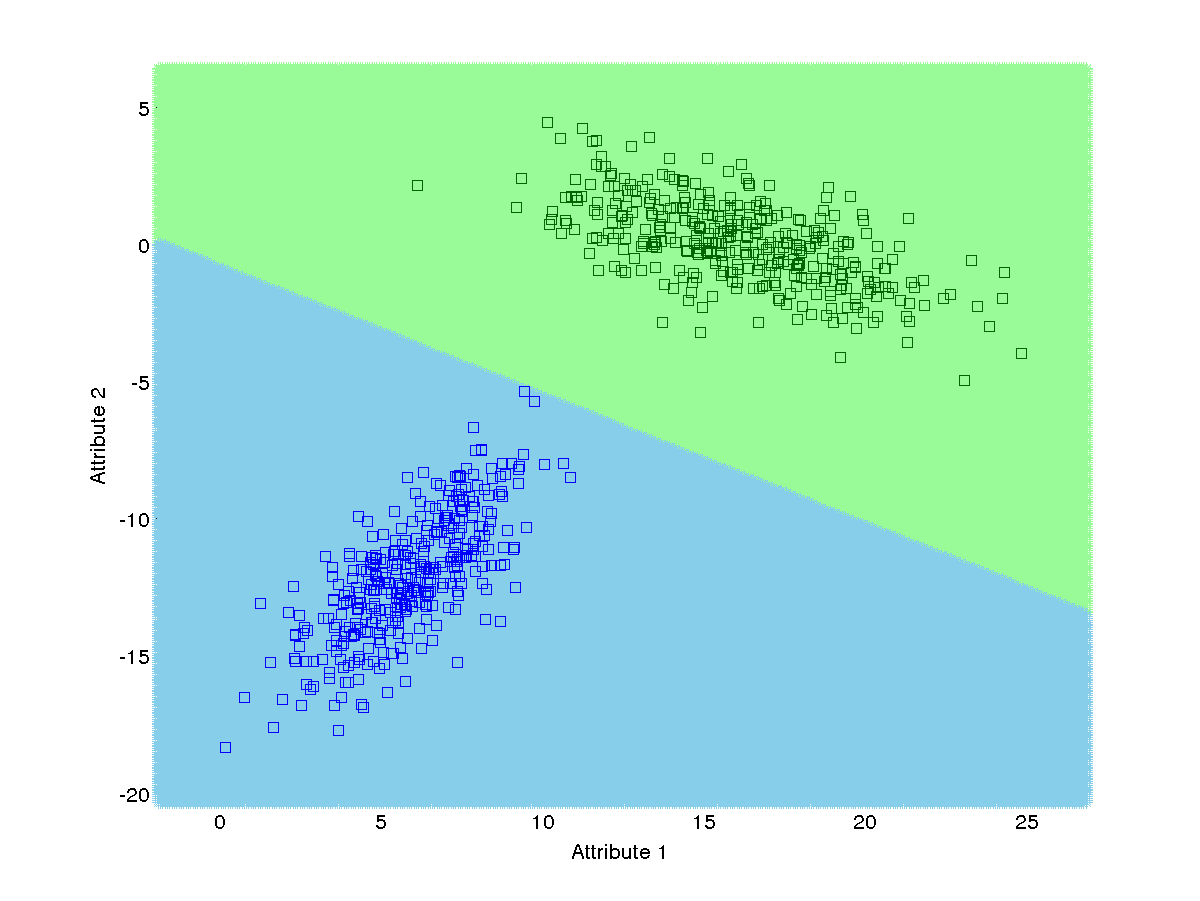
\includegraphics[width=40mm,height=30mm]{bayes/ls/pair/12/all_cov.png}&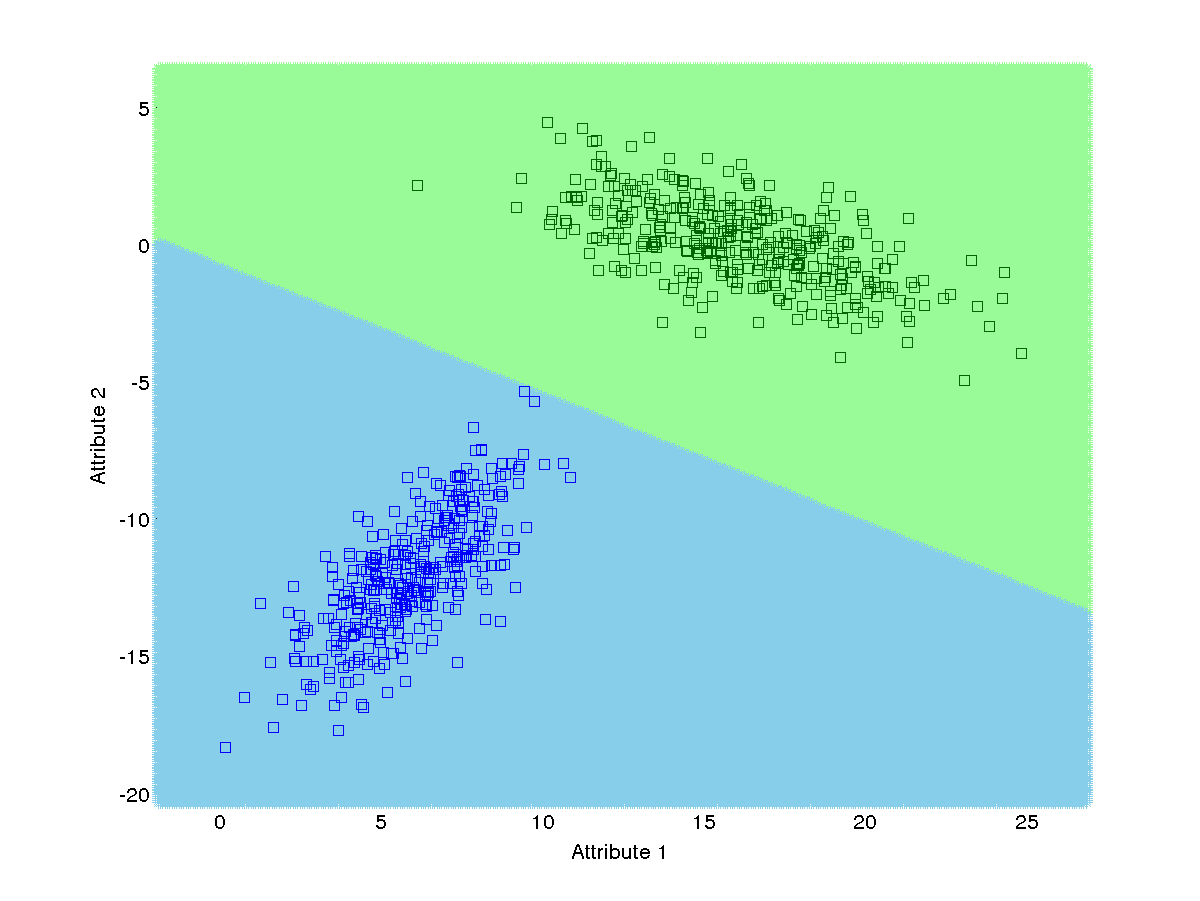
\includegraphics[width=40mm,height=30mm]{bayes/ls/pair/12/avg_cov.png}
					&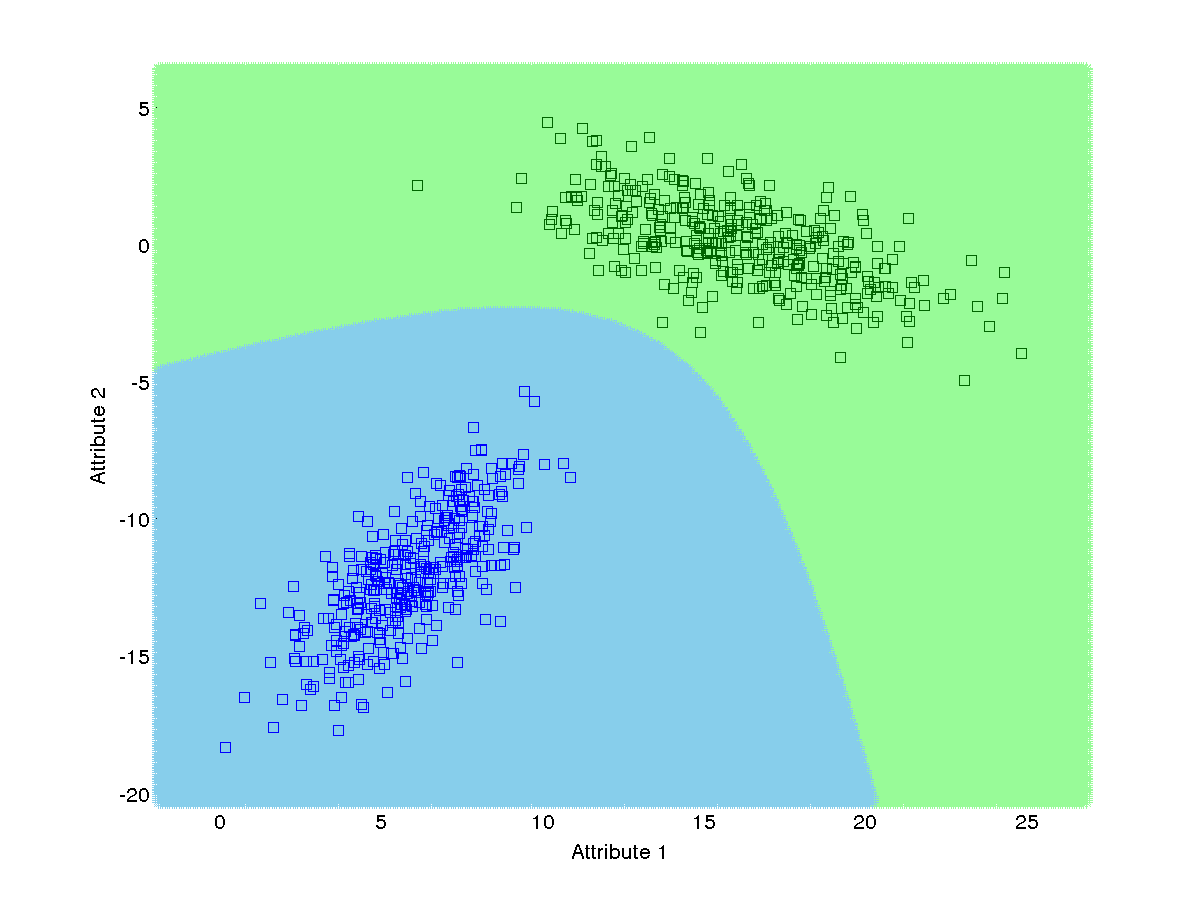
\includegraphics[width=40mm,height=30mm]{bayes/ls/pair/12/diff_cov.png}\\
					\hline
					1 and
					3&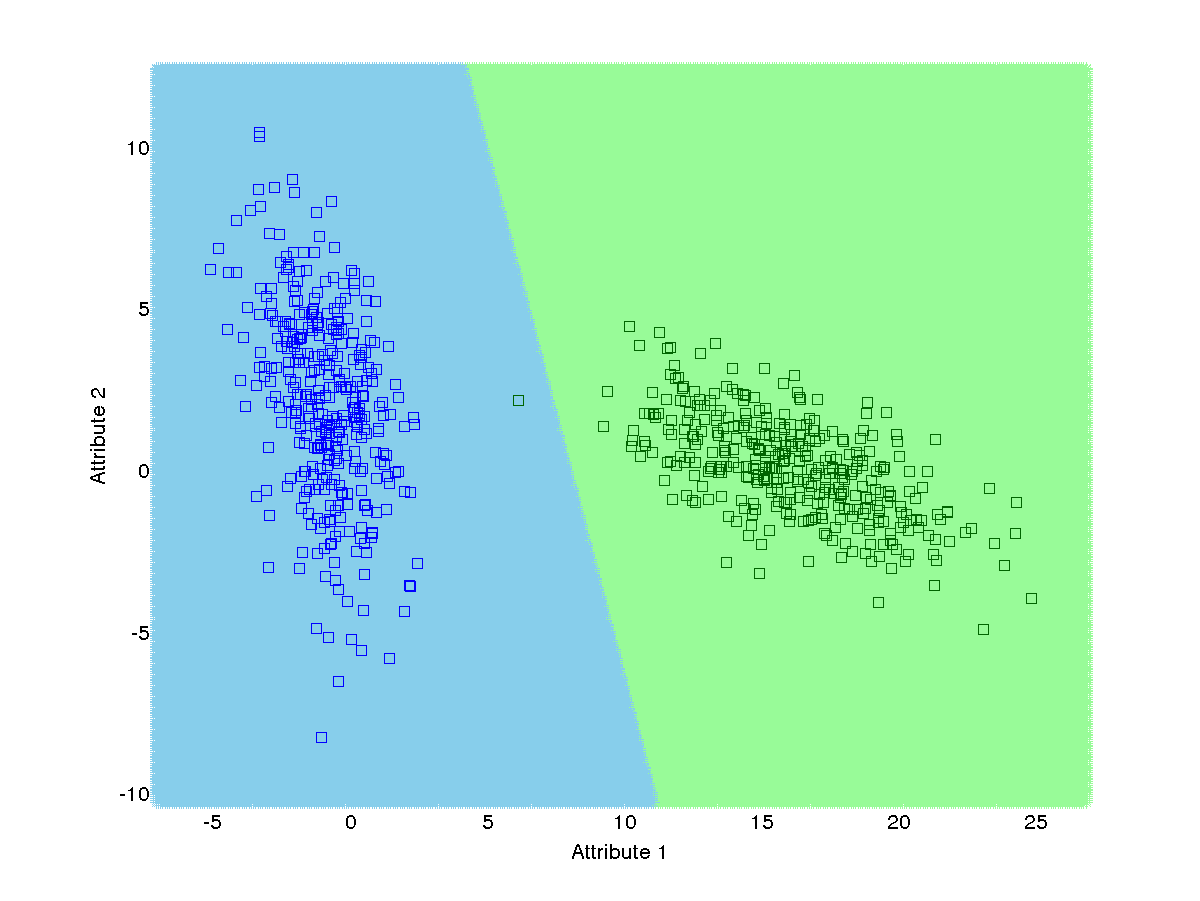
\includegraphics[width=40mm,height=30mm]{bayes/ls/pair/13/all_cov.png}&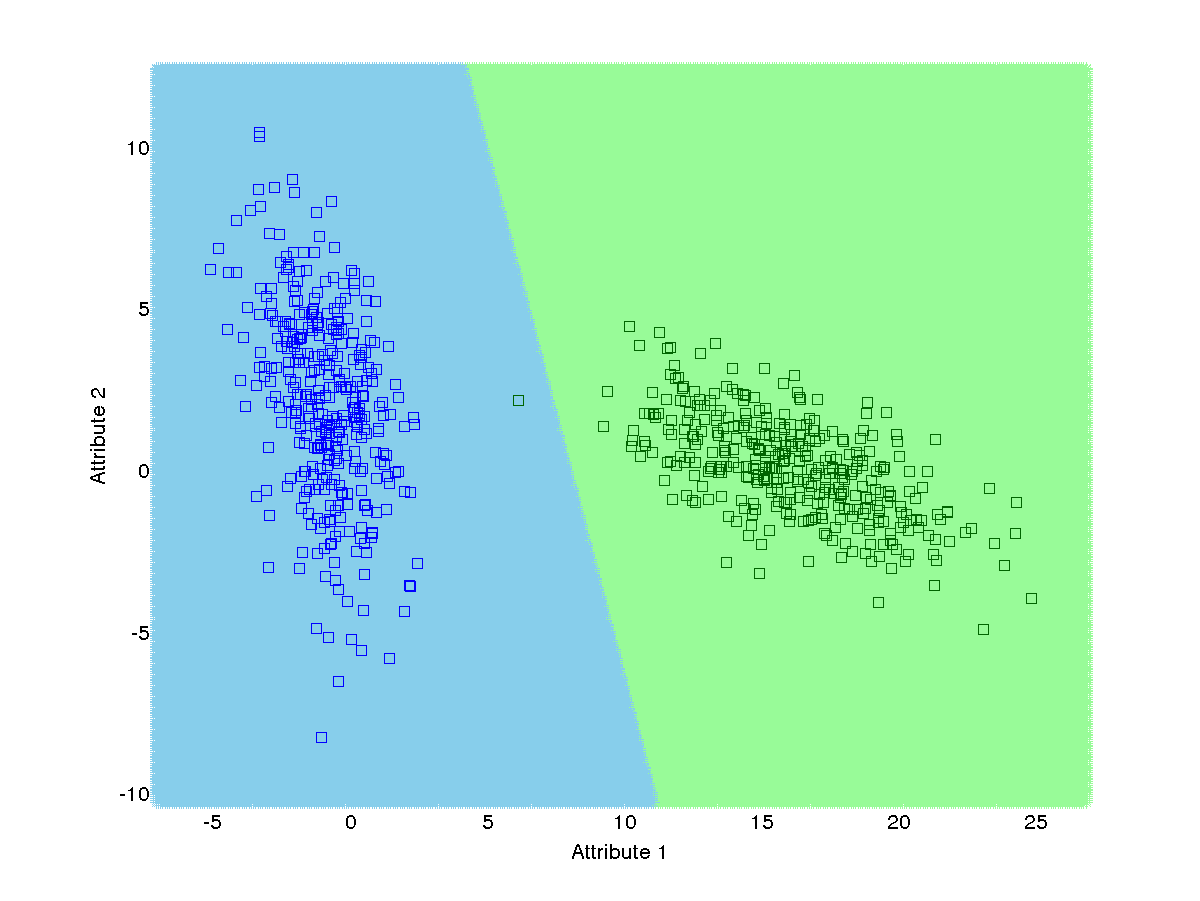
\includegraphics[width=40mm,height=30mm]{bayes/ls/pair/13/all_cov.png}
					&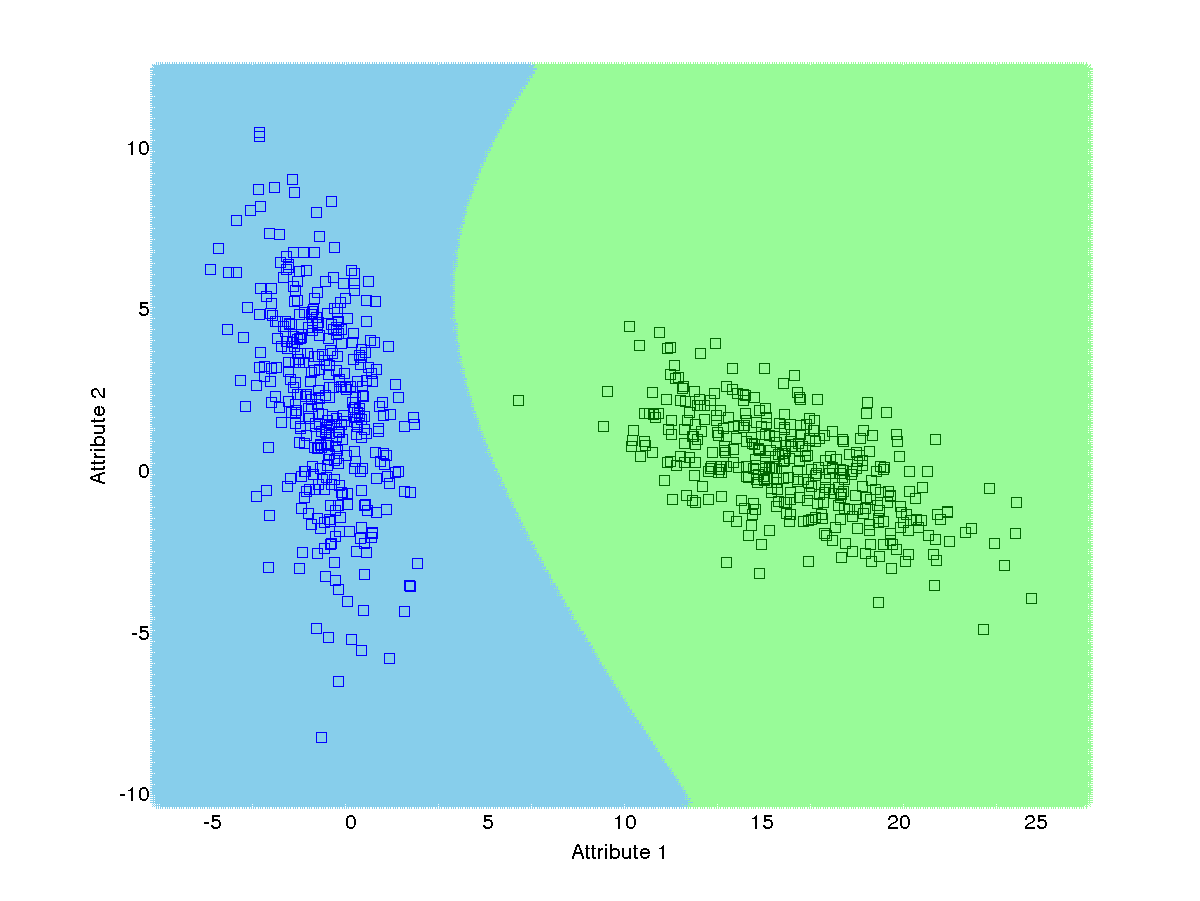
\includegraphics[width=40mm,height=30mm]{bayes/ls/pair/13/diff_cov.png}\\
					\hline
					2 and
					3&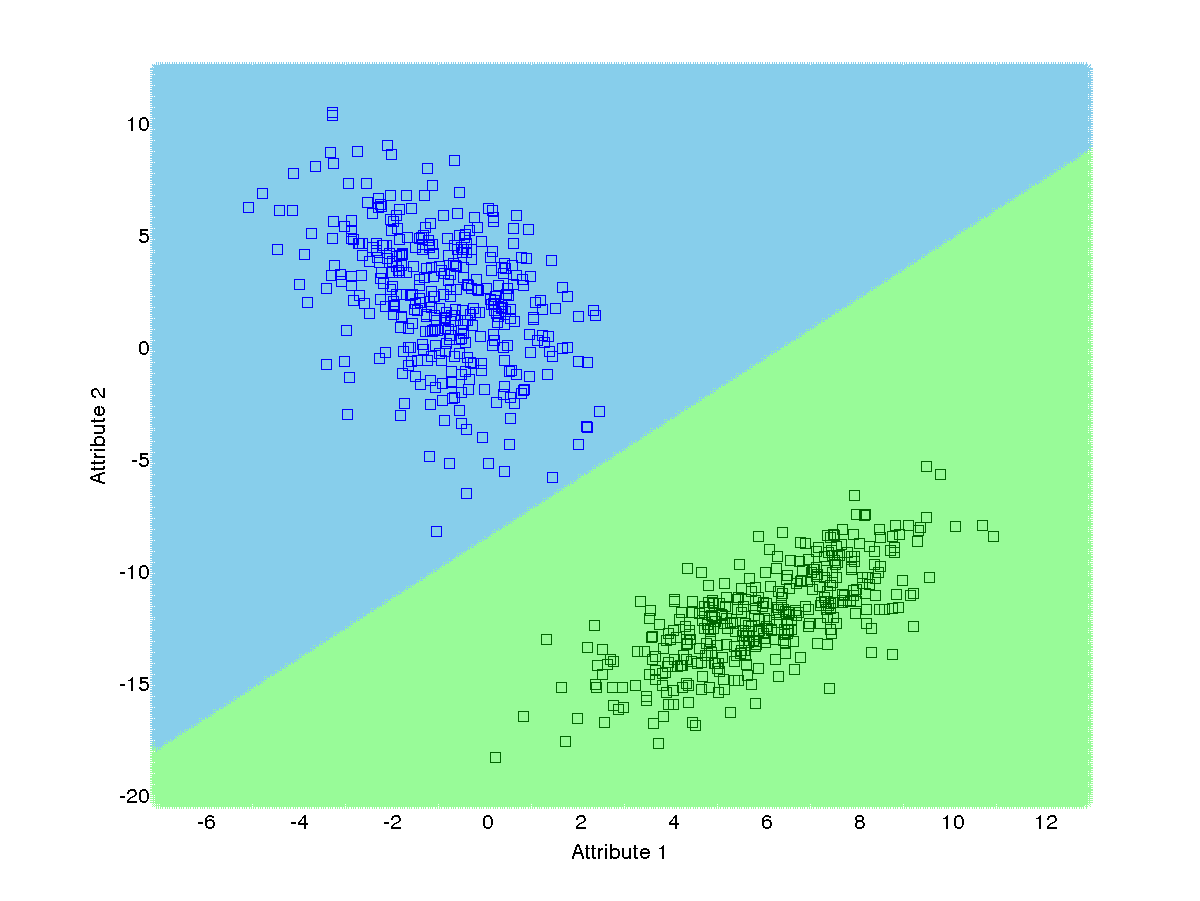
\includegraphics[width=40mm,height=30mm]{bayes/ls/pair/23/all_cov.png}&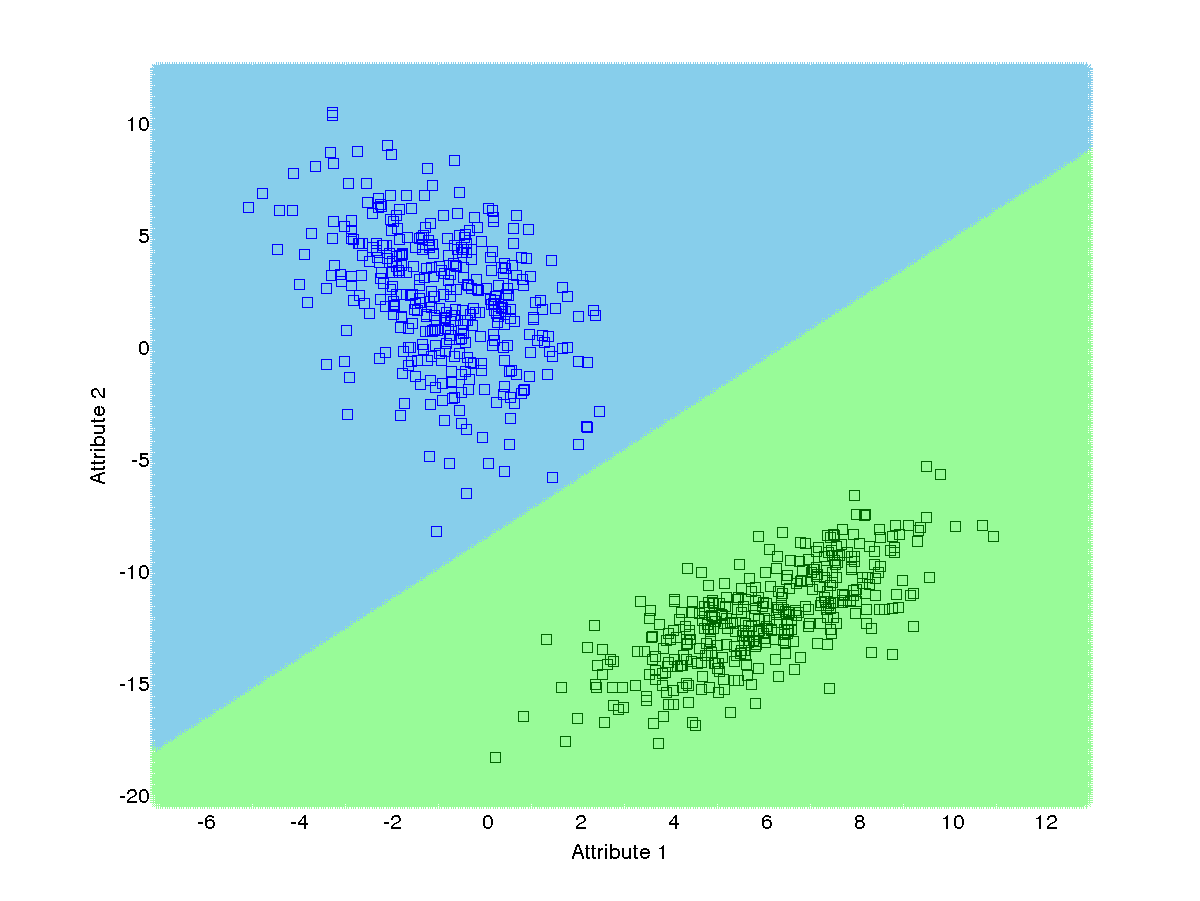
\includegraphics[width=40mm,height=30mm]{bayes/ls/pair/23/avg_cov.png}
					&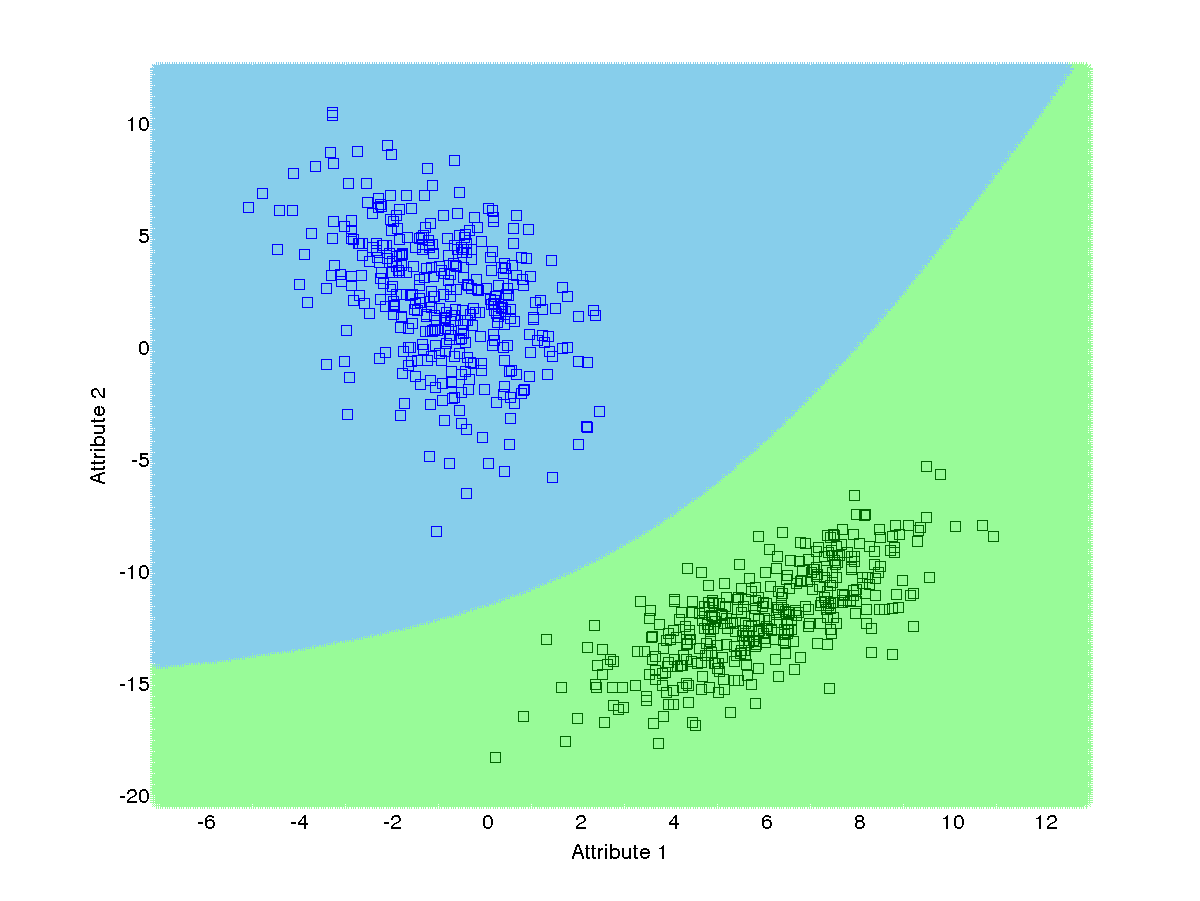
\includegraphics[width=40mm,height=30mm]{bayes/ls/pair/23/diff_cov.png}\\
					\hline
				\end{tabular}
				\caption{Decision region plot for every pair of classes}
			\end{figure}
		
			
		
		\begin{minipage}[t]{0.6\linewidth}
			\vspace{0pt} % [3]
			 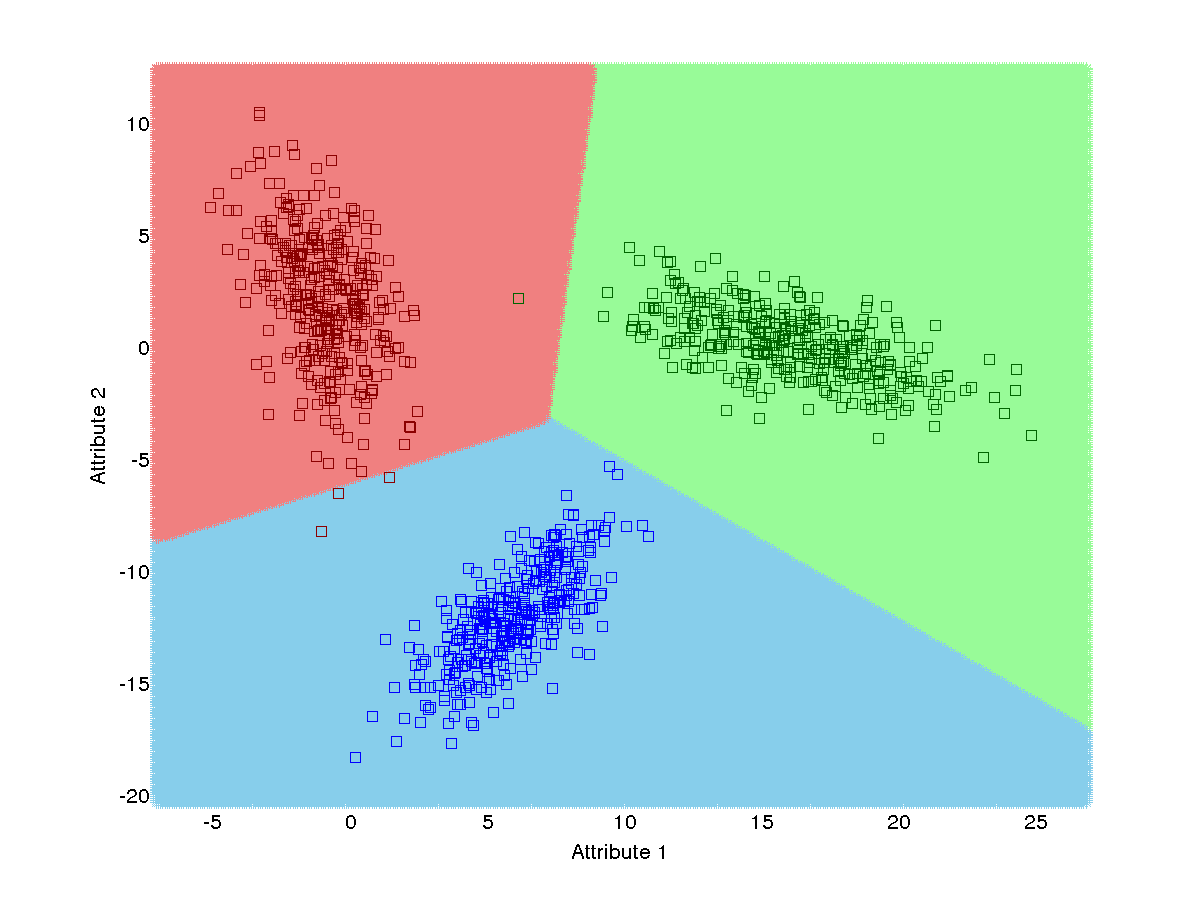
\includegraphics[width=\textwidth]{bayes/ls/all/all_cov.png}
		  	\captionof{figure}{ Decision region plot for all the classes together with the training data
superposed with alltogether covariance} % [4]
		  \label{gfx/image}	
		\end{minipage}
		\begin{minipage}[t]{0.2\linewidth} % [2]
		\vspace{10pt} % [3]
			Correct   : 374	\\
			Incorrect : 1	\\
			Acurracy  : 99.733 \\
		\begin{center}
			\begin{tabular}{ |c|c|c|c|c| }
			\hline
			& & \multicolumn{3}{| c |}{Predicted} \\
			\hline
			& & Class 1 & Class 2 & Class 3\\
			\hline
			\multirow{3}{*}{\rotatebox[origin=c]{90}{Act.}} & Class 1 & 125 & 0 & 0\\
			& Class 2 & 0 & 125 & 0\\
			& Class 3 & 0 & 1 & 124\\
			\hline
			\end{tabular}
			\end{center}
		\end{minipage}
	
		\begin{minipage}[t]{0.6\linewidth}
			\vspace{0pt} % [3]
			  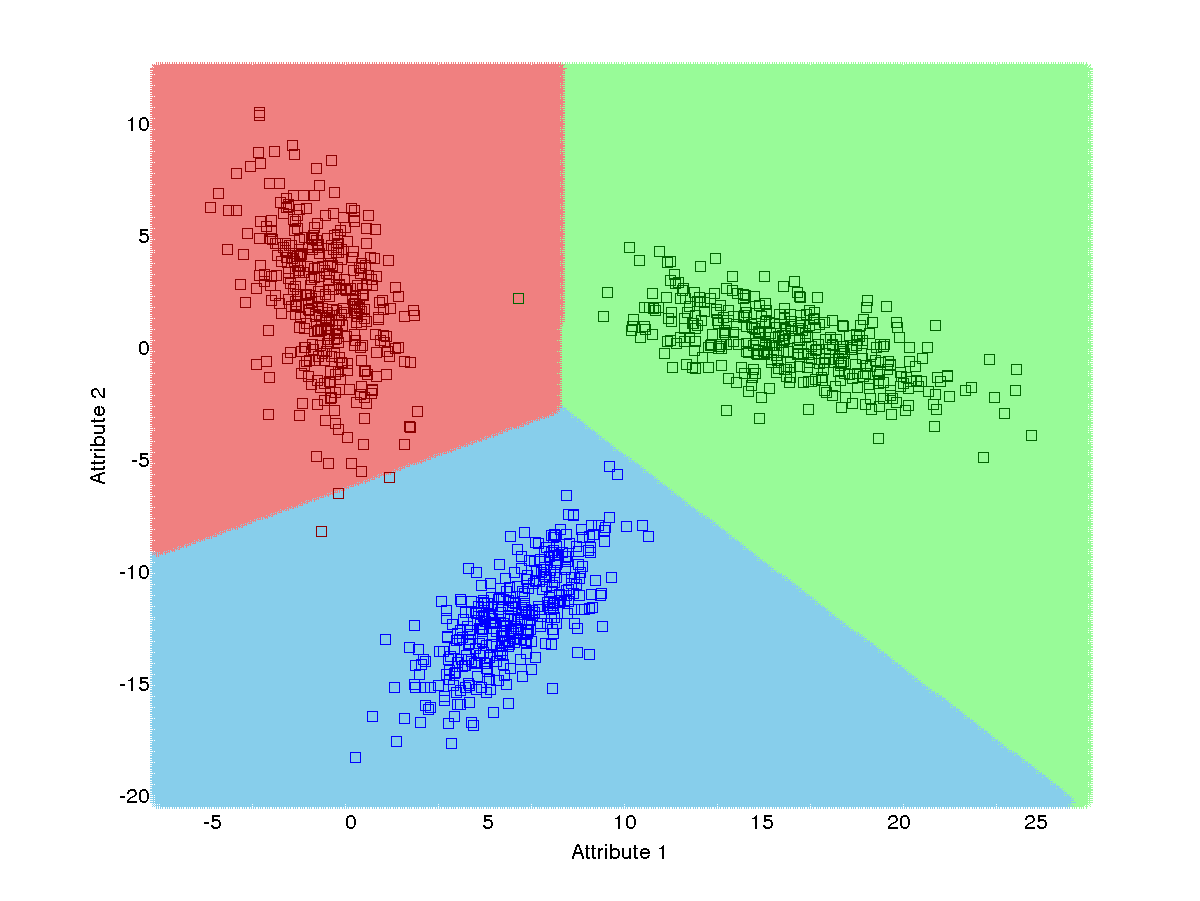
\includegraphics[width=\textwidth]{bayes/ls/all/avg_cov.png}
			  \captionof{figure}{ Decision region plot for all the classes together with the training data
 superposed with average covariance} % [4]
			  \label{gfx/image}	
			\end{minipage}
			\begin{minipage}[t]{0.2\linewidth} % [2]
			\vspace{10pt} % [3]
				Correct   : 374	\\
				Incorrect : 1	\\
				Acurracy  : 99.733 \\
			\begin{center}
				\begin{tabular}{ |c|c|c|c|c| }
				\hline
				& & \multicolumn{3}{| c |}{Predicted} \\
				\hline
				& & Class 1 & Class 2 & Class 3\\
				\hline
				\multirow{3}{*}{\rotatebox[origin=c]{90}{Act.}} & Class 1 & 125 & 0 & 0\\
				& Class 2 & 0 & 125 & 0\\
				& Class 3 & 0 & 1 & 124\\
				\hline
				\end{tabular}
				\end{center}
			\end{minipage}
			
		\begin{minipage}[t]{0.6\linewidth}
			\vspace{0pt} % [3]
			  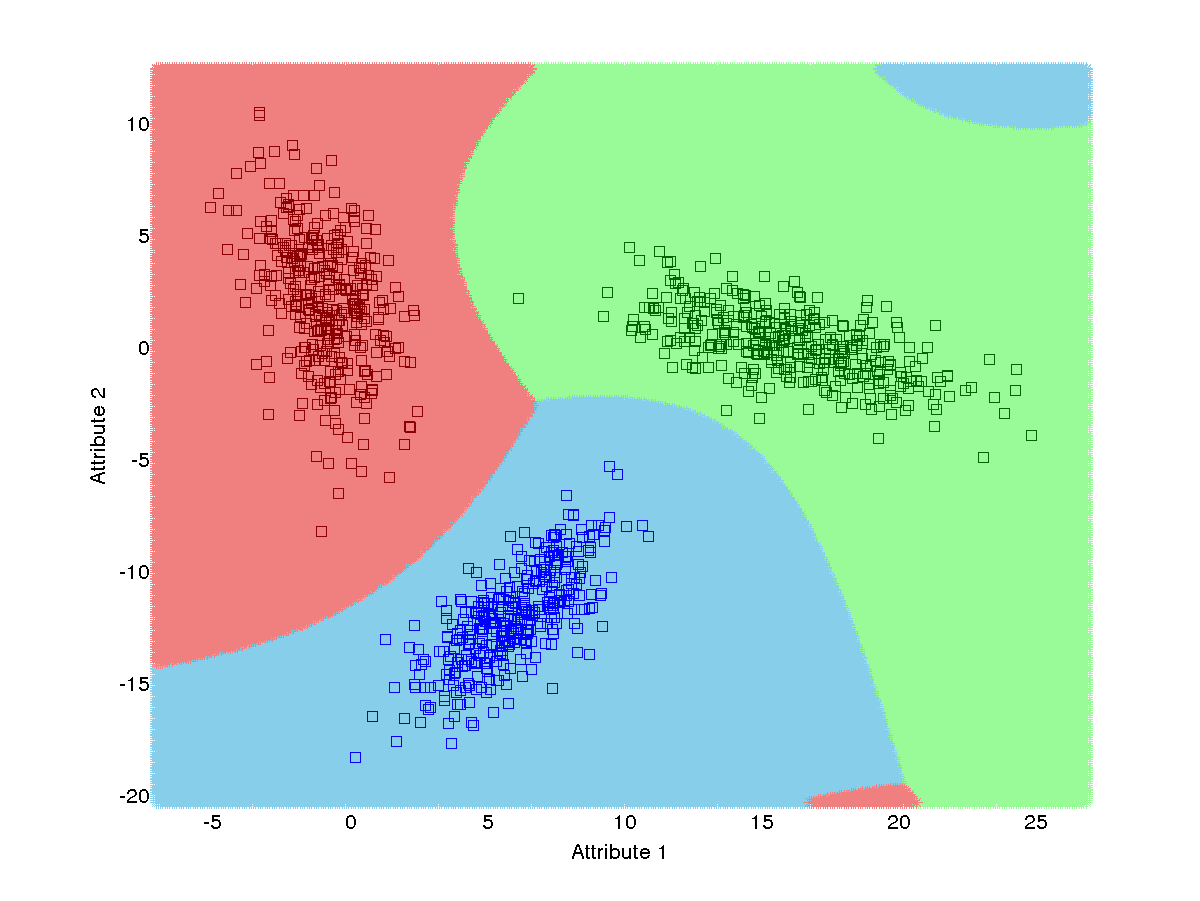
\includegraphics[width=\textwidth]{bayes/ls/all/diff_cov.png}
			  \captionof{figure}{ Decision region plot for all the classes together with the training data
 superposed with different covariance} % [4]
			  \label{gfx/image}	
			\end{minipage}
			\begin{minipage}[t]{0.2\linewidth} % [2]
			\vspace{10pt} % [3]
				Correct   : 375	\\
				Incorrect : 0	\\
				Acurracy  : 100 \\
			\begin{center}
				\begin{tabular}{ |c|c|c|c|c| }
				\hline
				& & \multicolumn{3}{| c |}{Predicted} \\
				\hline
				& & Class 1 & Class 2 & Class 3\\
				\hline
				\multirow{3}{*}{\rotatebox[origin=c]{90}{Act.}} & Class 1 & 125 & 0 & 0\\
				& Class 2 & 0 & 125 & 0\\
				& Class 3 & 0 & 0 & 125\\
				\hline
				\end{tabular}
				\end{center}
			\end{minipage}
			
	
		%%%%%%%%%%%%%%%%%%%%%%%%%%%%%%%%%%%%%%%%%%%%%%%%%%%%%%%%%5
	
		\subsubsection{Non-Linearly separable data set }
			
			\paragraph{Data of Interlocking Classes}

			\noindent
			
				%%%%%%%%%%%%%%%%%%%%%%%%%%%%%%%%%%%%%%%%%%%%%%%%%%%%%%%%%5
				
			

			\begin{minipage}[t]{0.6\linewidth}
			\vspace{0pt} % [3]
			  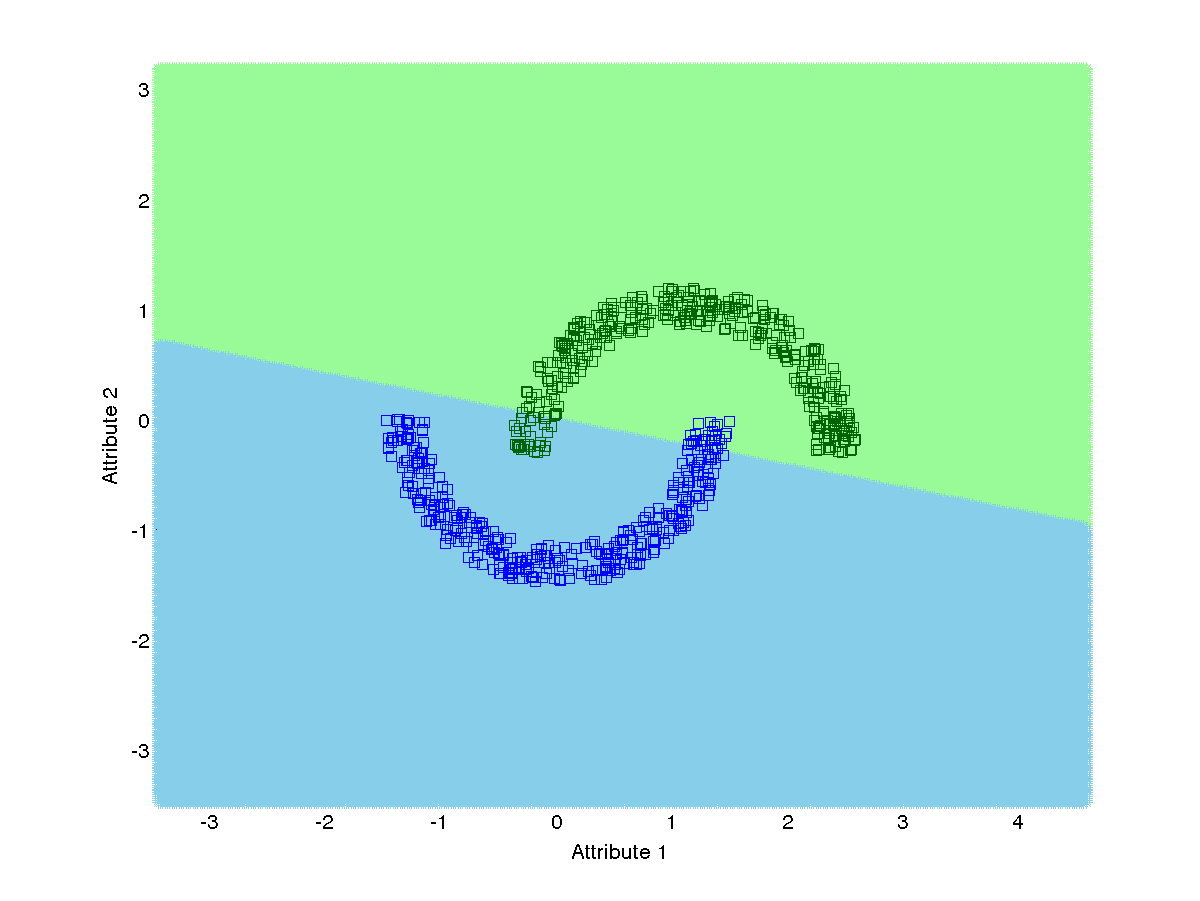
\includegraphics[width=\textwidth]{bayes/nls/interlock/all/all_cov.png}
			  \captionof{figure}{ Decision region plot for all the classes together with the training data
 superposed with alltogether covariance} % [4]
			  \label{gfx/image}	
			\end{minipage}
			\begin{minipage}[t]{0.2\linewidth} % [2]
			\vspace{10pt} % [3]
				Correct   : 239	\\
				Incorrect : 11	\\
				Acurracy  : 95.6000 \\
			\begin{center}
				\begin{tabular}{ |c|c|c|c| }
				\hline
				& & \multicolumn{2}{| c |}{Predicted} \\
				\hline
				& & Class 1 & Class 2\\
				\hline
				\multirow{3}{*}{\rotatebox[origin=c]{90}{Act.}} & Class 1 & 118 & 7 \\
				& Class 2 & 4 & 121\\
				\hline
				\end{tabular}
				\end{center}
			\end{minipage}
	
		\begin{minipage}[t]{0.6\linewidth}
			\vspace{0pt} % [3]
			  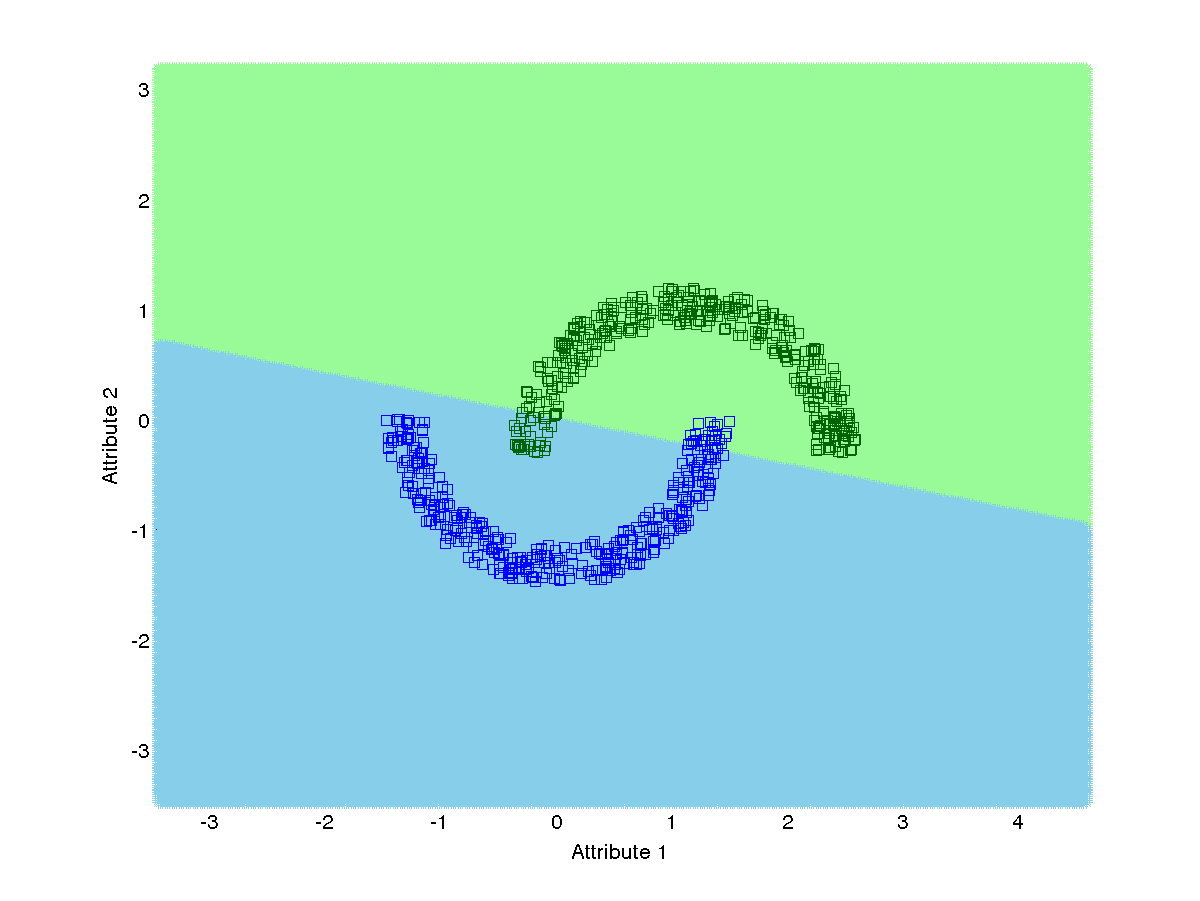
\includegraphics[width=\textwidth]{bayes/nls/interlock/all/avg_cov.png}
			  \captionof{figure}{ Decision region plot for all the classes together with the training data
 superposed with average covariance} % [4]
			  \label{gfx/image}	
			\end{minipage}
			\begin{minipage}[t]{0.2\linewidth} % [2]
			\vspace{10pt} % [3]
				Correct   : 239	\\
				Incorrect : 11	\\
				Acurracy  : 95.6000 \\
			\begin{center}
				\begin{tabular}{ |c|c|c|c| }
				\hline
				& & \multicolumn{2}{| c |}{Predicted} \\
				\hline
				& & Class 1 & Class 2\\
				\hline
				\multirow{3}{*}{\rotatebox[origin=c]{90}{Act.}} & Class 1 & 118 & 7 \\
				& Class 2 & 4 & 121\\
				\hline
				\end{tabular}
				\end{center}
			\end{minipage}
			
		\begin{minipage}[t]{0.6\linewidth}
			\vspace{0pt} % [3]
			  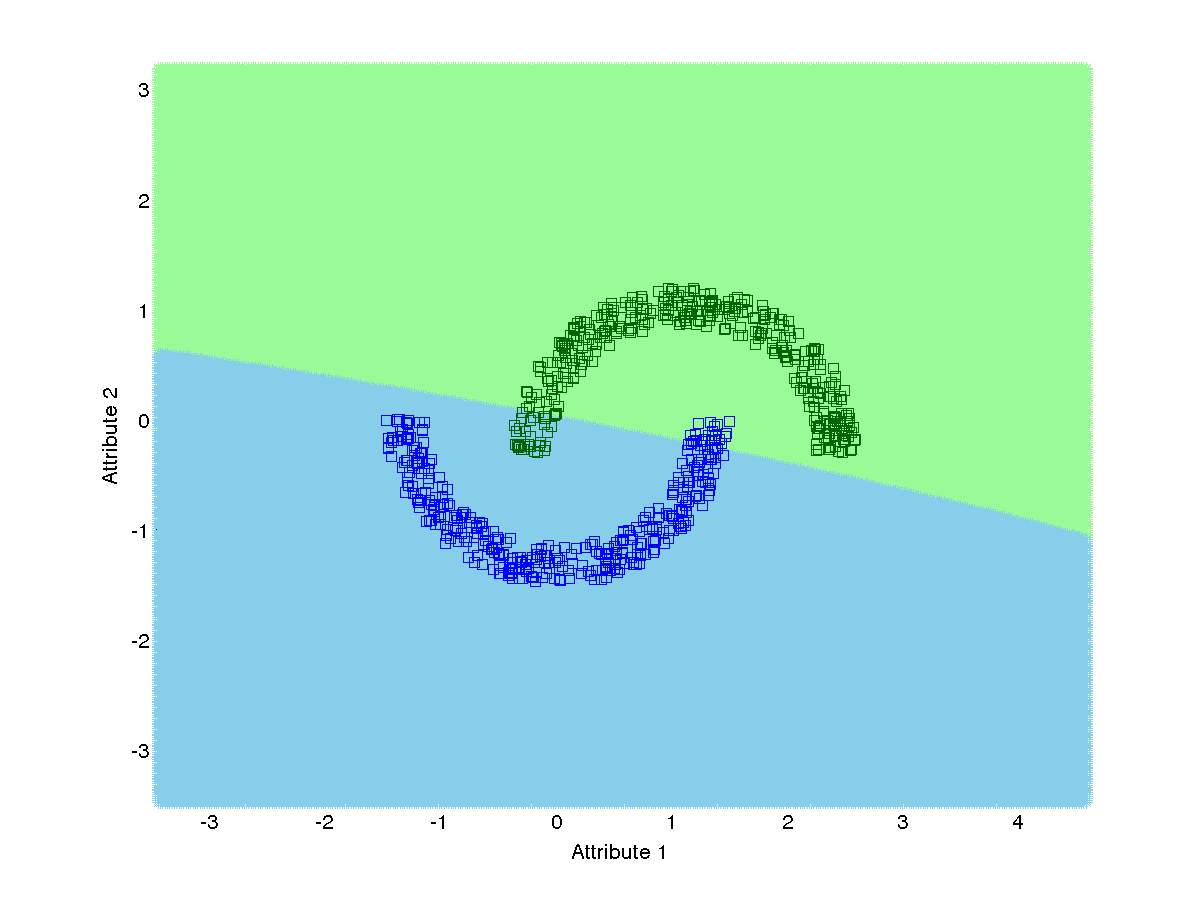
\includegraphics[width=\textwidth]{bayes/nls/interlock/all/diff_cov.png}
			  \captionof{figure}{ Decision region plot for all the classes together with the training data
 superposed with different covariance} % [4]
			  \label{gfx/image}	
			\end{minipage}
			\begin{minipage}[t]{0.2\linewidth} % [2]
			\vspace{10pt} % [3]
				Correct   : 240	\\
				Incorrect : 10	\\
				Acurracy  : 96 \\
			\begin{center}
				\begin{tabular}{ |c|c|c|c| }
				\hline
				& & \multicolumn{2}{| c |}{Predicted} \\
				\hline
				& & Class 1 & Class 2\\
				\hline
				\multirow{3}{*}{\rotatebox[origin=c]{90}{Act.}} & Class 1 & 118 & 7 \\
				& Class 2 & 3 & 122\\
				\hline
				\end{tabular}
				\end{center}
			\end{minipage}
			
				%%%%%%%%%%%%%%%%%%%%%%%%%%%%%%%%%%%%%%%%%%%%%%%%%%%%%%%%%5

  					
			\paragraph{A ring with a central mass} 

			\noindent
				
				%%%%%%%%%%%%%%%%%%%%%%%%%%%%%%%%%%%%%%%%%%%%%%%%%%%%%%%%%5
				
		
			\begin{minipage}[t]{0.6\linewidth}
			\vspace{0pt} % [3]
			  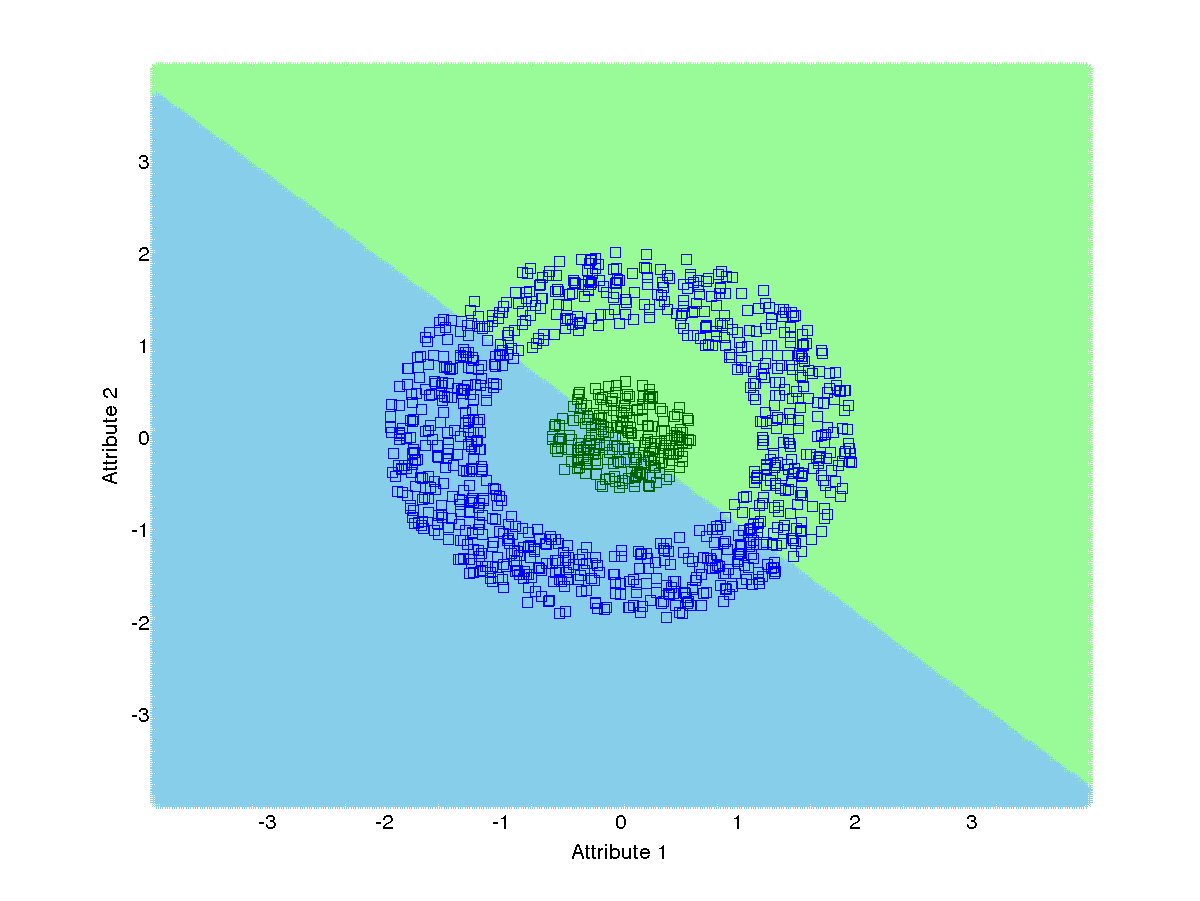
\includegraphics[width=\textwidth]{bayes/nls/ring/all/all_cov.png}
			  \captionof{figure}{ Decision region plot for all the classes together with the training data
 superposed with alltogether covariance} % [4]
			  \label{gfx/image}	
			\end{minipage}
			\begin{minipage}[t]{0.2\linewidth} % [2]
			\vspace{10pt} % [3]
				Correct   : 188	\\
				Incorrect : 187	\\
				Acurracy  : 50.133 \\
			\begin{center}
				\begin{tabular}{ |c|c|c|c| }
				\hline
				& & \multicolumn{2}{| c |}{Predicted} \\
				\hline
				& & Class 1 & Class 2\\
				\hline
				\multirow{3}{*}{\rotatebox[origin=c]{90}{Act.}} & Class 1 & 46 & 29 \\
				& Class 2 & 158 & 142\\
				\hline
				\end{tabular}
				\end{center}
			\end{minipage}
	
		\begin{minipage}[t]{0.6\linewidth}
			\vspace{0pt} % [3]
			  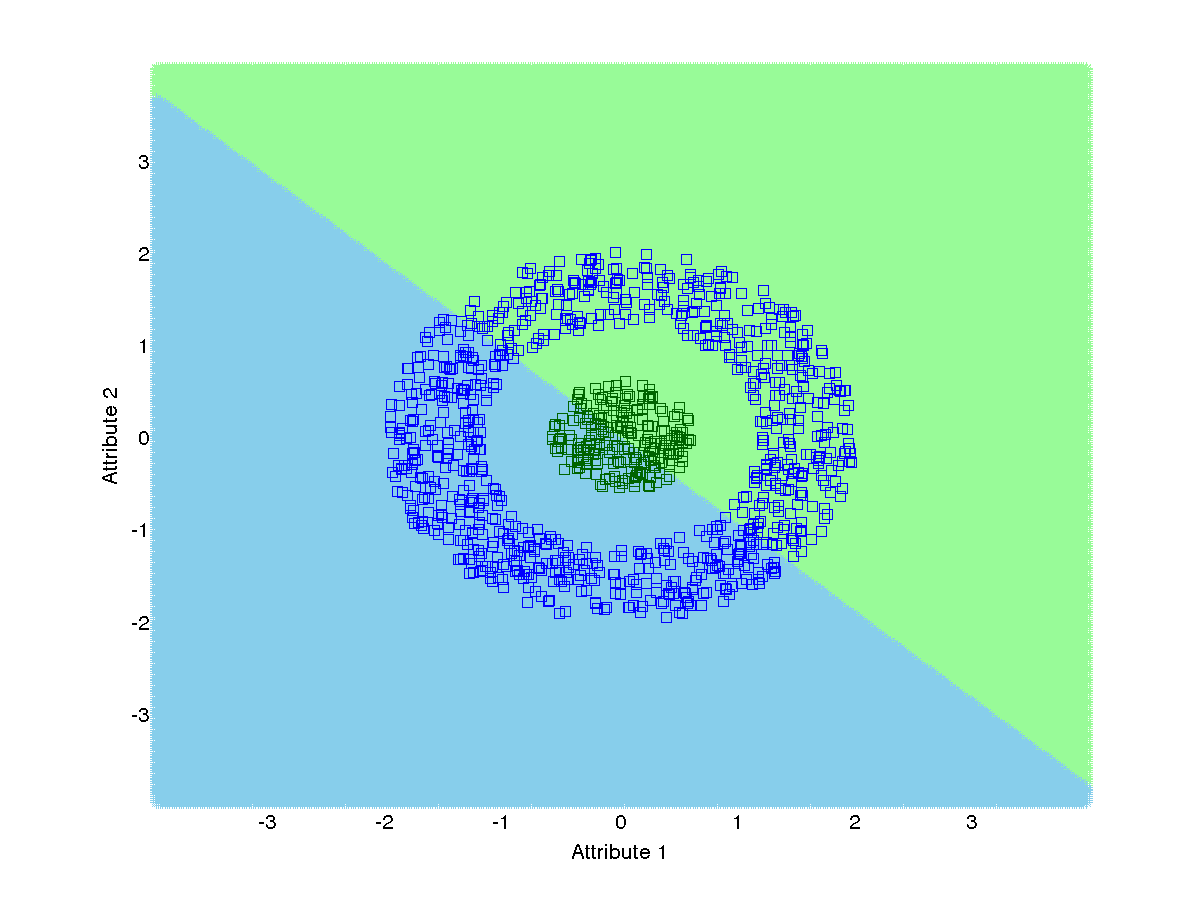
\includegraphics[width=\textwidth]{bayes/nls/ring/all/avg_cov.png}
			  \captionof{figure}{ Decision region plot for all the classes together with the training data
 superposed with average covariance} % [4]
			  \label{gfx/image}	
			\end{minipage}
			\begin{minipage}[t]{0.2\linewidth} % [2]
			\vspace{10pt} % [3]
				Correct   : 188	\\
				Incorrect : 187	\\
				Acurracy  : 50.133 \\
			\begin{center}
				\begin{tabular}{ |c|c|c|c| }
				\hline
				& & \multicolumn{2}{| c |}{Predicted} \\
				\hline
				& & Class 1 & Class 2\\
				\hline
				\multirow{3}{*}{\rotatebox[origin=c]{90}{Act.}} & Class 1 & 46 & 29 \\
				& Class 2 & 158 & 142\\
				\hline
				\end{tabular}
				\end{center}
			\end{minipage}
			
		\begin{minipage}[t]{0.6\linewidth}
			\vspace{0pt} % [3]
			  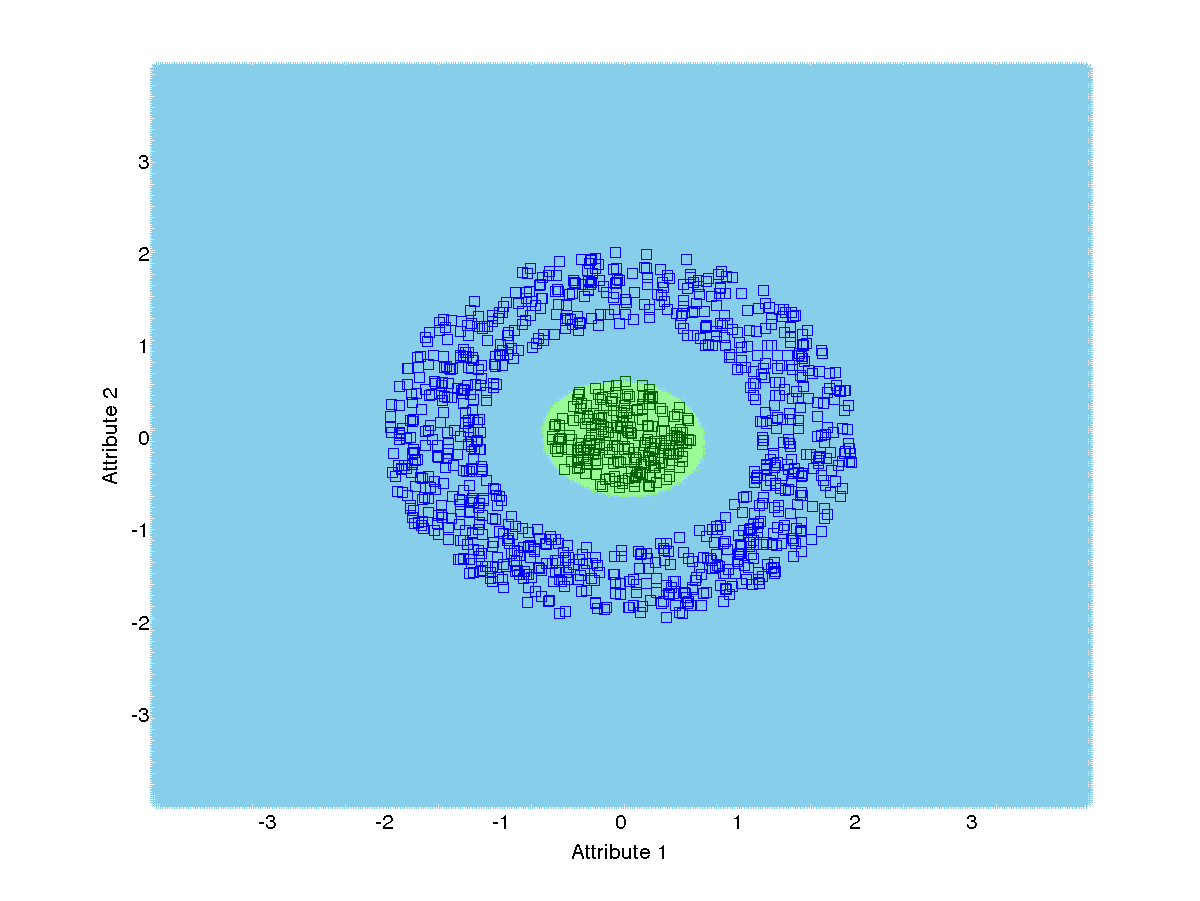
\includegraphics[width=\textwidth]{bayes/nls/ring/all/diff_cov.png}
			  \captionof{figure}{ Decision region plot for all the classes together with the training data
 superposed with different covariance} % [4]
			  \label{gfx/image}	
			\end{minipage}
			\begin{minipage}[t]{0.2\linewidth} % [2]
			\vspace{10pt} % [3]
				Correct   : 375	\\
				Incorrect : 0	\\
				Acurracy  : 100 \\
			\begin{center}
				\begin{tabular}{ |c|c|c|c| }
				\hline
				& & \multicolumn{2}{| c |}{Predicted} \\
				\hline
				& & Class 1 & Class 2\\
				\hline
				\multirow{3}{*}{\rotatebox[origin=c]{90}{Act.}} & Class 1 & 75 & 0 \\
				& Class 2 & 0 & 300\\
				\hline
				\end{tabular}
				\end{center}
			\end{minipage}
				%%%%%%%%%%%%%%%%%%%%%%%%%%%%%%%%%%%%%%%%%%%%%%%%%%%%%%%%%5
			

			\paragraph{Spiral Dataset}

			\noindent

		%%%%%%%%%%%%%%%%%%%%%%%%%%%%%%%%%%%%%%%%%%%%%%%%%%%%%%%%%5
				
		
			\begin{minipage}[t]{0.6\linewidth}
			\vspace{0pt} % [3]
			  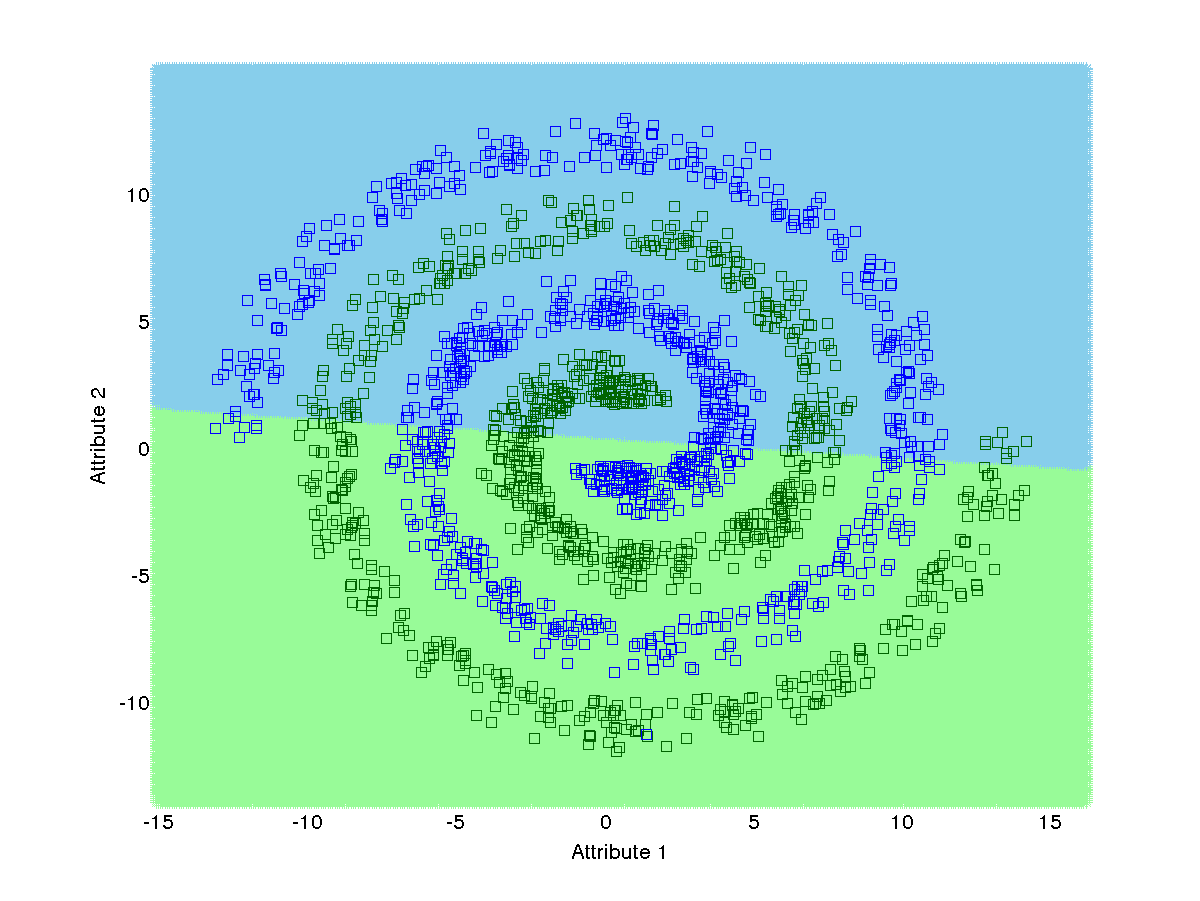
\includegraphics[width=\textwidth]{bayes/nls/spiral/all/all_cov.png}
			  \captionof{figure}{ Decision region plot for all the classes together with the training data
 superposed with alltogether covariance} % [4]
			  \label{gfx/image}	
			\end{minipage}
			\begin{minipage}[t]{0.2\linewidth} % [2]
			\vspace{10pt} % [3]
				Correct   : 188	\\
				Incorrect : 187	\\
				Acurracy  : 50.133 \\
			\begin{center}
				\begin{tabular}{ |c|c|c|c| }
				\hline
				& & \multicolumn{2}{| c |}{Predicted} \\
				\hline
				& & Class 1 & Class 2\\
				\hline
				\multirow{3}{*}{\rotatebox[origin=c]{90}{Act.}} & Class 1 & 46 & 29 \\
				& Class 2 & 158 & 142\\
				\hline
				\end{tabular}
				\end{center}
			\end{minipage}
	
		\begin{minipage}[t]{0.6\linewidth}
			\vspace{0pt} % [3]
			  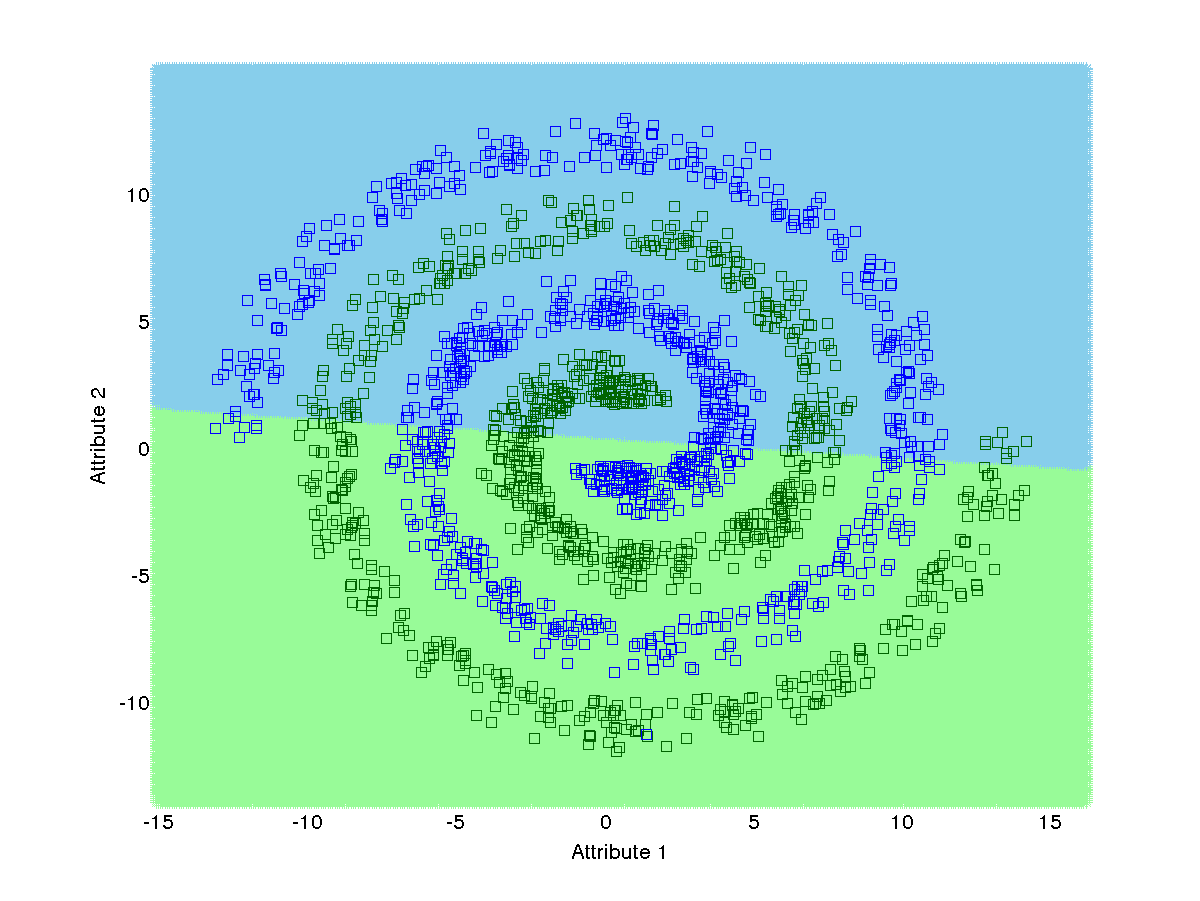
\includegraphics[width=\textwidth]{bayes/nls/spiral/all/avg_cov.png}
			  \captionof{figure}{ Decision region plot for all the classes together with the training data
 superposed with average covariance} % [4]
			  \label{gfx/image}	
			\end{minipage}
			\begin{minipage}[t]{0.2\linewidth} % [2]
			\vspace{10pt} % [3]
				Correct   : 188	\\
				Incorrect : 187	\\
				Acurracy  : 50.133 \\
			\begin{center}
				\begin{tabular}{ |c|c|c|c| }
				\hline
				& & \multicolumn{2}{| c |}{Predicted} \\
				\hline
				& & Class 1 & Class 2\\
				\hline
				\multirow{3}{*}{\rotatebox[origin=c]{90}{Act.}} & Class 1 & 46 & 29 \\
				& Class 2 & 158 & 142\\
				\hline
				\end{tabular}
				\end{center}
			\end{minipage}
			
		\begin{minipage}[t]{0.6\linewidth}
			\vspace{0pt} % [3]
			  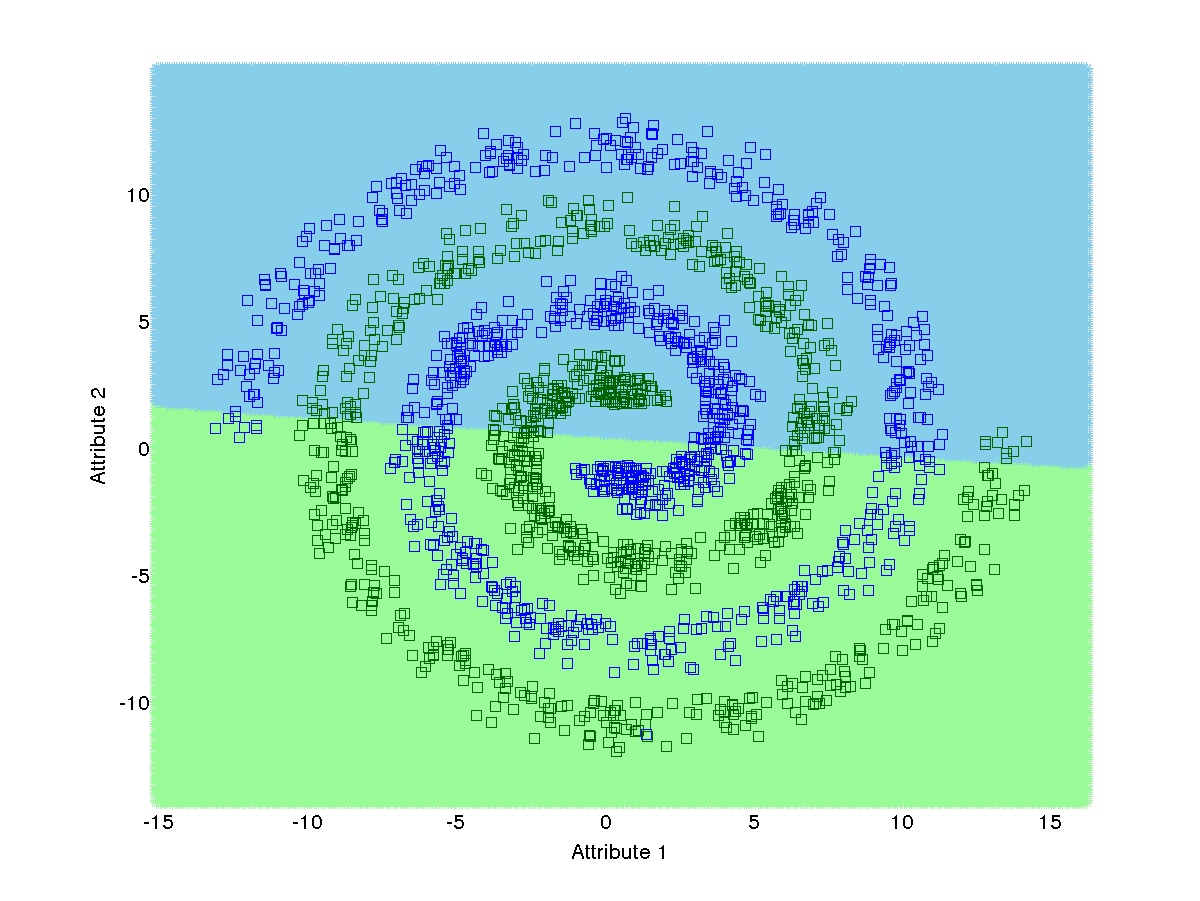
\includegraphics[width=\textwidth]{bayes/nls/spiral/all/diff_cov.png}
			  \captionof{figure}{ Decision region plot for all the classes together with the training data
 superposed with different covariance} % [4]
			  \label{gfx/image}	
			\end{minipage}
			\begin{minipage}[t]{0.2\linewidth} % [2]
			\vspace{10pt} % [3]
				Correct   : 375	\\
				Incorrect : 0	\\
				Acurracy  : 100 \\
			\begin{center}
				\begin{tabular}{ |c|c|c|c| }
				\hline
				& & \multicolumn{2}{| c |}{Predicted} \\
				\hline
				& & Class 1 & Class 2\\
				\hline
				\multirow{3}{*}{\rotatebox[origin=c]{90}{Act.}} & Class 1 & 75 & 0 \\
				& Class 2 & 0 & 300\\
				\hline
				\end{tabular}
				\end{center}
			\end{minipage}
				%%%%%%%%%%%%%%%%%%%%%%%%%%%%%%%%%%%%%%%%%%%%%%%%%%%%%%%%%5

			
		\subsubsection{Overlapping data set}
			%%%%%%%%%%%%%%%%%%%%%%%%%%%%%%%%%%%%%%%%%%%%%%%%%%%%%%%%%5
				
			\begin{figure}
			\begin{tabular}{|c|c|c|c|}
				\hline
				Pair/Cov &  Alltogther & Average & Different	\\
				\hline
				1 and
				2&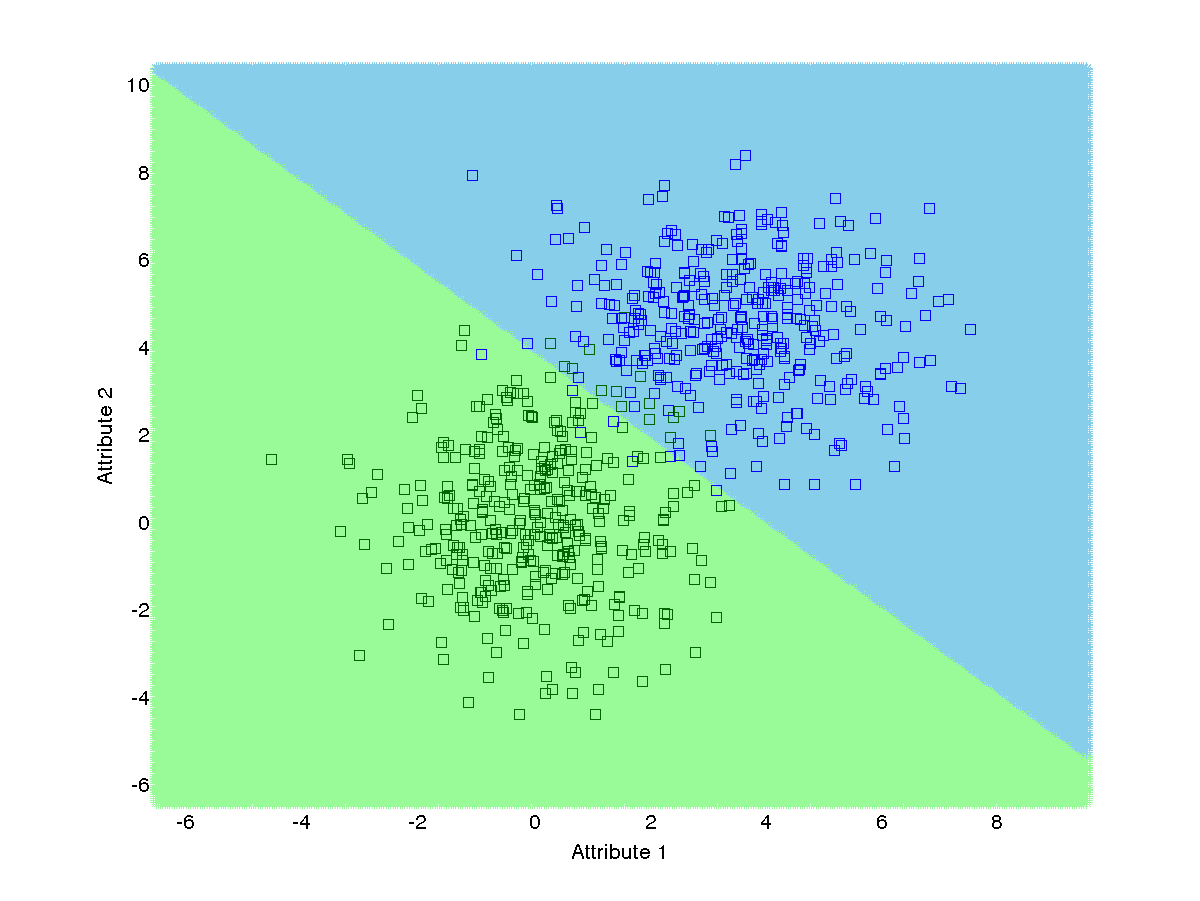
\includegraphics[width=40mm,height=30mm]{bayes/over/pair/12/all_cov.png}&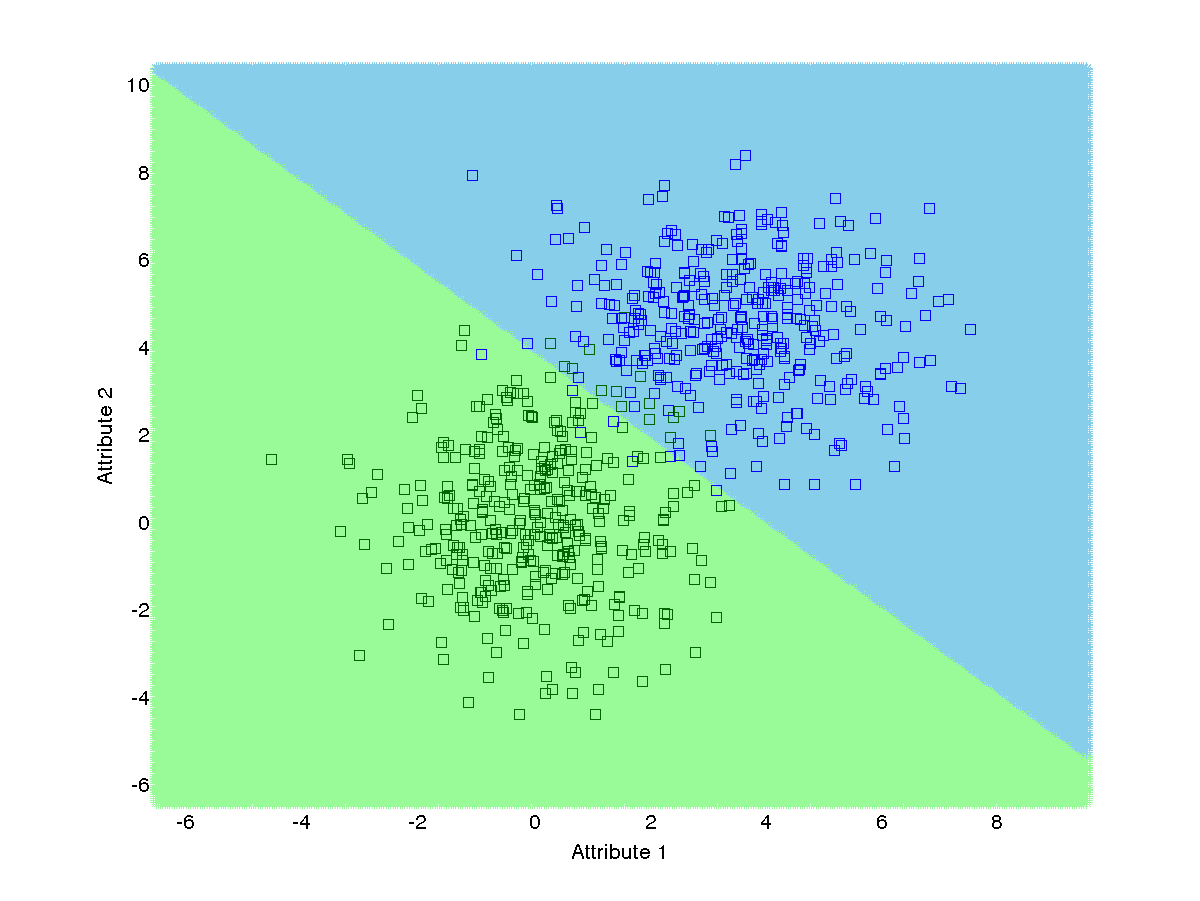
\includegraphics[width=40mm,height=30mm]{bayes/over/pair/12/avg_cov.png}
				&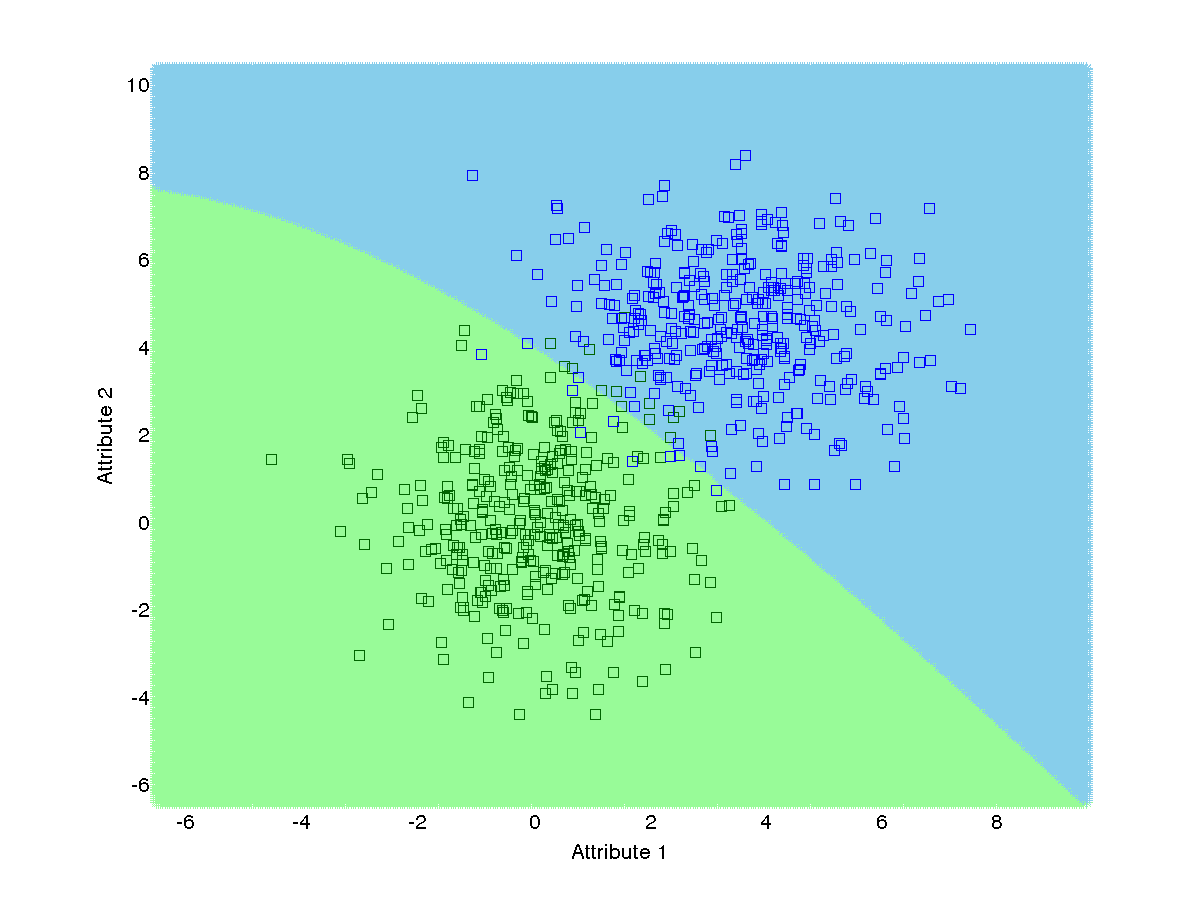
\includegraphics[width=40mm,height=30mm]{bayes/over/pair/12/diff_cov.png}\\
				\hline
				1 and
				3&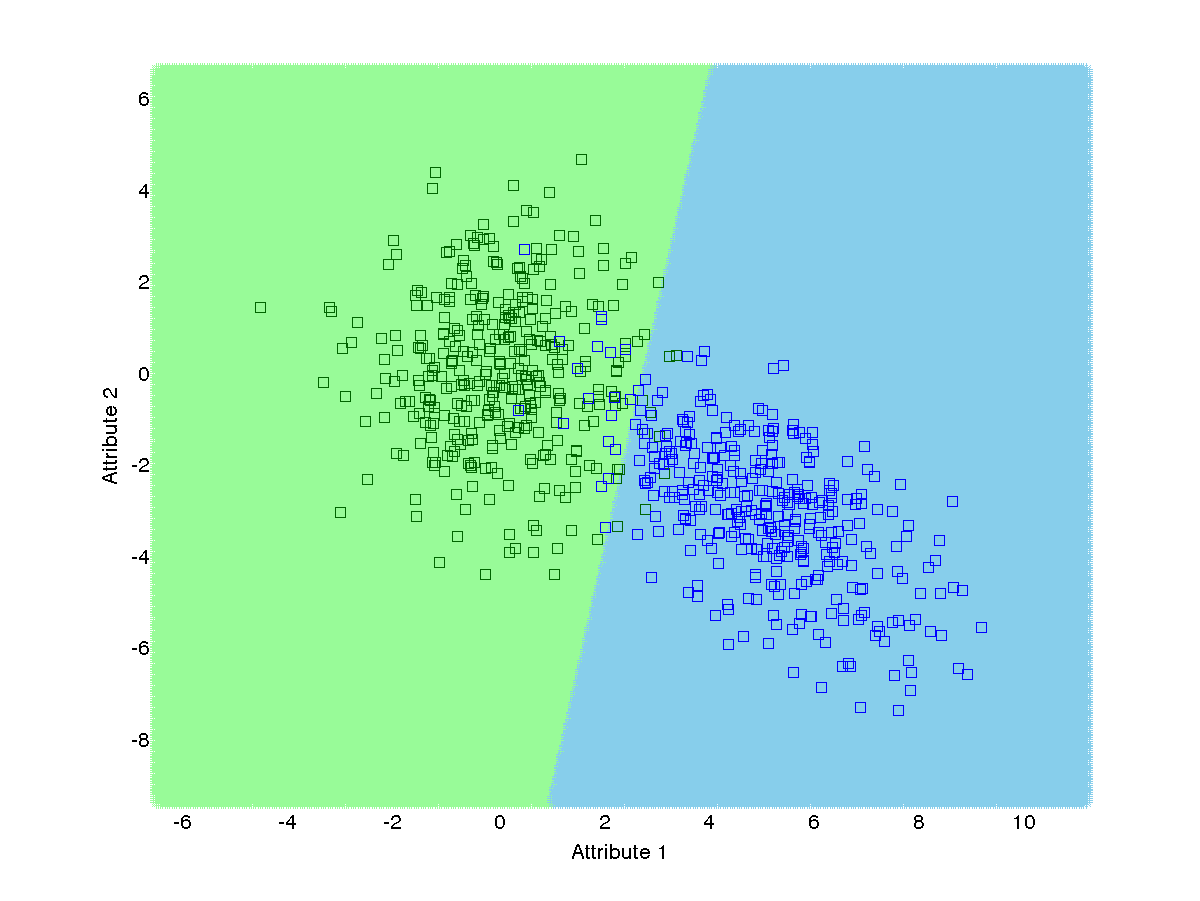
\includegraphics[width=40mm,height=30mm]{bayes/over/pair/13/all_cov.png}&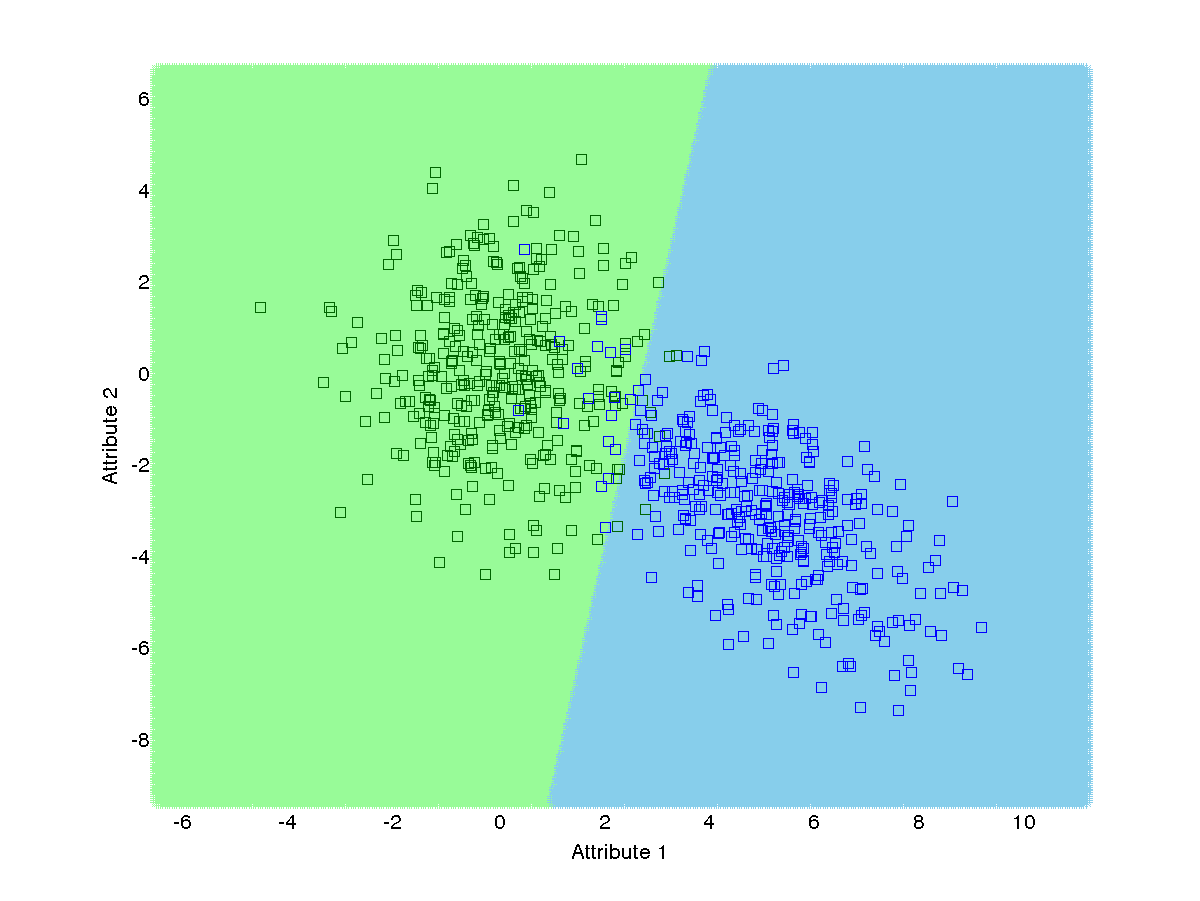
\includegraphics[width=40mm,height=30mm]{bayes/over/pair/13/avg_cov.png}
				&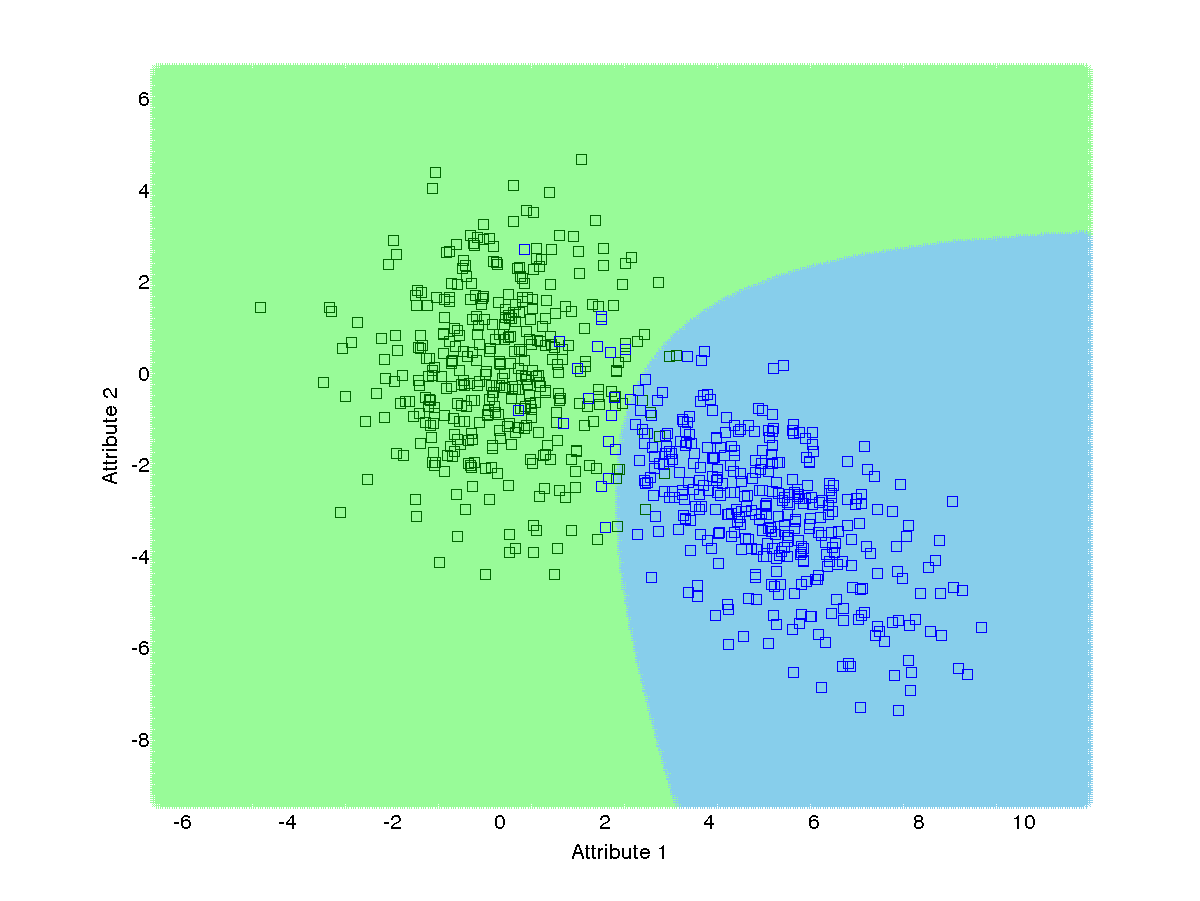
\includegraphics[width=40mm,height=30mm]{bayes/over/pair/13/diff_cov.png}\\
				\hline
				1 and
				4&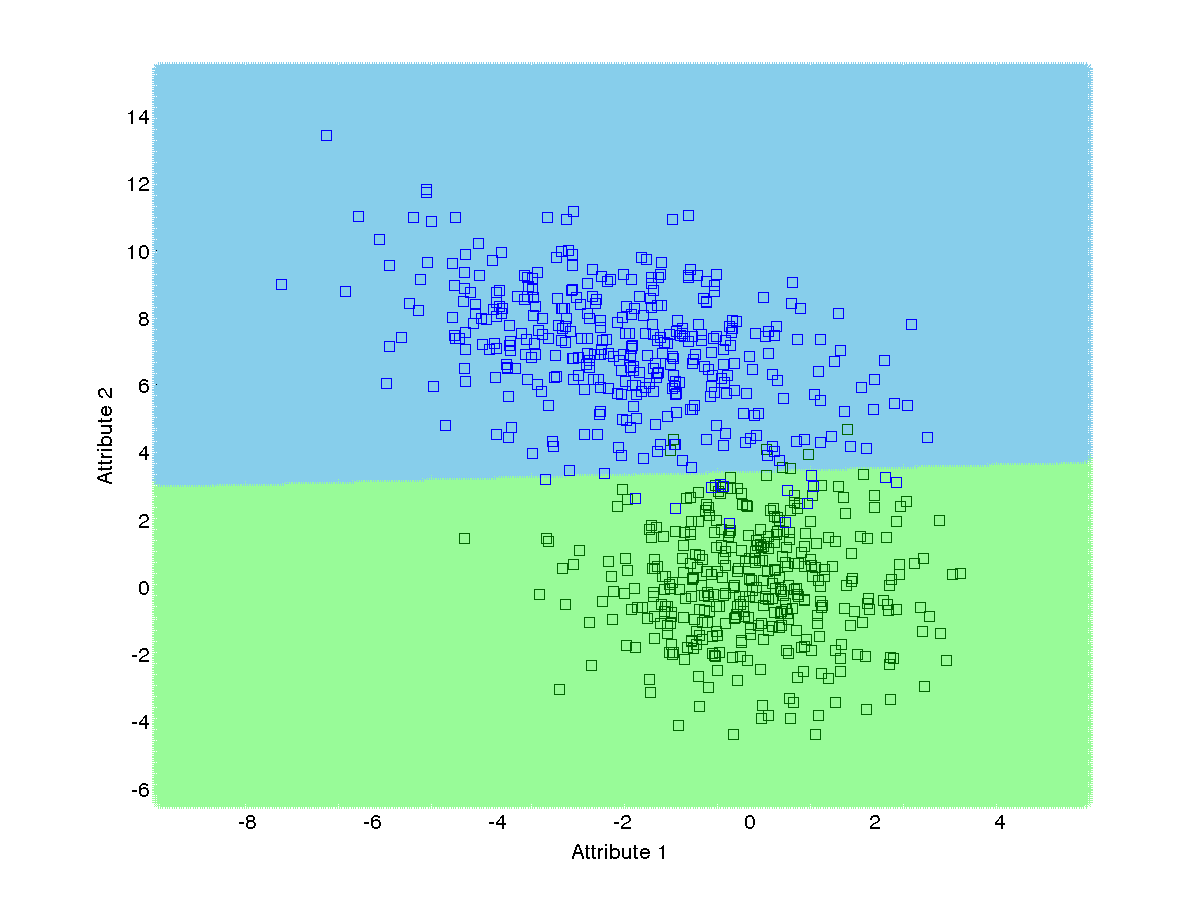
\includegraphics[width=40mm,height=30mm]{bayes/over/pair/14/all_cov.png}&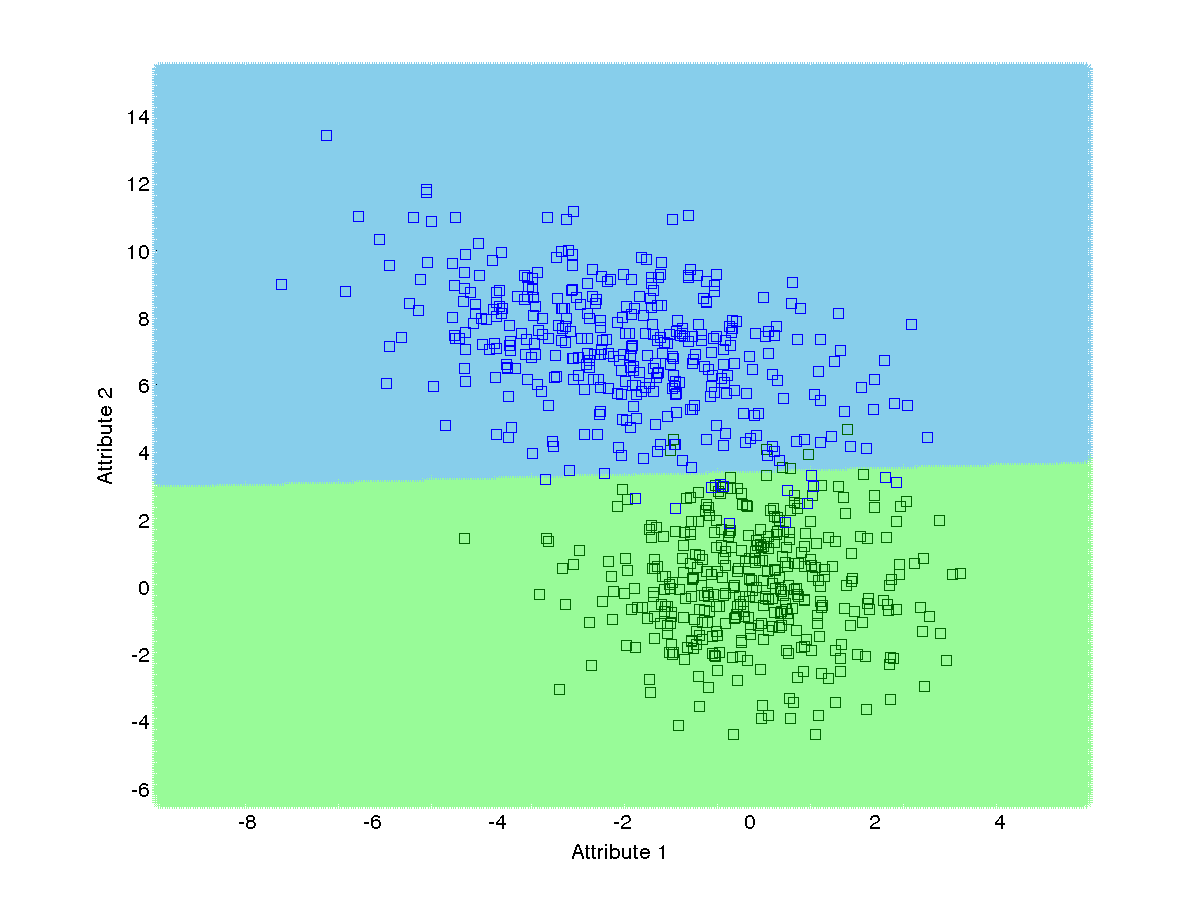
\includegraphics[width=40mm,height=30mm]{bayes/over/pair/14/avg_cov.png}
				&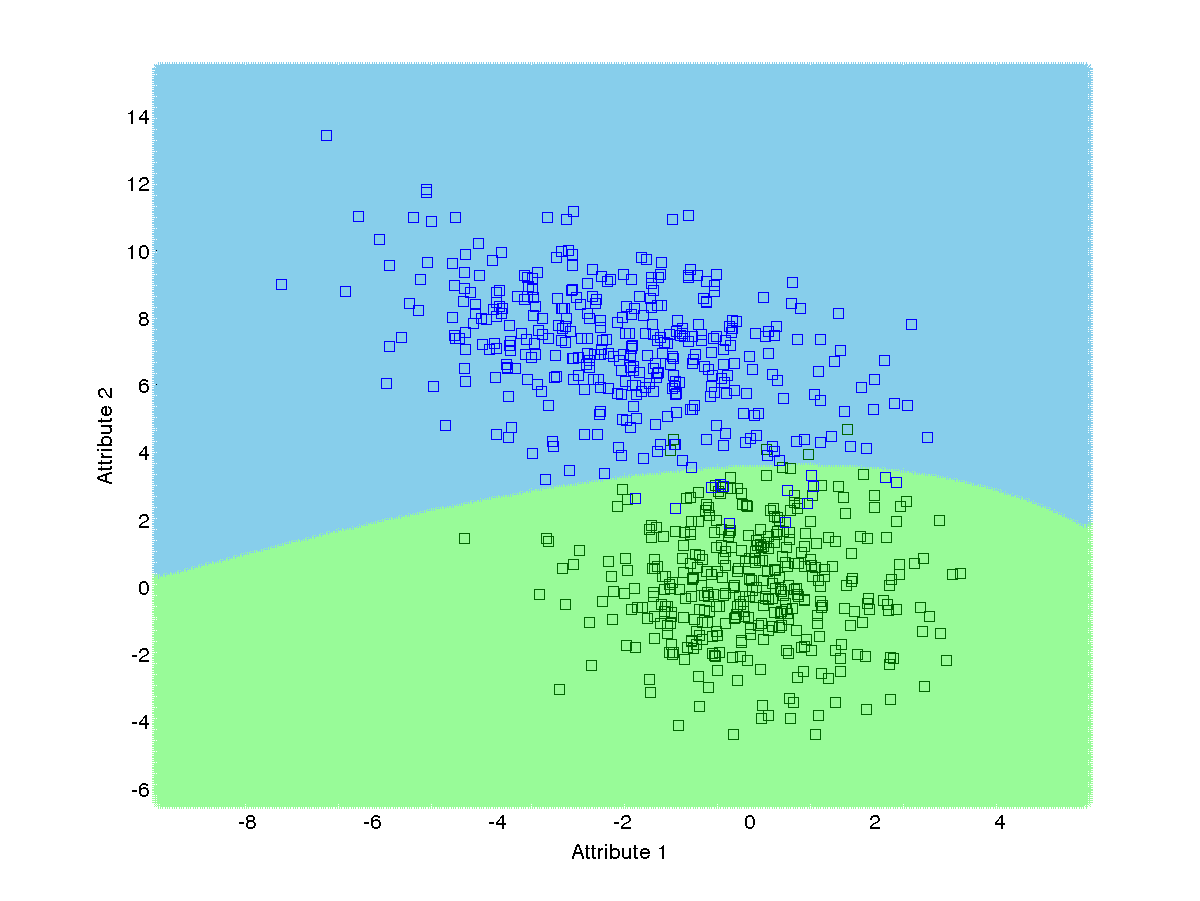
\includegraphics[width=40mm,height=30mm]{bayes/over/pair/14/diff_cov.png}\\
				\hline
				2 and
				3&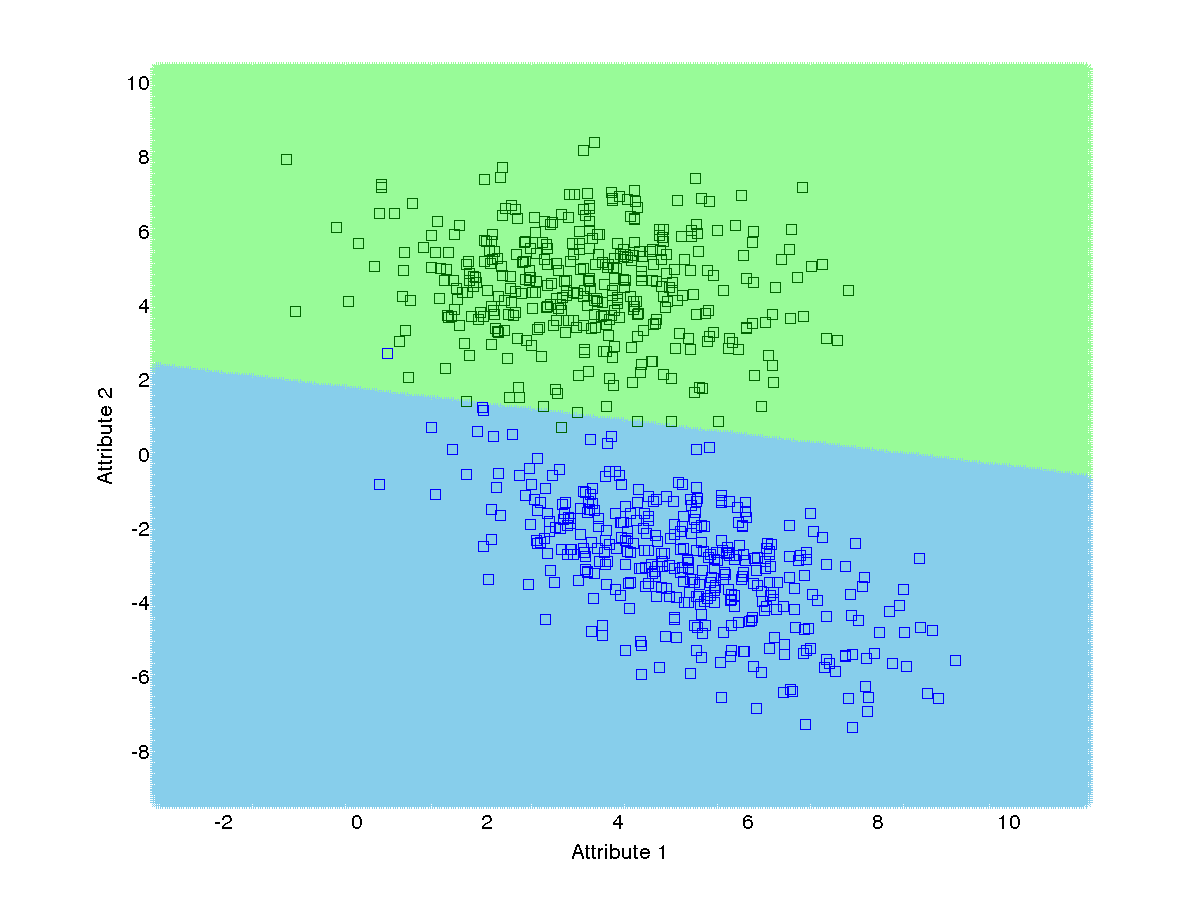
\includegraphics[width=40mm,height=30mm]{bayes/over/pair/23/all_cov.png}&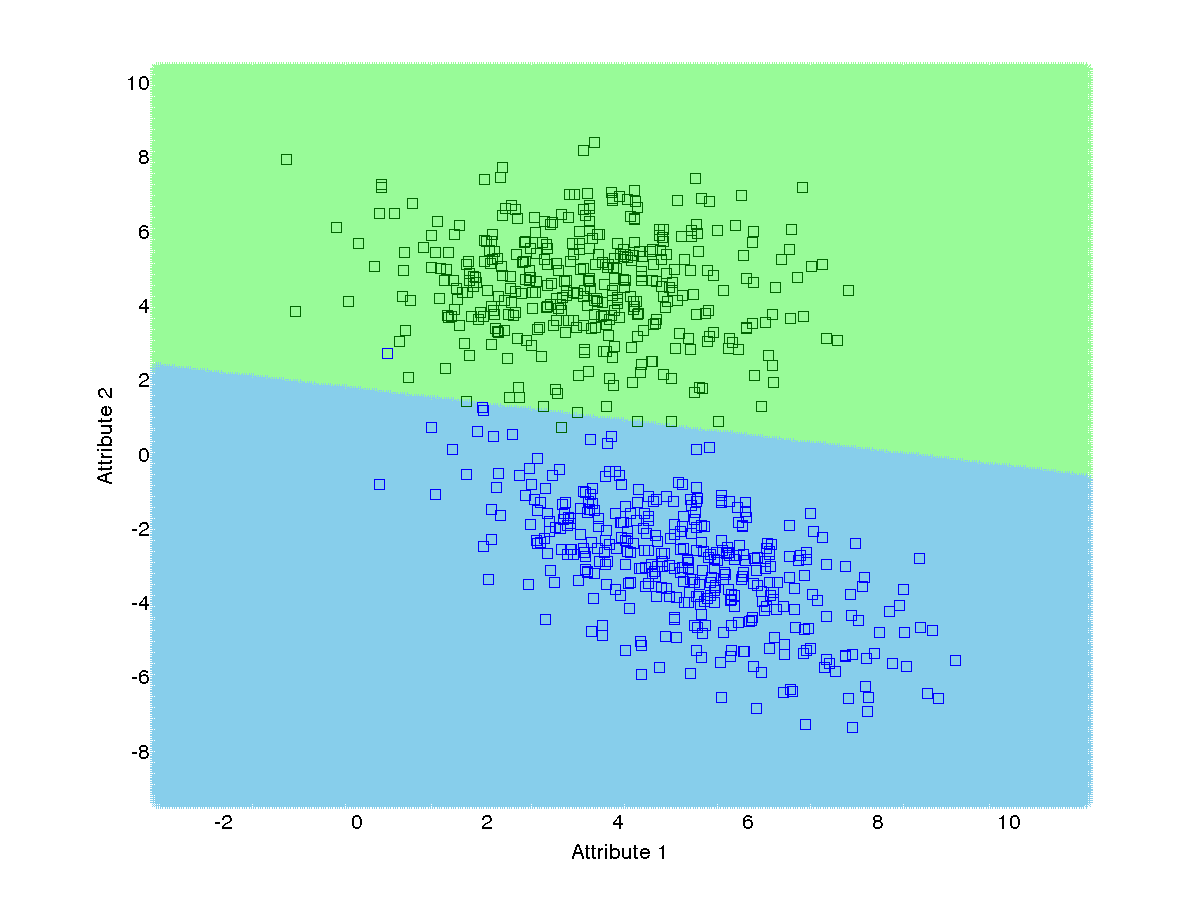
\includegraphics[width=40mm,height=30mm]{bayes/over/pair/23/avg_cov.png}
				&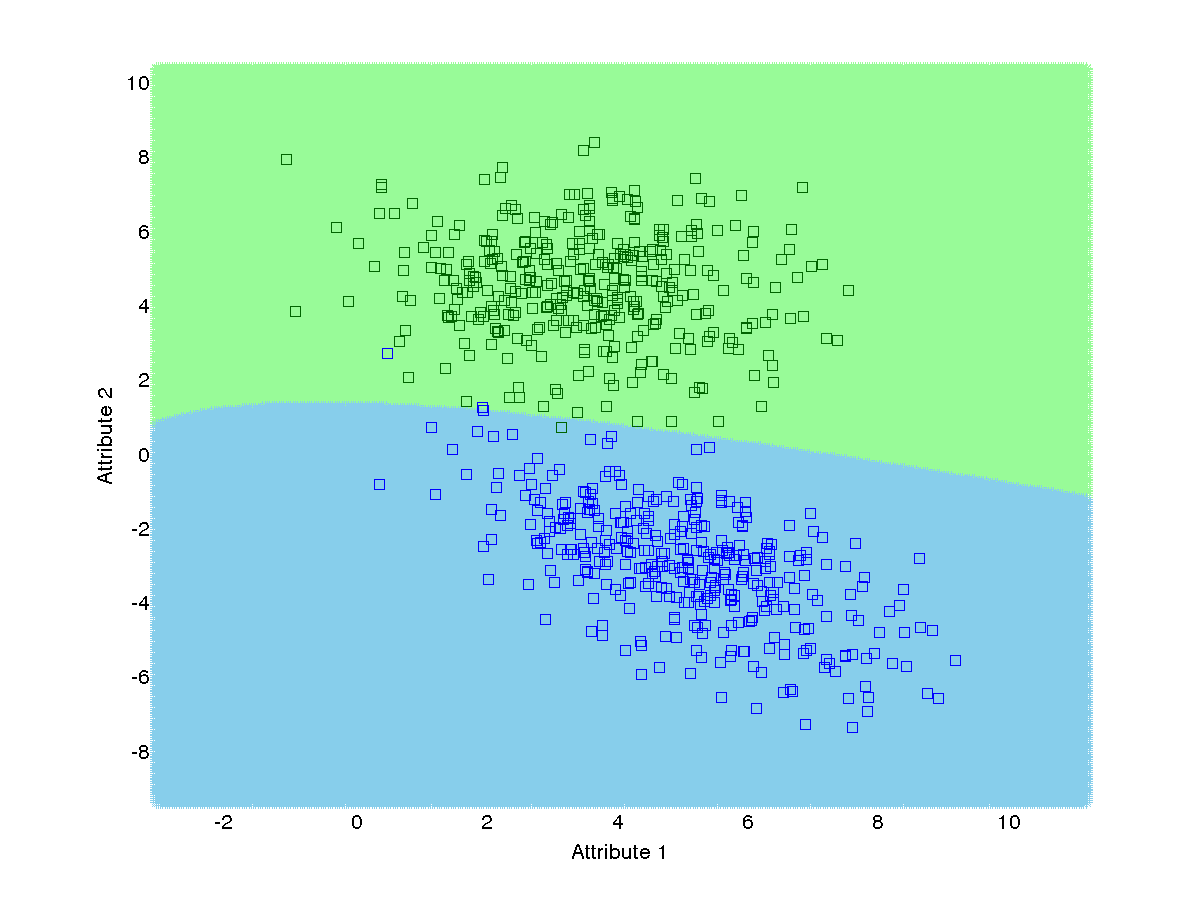
\includegraphics[width=40mm,height=30mm]{bayes/over/pair/23/diff_cov.png}\\
				\hline
				2 and
				4&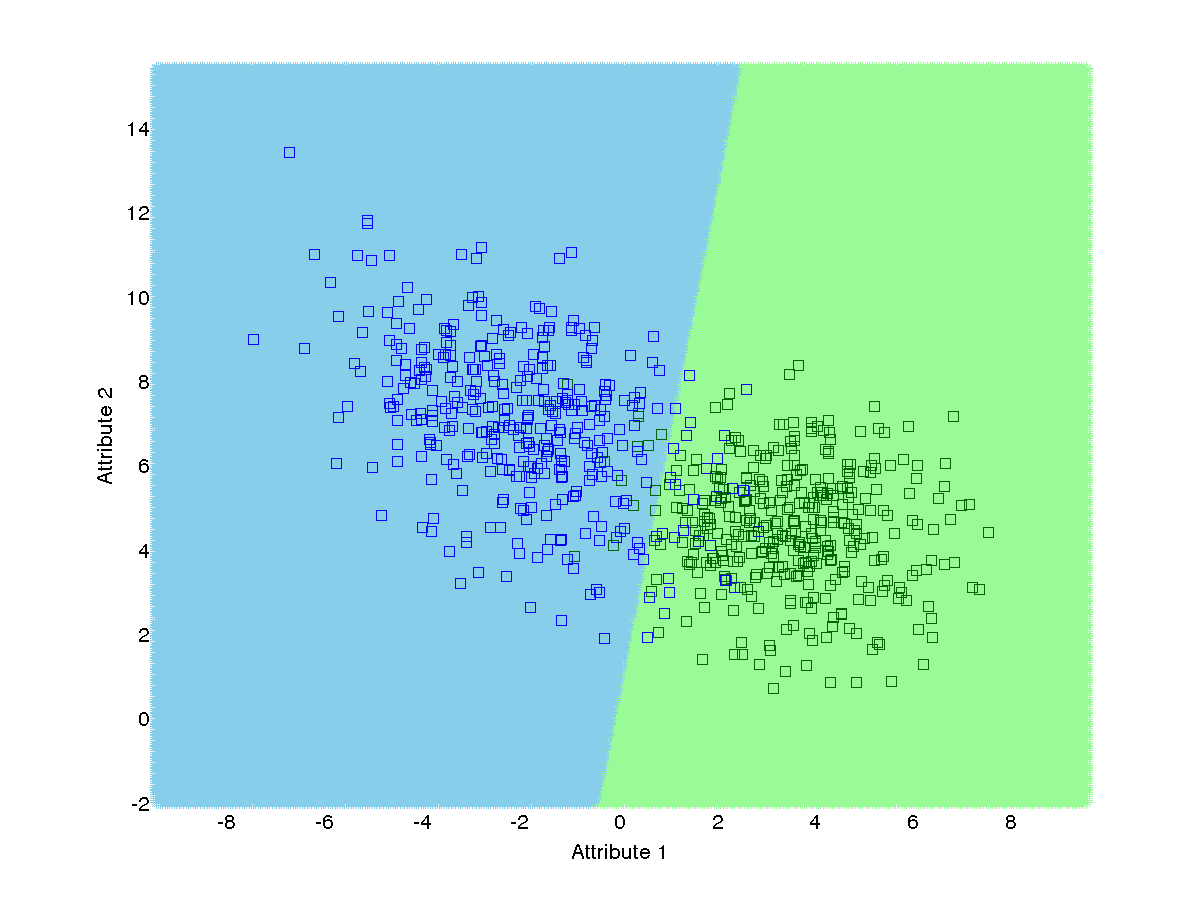
\includegraphics[width=40mm,height=30mm]{bayes/over/pair/24/all_cov.png}&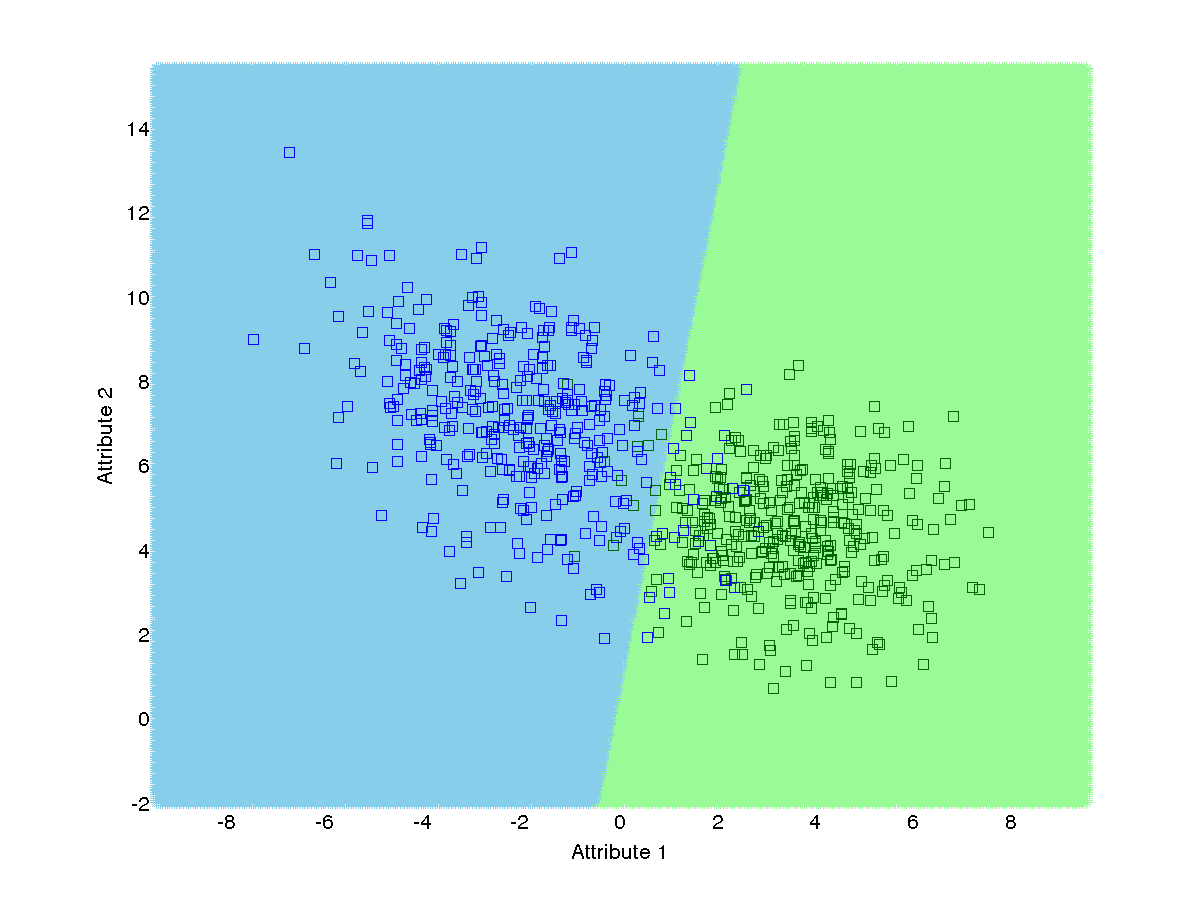
\includegraphics[width=40mm,height=30mm]{bayes/over/pair/24/avg_cov.png}
				&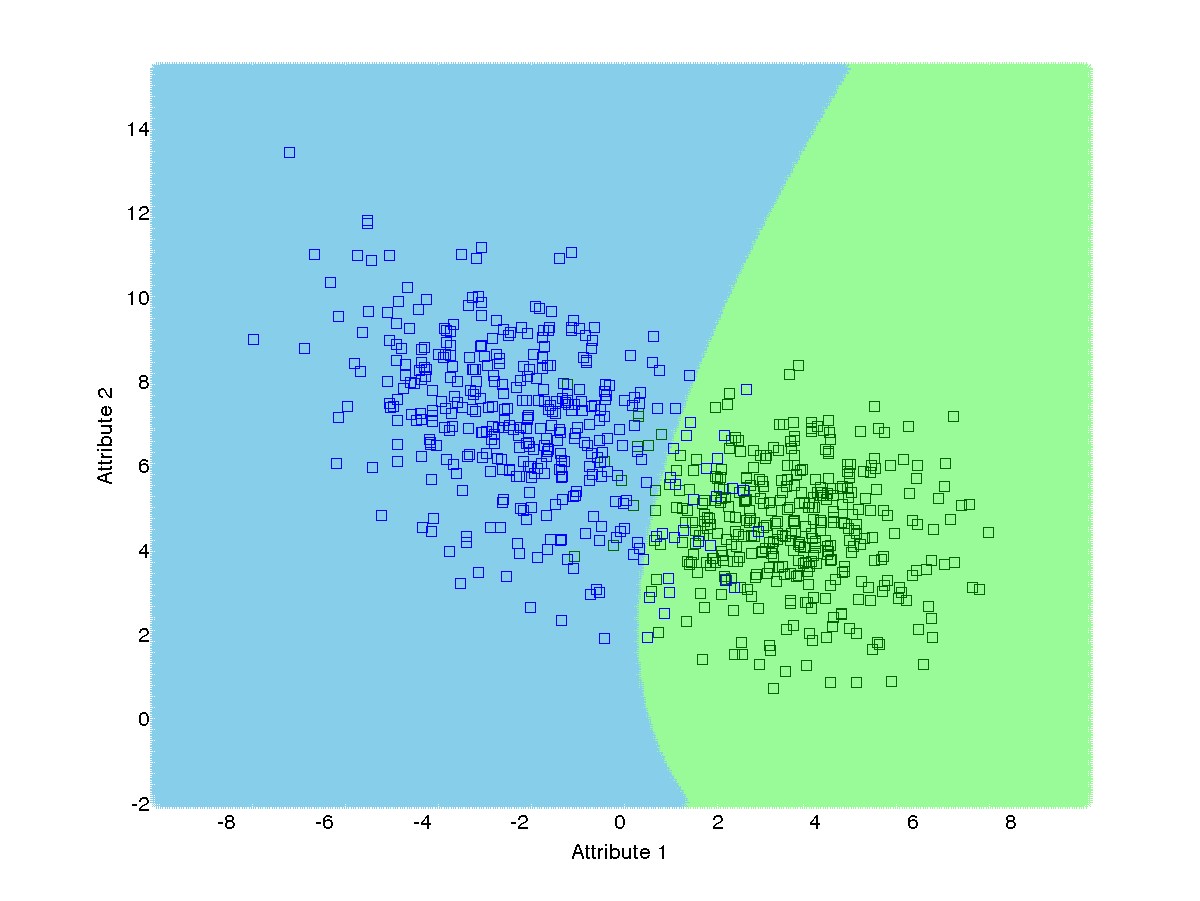
\includegraphics[width=40mm,height=30mm]{bayes/over/pair/24/diff_cov.png}\\
				\hline
				3 and
				4&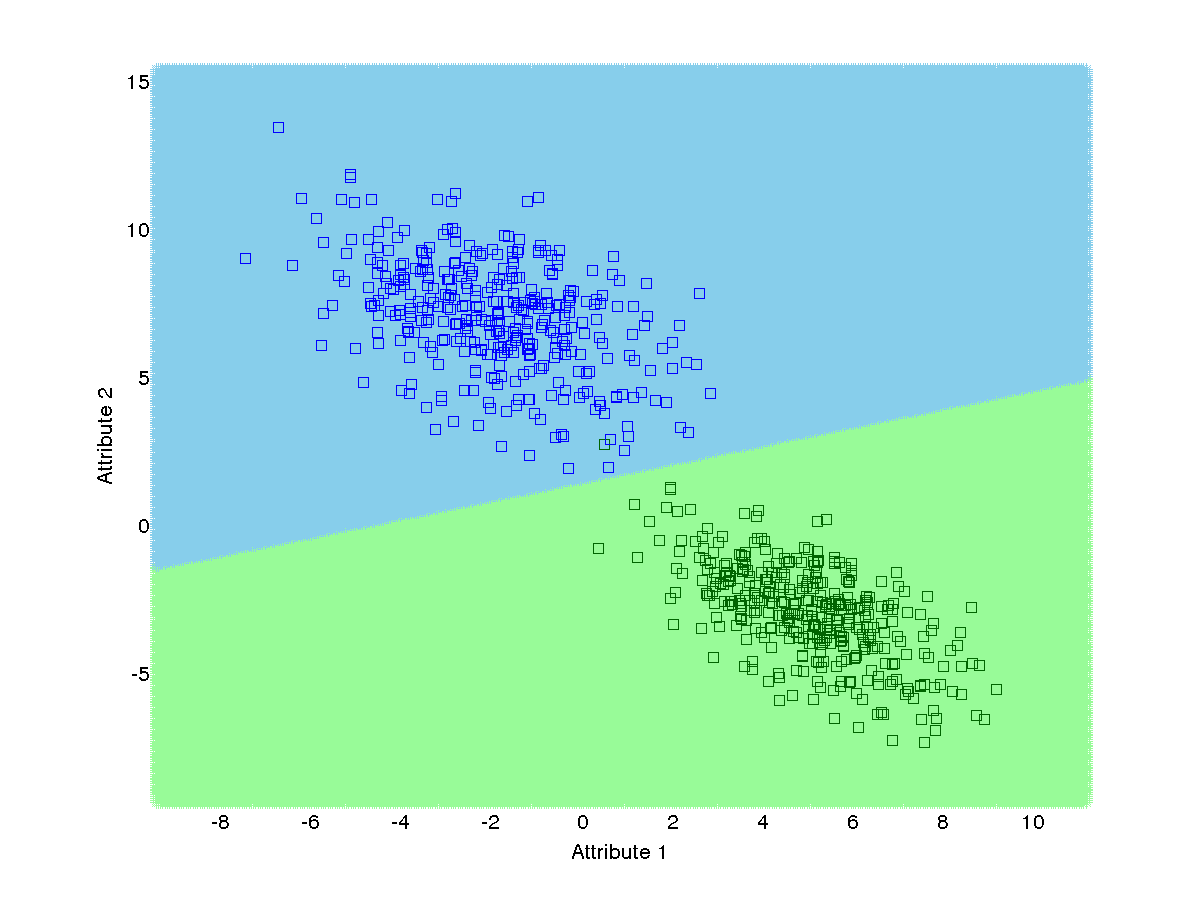
\includegraphics[width=40mm,height=30mm]{bayes/over/pair/34/all_cov.png}&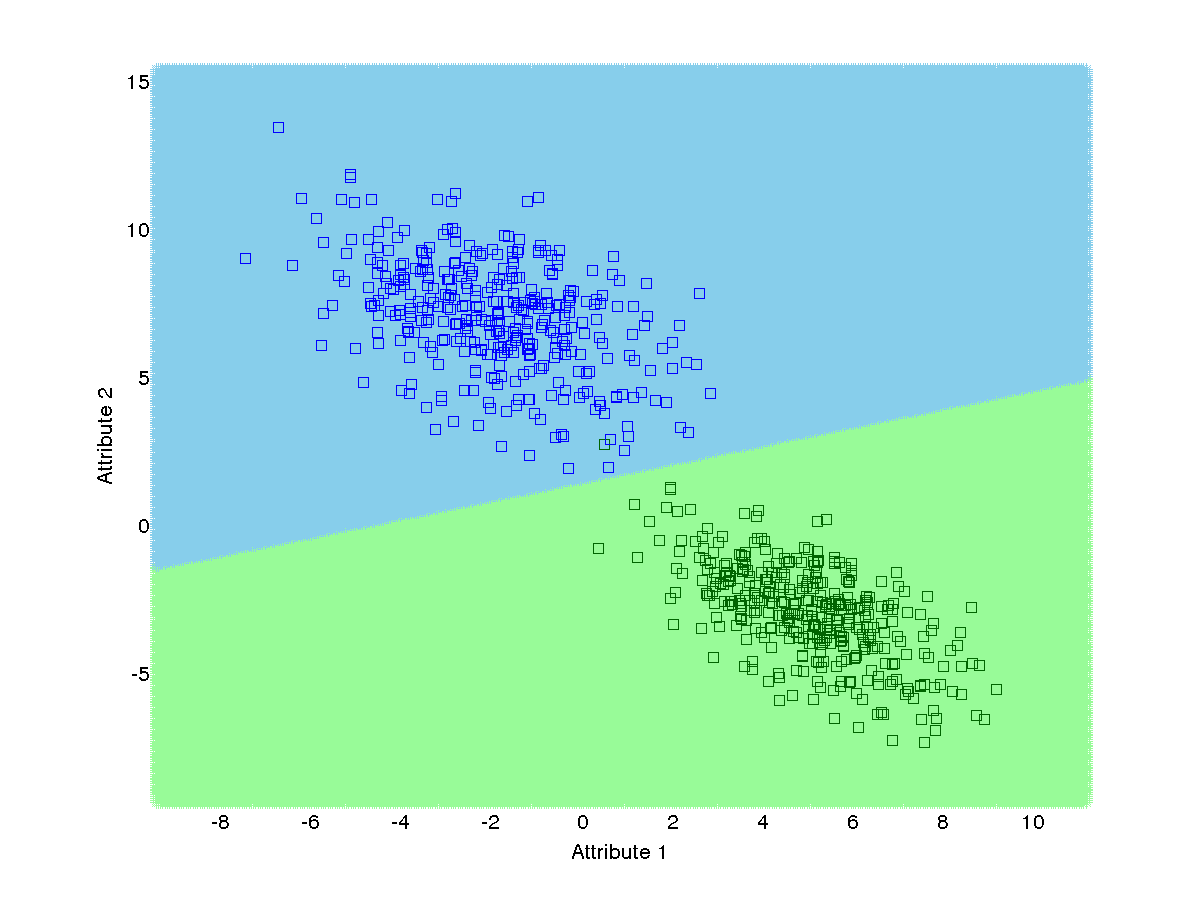
\includegraphics[width=40mm,height=30mm]{bayes/over/pair/34/avg_cov.png}
				&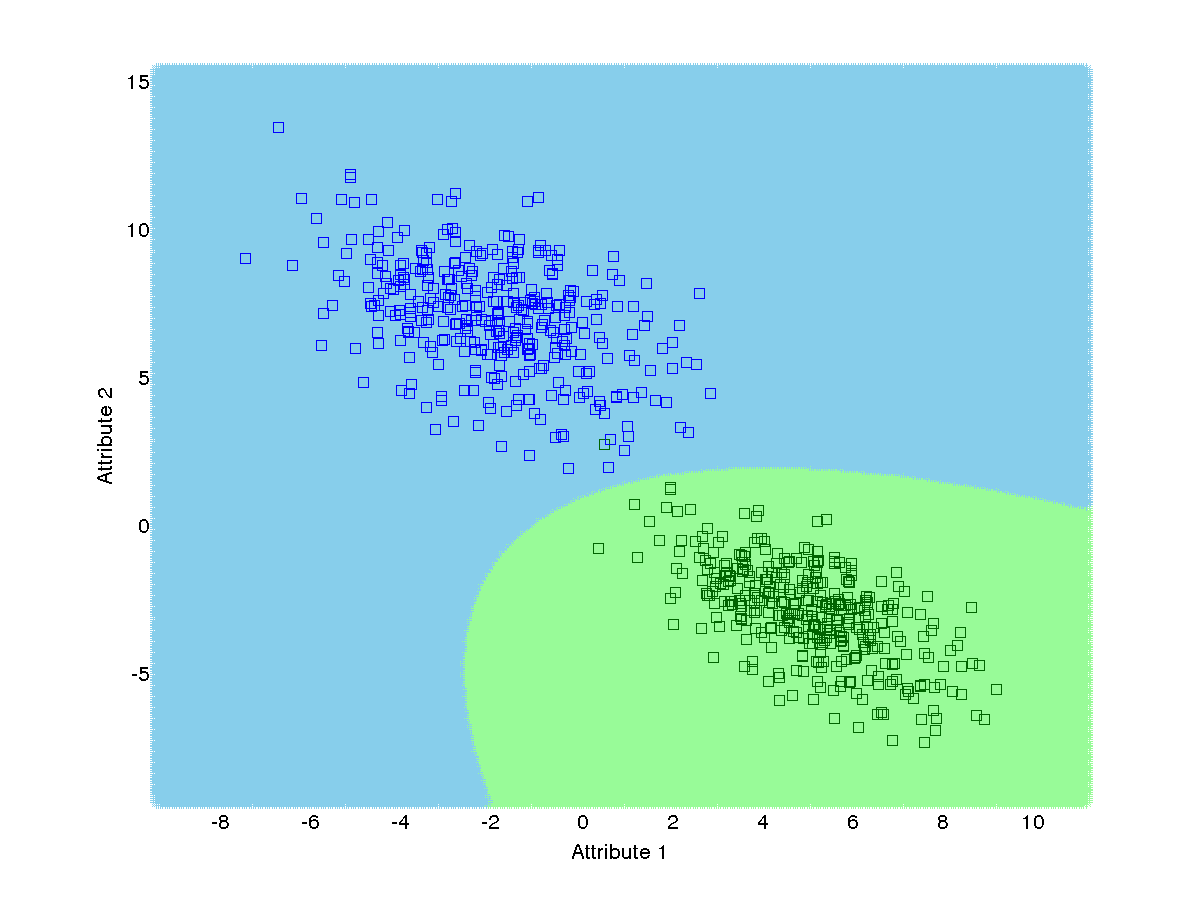
\includegraphics[width=40mm,height=30mm]{bayes/over/pair/34/diff_cov.png}\\
				\hline
				
			\end{tabular}
			\caption{Decision region plot for every pair of classes}
			\end{figure}
		
			
		
			\begin{minipage}[t]{0.6\linewidth}
			\vspace{0pt} % [3]
			  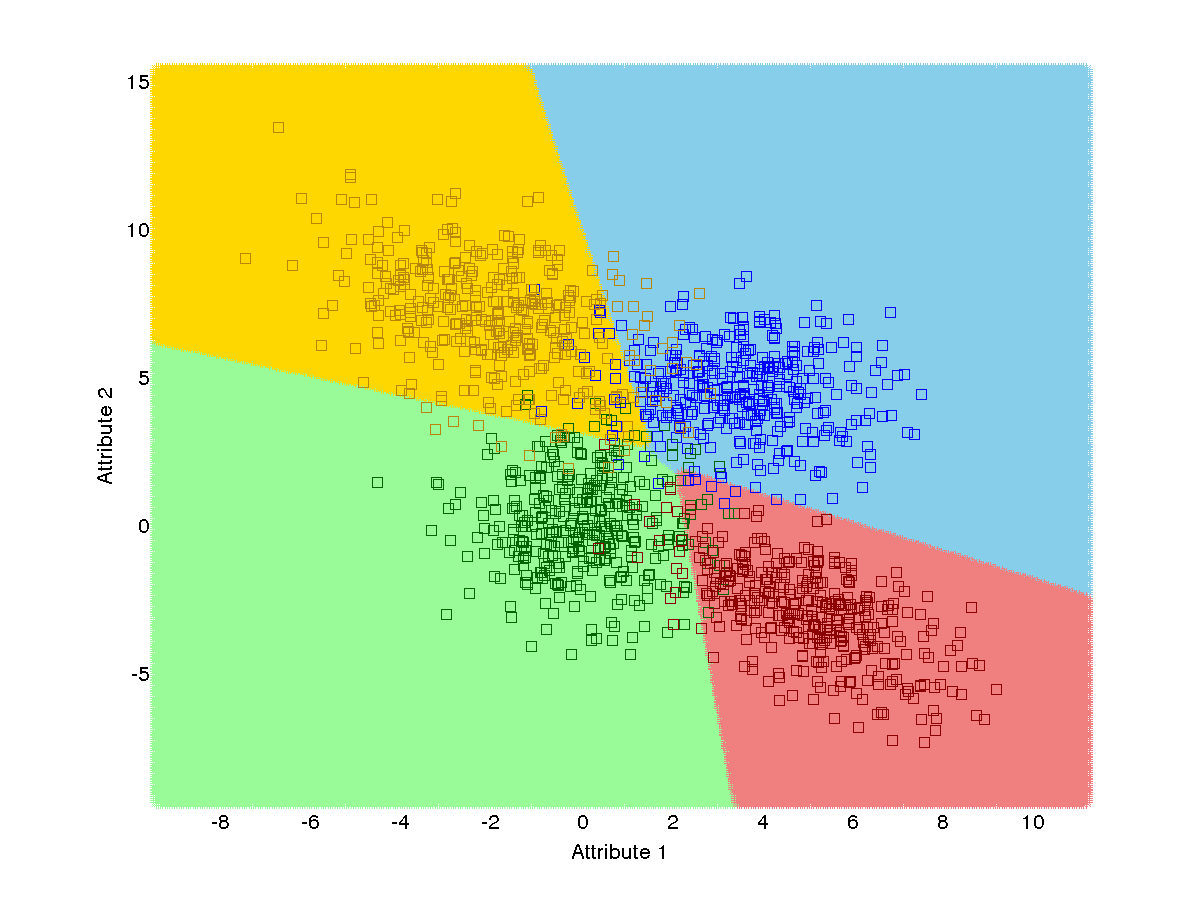
\includegraphics[width=\textwidth]{bayes/over/all/all_cov.png}
			  \captionof{figure}{ Decision region plot for all the classes together with the training data
 superposed with alltogether covariance} % [4]
			  \label{gfx/image}	
			\end{minipage}
			\begin{minipage}[t]{0.2\linewidth} % [2]
			\vspace{10pt} % [3]
				Correct   : 450	\\
				Incorrect : 50	\\
				Acurracy  : 90.000 \\
			\begin{center}
				\begin{tabular}{ |c|c|c|c|c|c| }
				\hline
				& & \multicolumn{4}{| c |}{Predicted} \\
				\hline
				& & Class 1 & Class 2 & Class 3 & Class 4\\
				\hline
				\multirow{4}{*}{\rotatebox[origin=c]{90}{Act.}} & Class 1& 111 & 4 & 4 & 6\\
				& Class 2 & 1 & 116 & 0 & 8\\
				& Class 3 & 9 & 0 & 116 & 0\\
				& Class 4 & 6 & 12 & 0 & 107\\
				\hline
				\end{tabular}
				\end{center}
			\end{minipage}
	
		\begin{minipage}[t]{0.6\linewidth}
			\vspace{0pt} % [3]
			  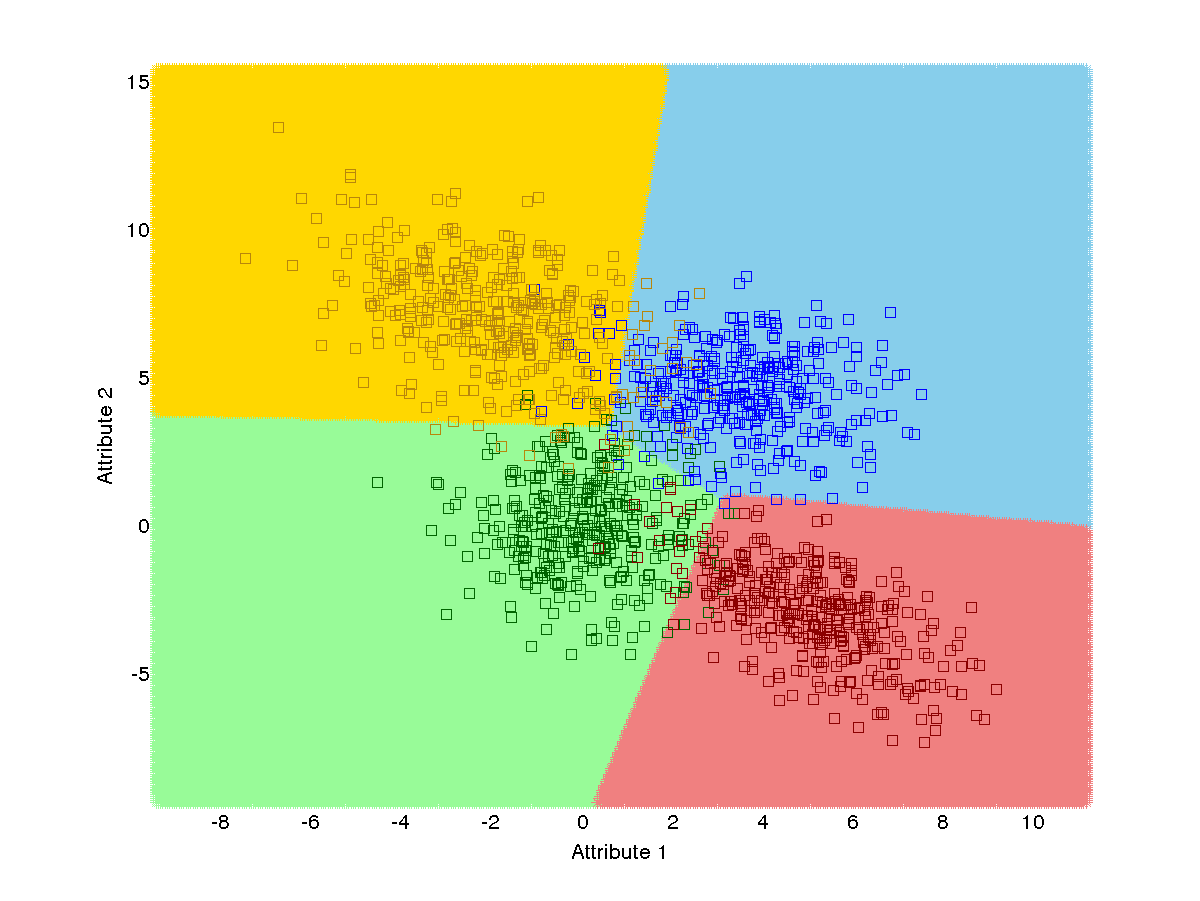
\includegraphics[width=\textwidth]{bayes/over/all/avg_cov.png}
			  \captionof{figure}{ Decision region plot for all the classes together with the training data
 superposed with average covariance} % [4]
			  \label{gfx/image}	
			\end{minipage}
			\begin{minipage}[t]{0.2\linewidth} % [2]
			\vspace{10pt} % [3]
				Correct   : 453	\\
				Incorrect : 47	\\
				Acurracy  : 90.600 \\
			\begin{center}
				\begin{tabular}{ |c|c|c|c|c|c| }
				\hline
				& & \multicolumn{4}{| c |}{Predicted} \\
				\hline
				& & Class 1 & Class 2 & Class 3 & Class 4\\
				\hline
				\multirow{4}{*}{\rotatebox[origin=c]{90}{Act.}} & Class 1& 111 & 6 & 4 & 4\\
				& Class 2 & 2 & 118 & 0 & 5\\
				& Class 3 &9 & 0 & 116 & 0\\
				& Class 4 & 5 & 12 & 0 & 108\\
				\hline
				\end{tabular}
				\end{center}
			\end{minipage}
			
		\begin{minipage}[t]{0.6\linewidth}
			\vspace{0pt} % [3]
			  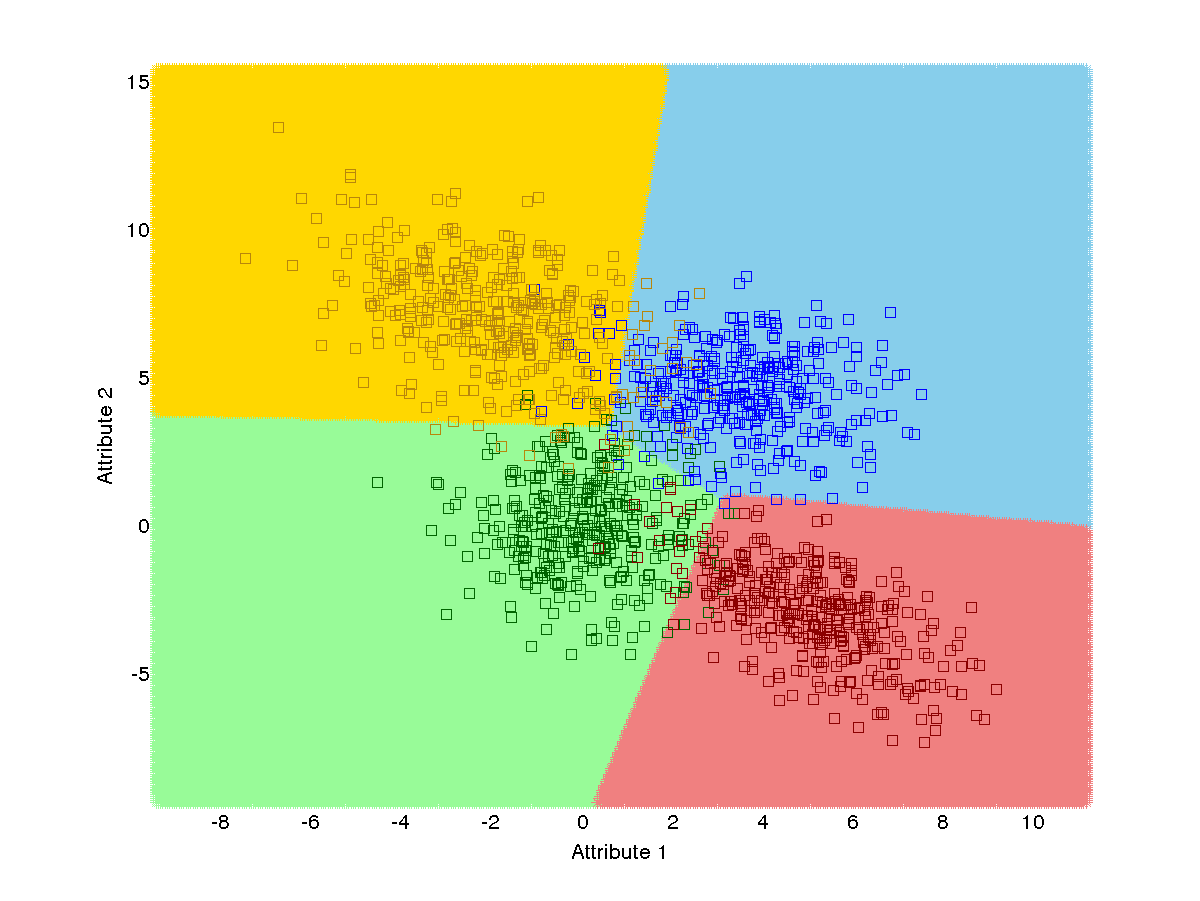
\includegraphics[width=\textwidth]{bayes/over/all/avg_cov.png}
			  \captionof{figure}{ Decision region plot for all the classes together with the training data
 superposed with different covariance} % [4]
			  \label{gfx/image}	
			\end{minipage}
			\begin{minipage}[t]{0.2\linewidth} % [2]
			\vspace{10pt} % [3]
				Correct   : 452	\\
				Incorrect : 48	\\
				Acurracy  : 90.400 \\
			\begin{center}
				\begin{tabular}{ |c|c|c|c|c|c| }
				\hline
				& & \multicolumn{4}{| c |}{Predicted} \\
				\hline
				& & Class 1 & Class 2 & Class 3 & Class 4\\
				\hline
				\multirow{4}{*}{\rotatebox[origin=c]{90}{Act.}} & Class 1& 113 & 4 & 4 & 4\\
				& Class 2 & 2 & 118 & 0 & 5\\
				& Class 3 & 12 & 0 & 113 & 0\\
				& Class 4 & 5 & 12 & 0 & 108\\
				\hline
				\end{tabular}
				\end{center}
			\end{minipage}
			
	
		%%%%%%%%%%%%%%%%%%%%%%%%%%%%%%%%%%%%%%%%%%%%%%%%%%%%%%%%%5
		\subsubsection{Real world data set}
			
	
		\begin{minipage}[t]{0.6\linewidth}
			\vspace{0pt} % [3]
			 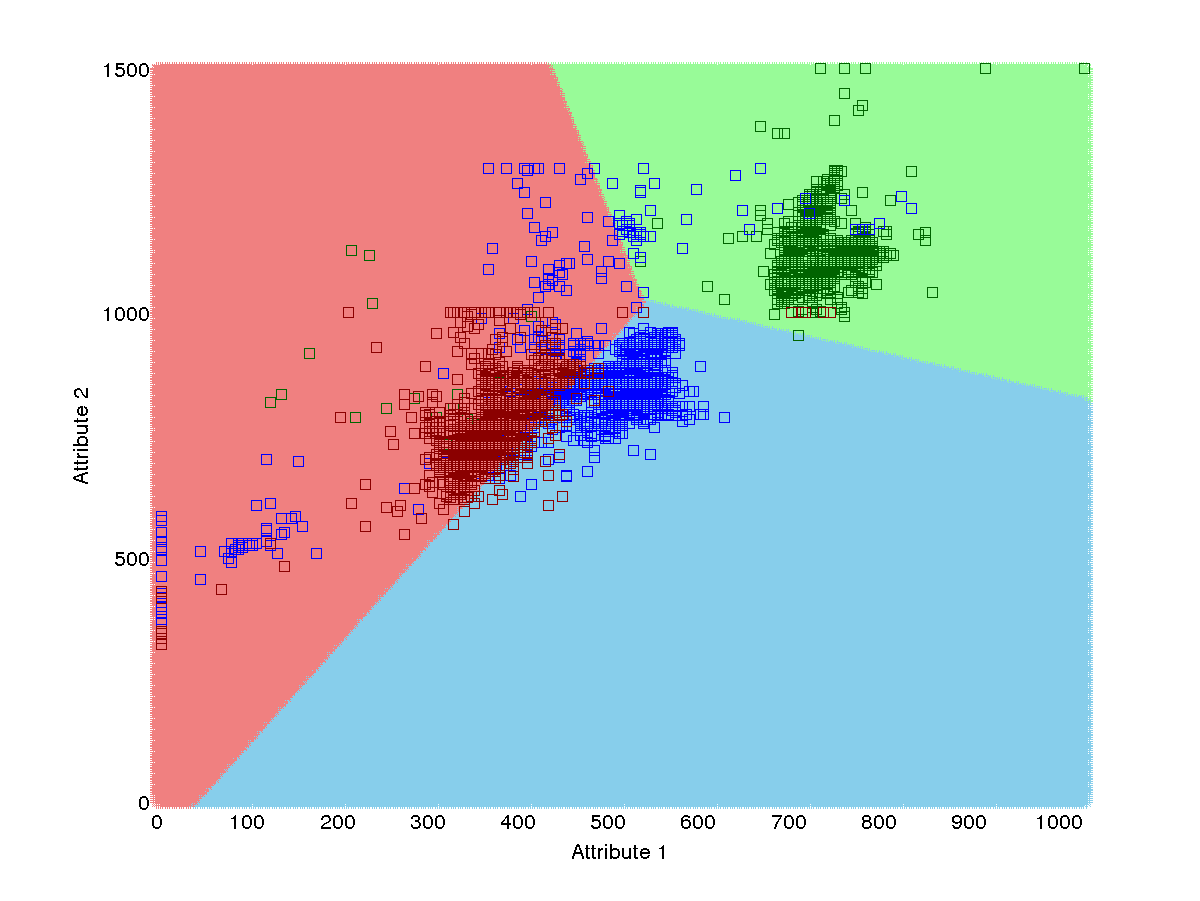
\includegraphics[width=\textwidth]{bayes/real/all/all_cov.png}
		  	\captionof{figure}{ Decision region plot for all the classes together with the training data
superposed with alltogether covariance} % [4]
		  \label{gfx/image}	
		\end{minipage}
		\begin{minipage}[t]{0.2\linewidth} % [2]
		\vspace{10pt} % [3]
			Correct   : 1386	\\
			Incorrect : 391	\\
			Acurracy  : 77.9966 \\
		\begin{center}
			\begin{tabular}{ |c|c|c|c|c| }
			\hline
			& & \multicolumn{3}{| c |}{Predicted} \\
			\hline
			& & Class 1 & Class 2 & Class 3\\
			\hline
			\multirow{3}{*}{\rotatebox[origin=c]{90}{Act.}} & Class 1 & 510 & 1 & 30\\
			& Class 2 & 21 & 332 & 261\\
			& Class 3 & 7 & 71 & 544\\
			\hline
			\end{tabular}
			\end{center}
		\end{minipage}
	
		\begin{minipage}[t]{0.6\linewidth}
			\vspace{0pt} % [3]
			  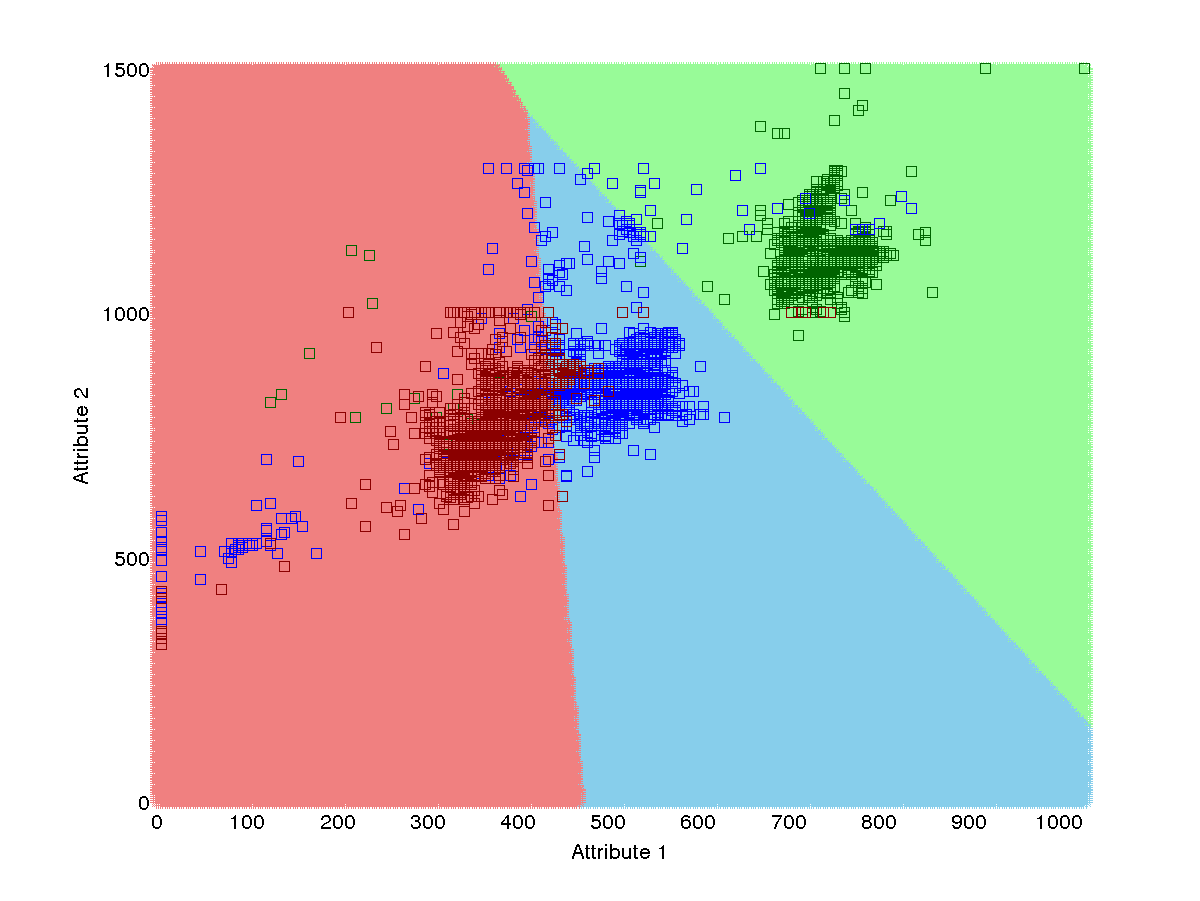
\includegraphics[width=\textwidth]{bayes/real/all/avg_cov.png}
			  \captionof{figure}{ Decision region plot for all the classes together with the training data
 superposed with average covariance} % [4]
			  \label{gfx/image}	
			\end{minipage}
			\begin{minipage}[t]{0.2\linewidth} % [2]
			\vspace{10pt} % [3]
				Correct   : 1509	\\
				Incorrect : 268	\\
				Acurracy  :	84.9184 \\
			\begin{center}
				\begin{tabular}{ |c|c|c|c|c| }
				\hline
				& & \multicolumn{3}{| c |}{Predicted} \\
				\hline
				& & Class 1 & Class 2 & Class 3\\
				\hline
				\multirow{3}{*}{\rotatebox[origin=c]{90}{Act.}} & Class 1 & 510 & 5 & 26\\
				& Class 2 & 20 & 397 & 197\\
				& Class 3 & 7 & 13 & 602\\
				\hline
				\end{tabular}
				\end{center}
			\end{minipage}
			
		\begin{minipage}[t]{0.6\linewidth}
			\vspace{0pt} % [3]
			  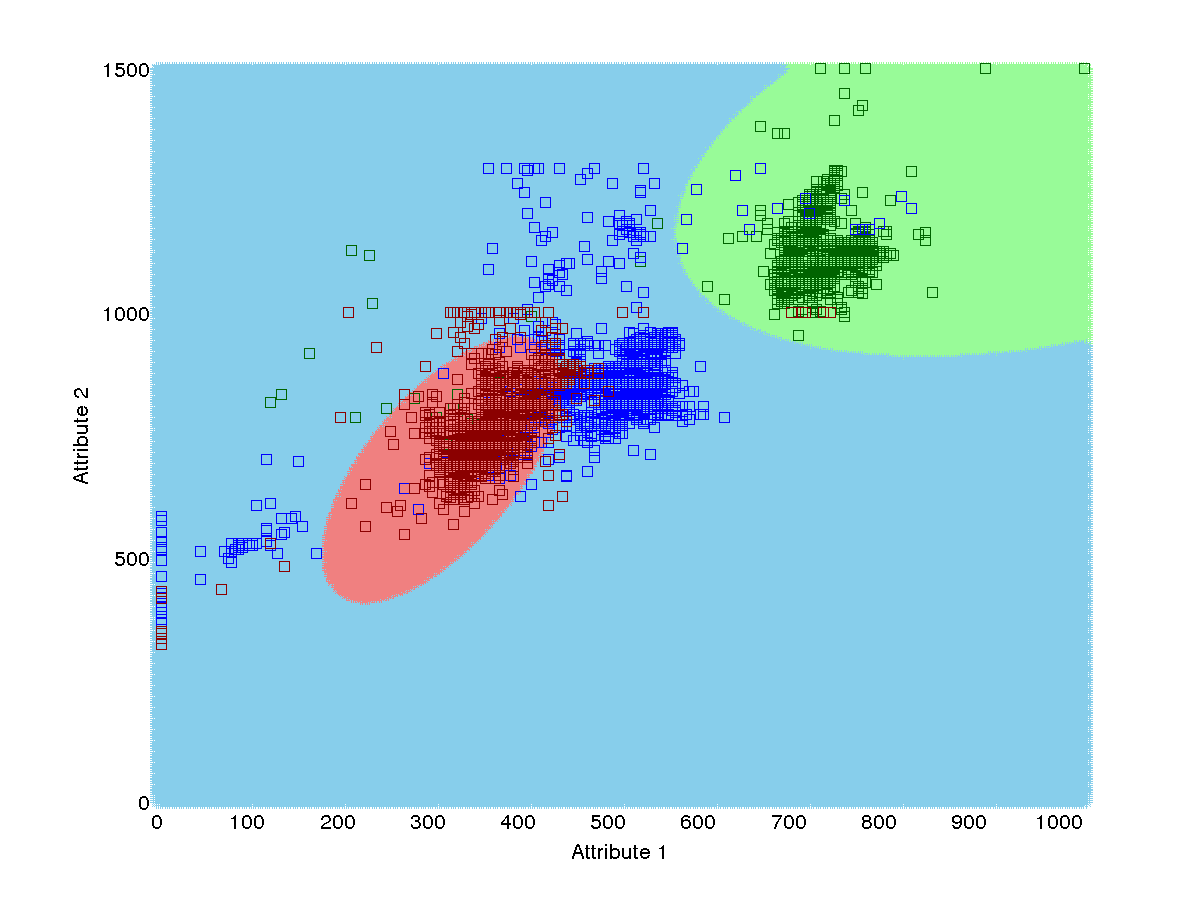
\includegraphics[width=\textwidth]{bayes/real/all/diff_cov.png}
			  \captionof{figure}{ Decision region plot for all the classes together with the training data
 superposed with different covariance} % [4]
			  \label{gfx/image}	
			\end{minipage}
			\begin{minipage}[t]{0.2\linewidth} % [2]
			\vspace{10pt} % [3]
				Correct   : 375	\\
				Incorrect : 0	\\
				Acurracy  : 100 \\
			\begin{center}
				\begin{tabular}{ |c|c|c|c|c| }
				\hline
				& & \multicolumn{3}{| c |}{Predicted} \\
				\hline
				& & Class 1 & Class 2 & Class 3\\
				\hline
				\multirow{3}{*}{\rotatebox[origin=c]{90}{Act.}} & Class 1 & 125 & 0 & 0\\
				& Class 2 & 0 & 125 & 0\\
				& Class 3 & 0 & 0 & 125\\
				\hline
				\end{tabular}
				\end{center}
			\end{minipage}
			
	
		
		%%%%%%%%%%%%%%%%%%%%%%%%%%%%%%%%%%%%%%%%%%%%%%%%%%%%%%%%%5
			
			\begin{figure}
				\begin{tabular}{|c|c|c|c|}
					\hline
					Pair/Cov &  Alltogther & Average & Different	\\
					\hline
					1 and
					2&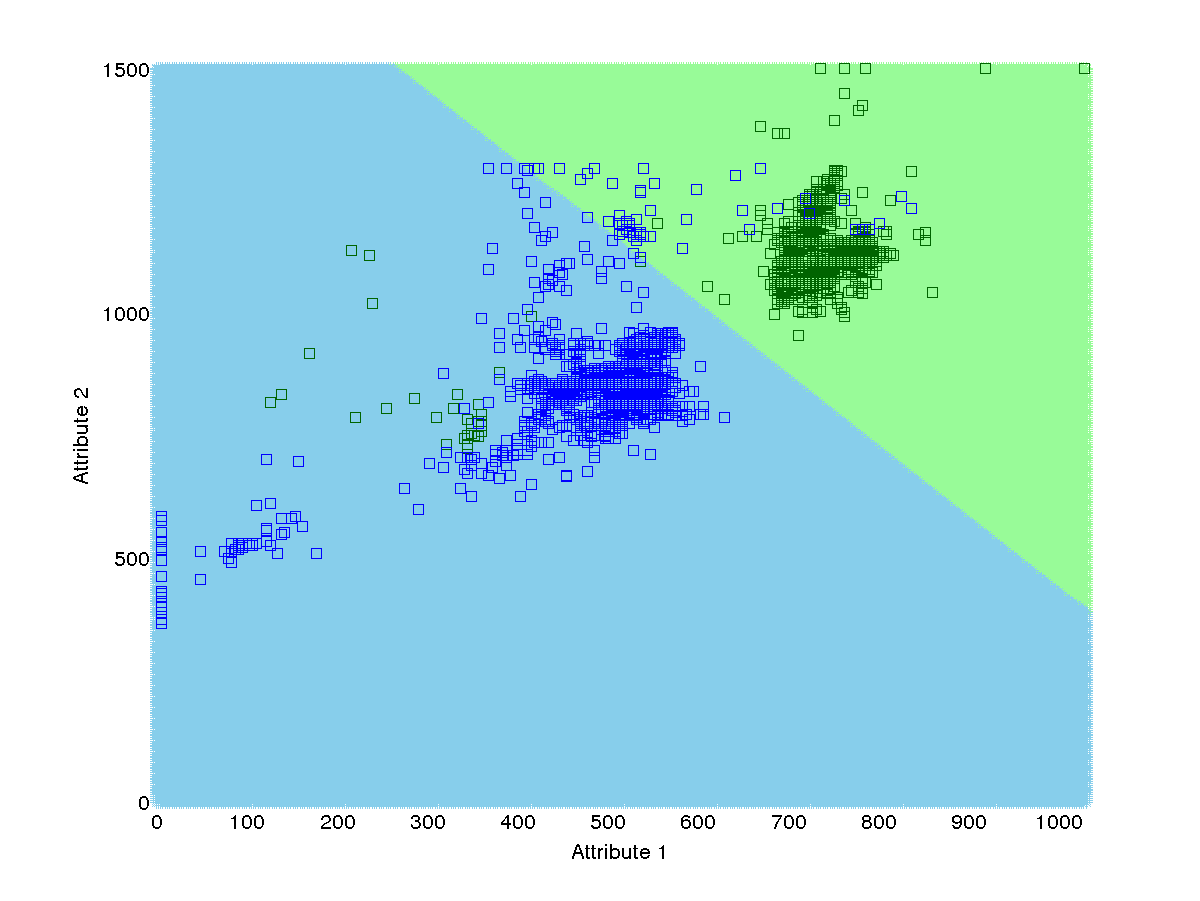
\includegraphics[width=40mm,height=30mm]{bayes/real/pair/12/all_cov.png}&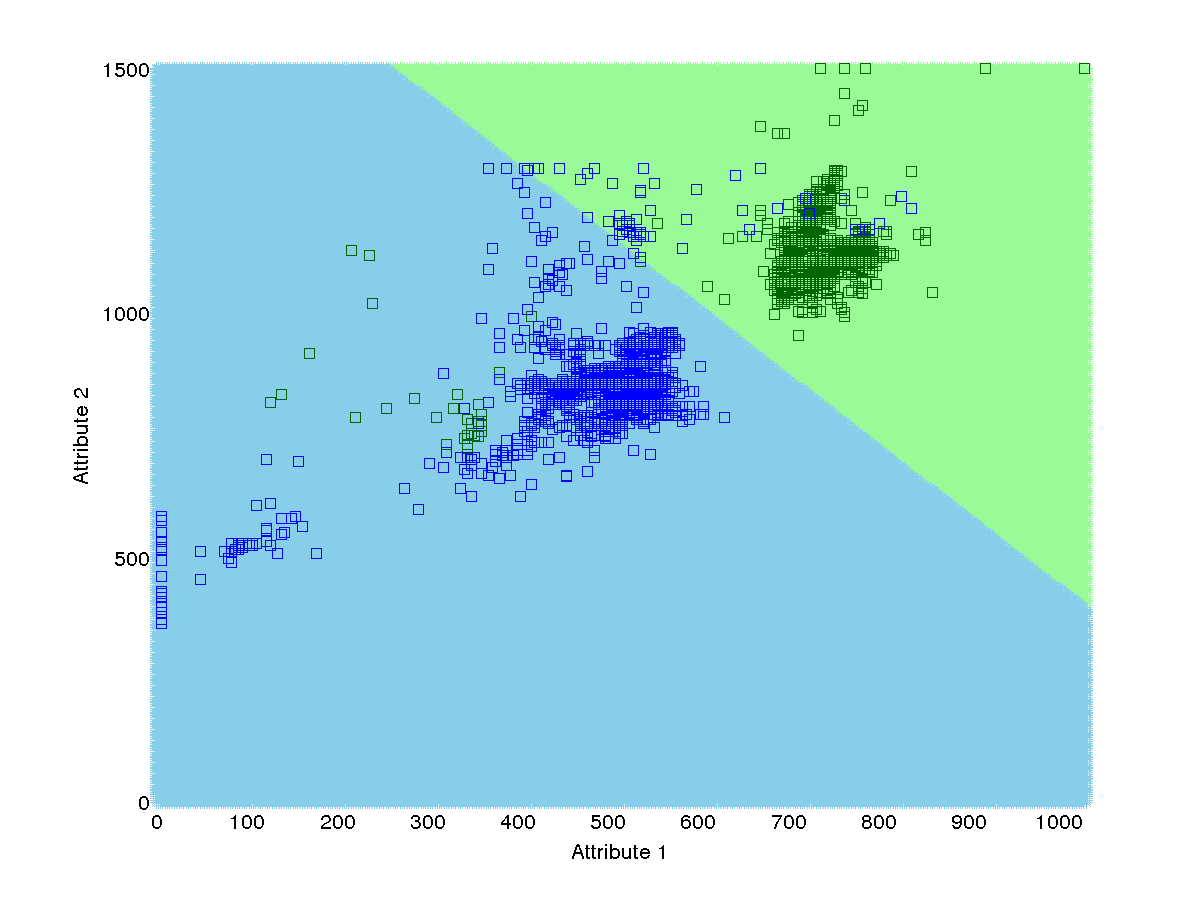
\includegraphics[width=40mm,height=30mm]{bayes/real/pair/12/avg_cov.png}
					&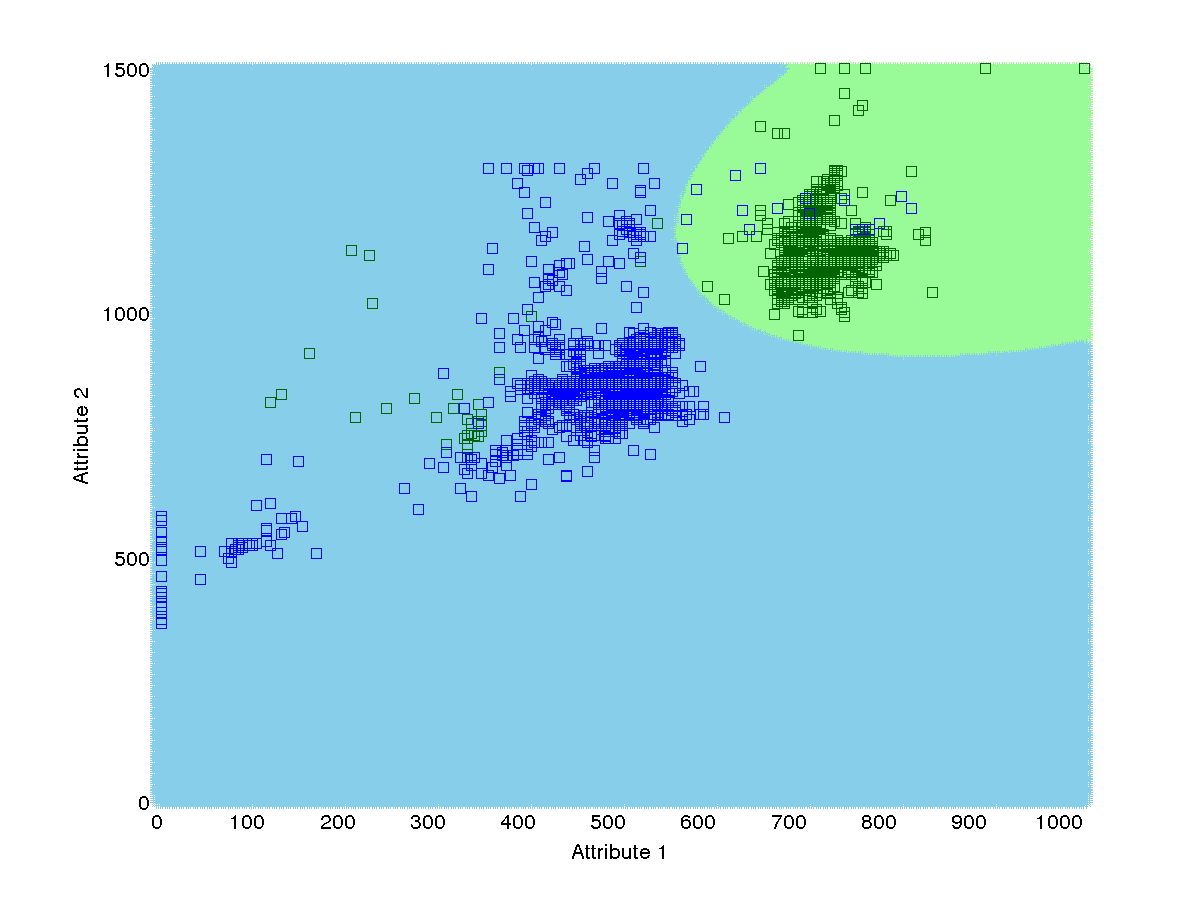
\includegraphics[width=40mm,height=30mm]{bayes/real/pair/12/diff_cov.png}\\
					\hline
					1 and
					3&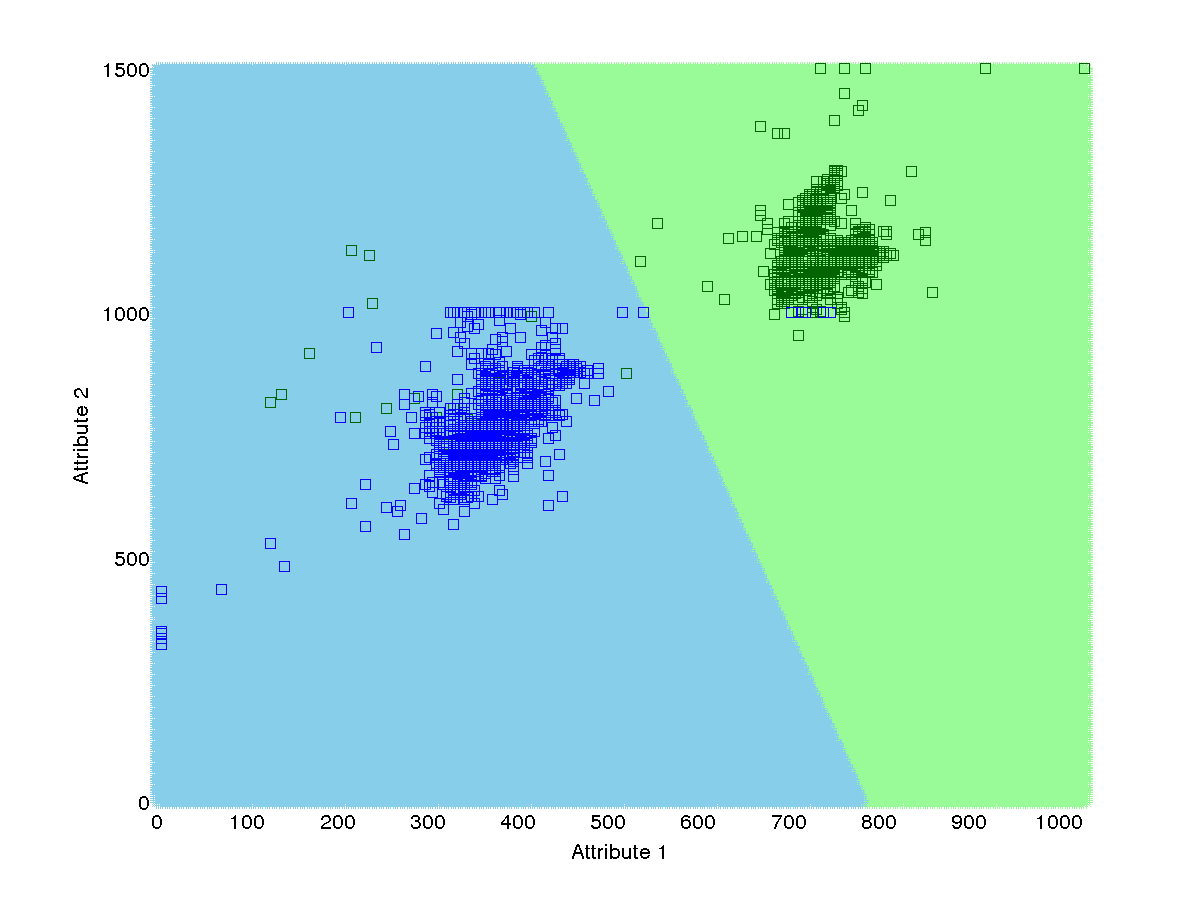
\includegraphics[width=40mm,height=30mm]{bayes/real/pair/13/all_cov.png}&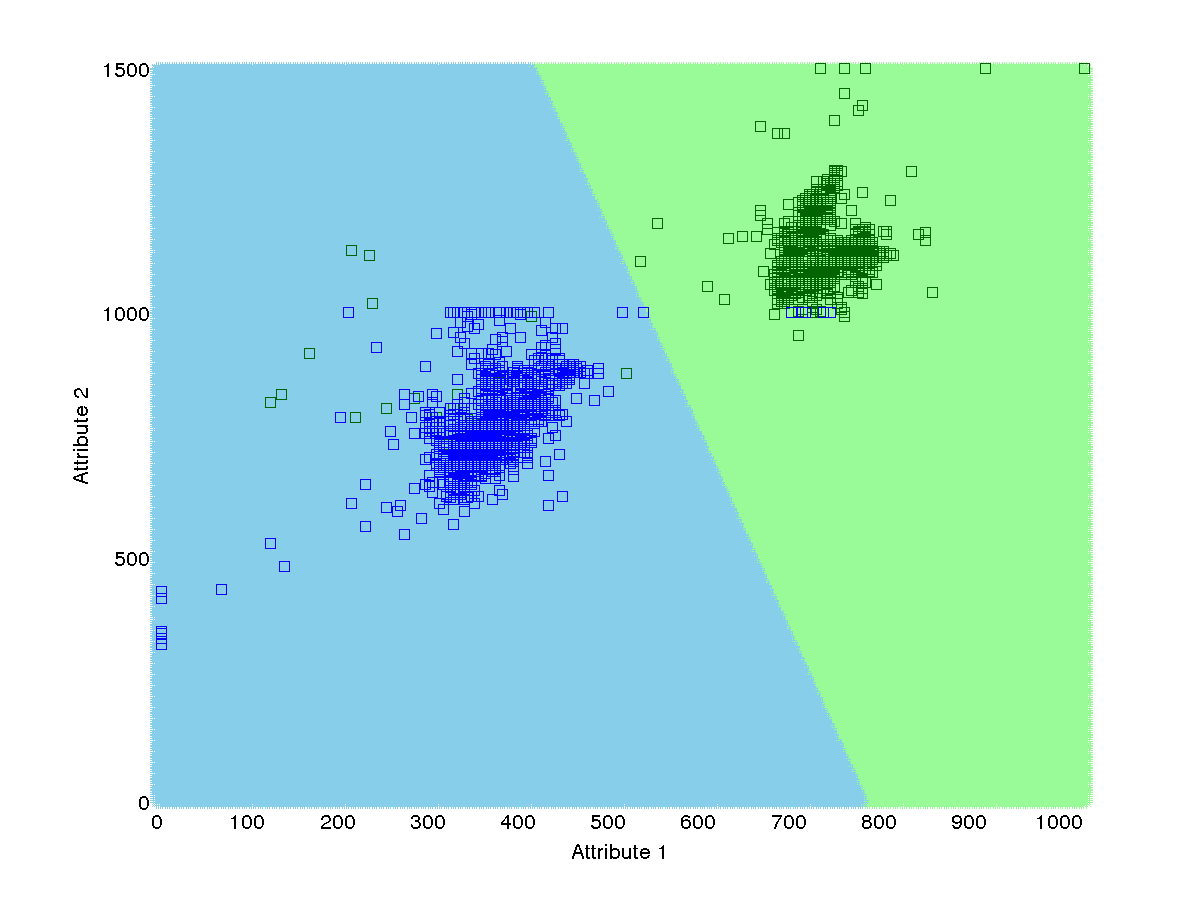
\includegraphics[width=40mm,height=30mm]{bayes/real/pair/13/all_cov.png}
					&\includegraphics[width=40mm,height=30mm]{bayes/real/pair/13/diff_cov.png}\\
					\hline
					2 and
					3&\includegraphics[width=40mm,height=30mm]{bayes/real/pair/23/all_cov.png}&\includegraphics[width=40mm,height=30mm]{bayes/real/pair/23/avg_cov.png}
					&\includegraphics[width=40mm,height=30mm]{bayes/real/pair/23/diff_cov.png}\\
					\hline
				\end{tabular}
				\caption{Decision region plot for every pair of classes}
			\end{figure}
	
		%%%%%%%%%%%%%%%%%%%%%%%%%%%%%%%%%%%%%%%%%%%%%%%%%%%%%%%%%5

	\subsection{Naive-Bayes classifier}

			\subsubsection{Linearly separable data set}
				%%%%%%%%%%%%%%%%%%%%%%%%%%%%%%%%%%%%%%%%%%%%%%%%%%%%%%%%%5
			
			\
		
			
		
		\begin{minipage}[t]{0.6\linewidth}
			\vspace{0pt} % [3]
			 \includegraphics[width=\textwidth]{naivebayes/ls/all/all_cov.png}
		  	\captionof{figure}{ Decision region plot for all the classes together with the training data
superposed with alltogether covariance} % [4]
		  \label{gfx/image}	
		\end{minipage}
		\begin{minipage}[t]{0.2\linewidth} % [2]
		\vspace{10pt} % [3]
			Correct   : 374	\\
			Incorrect : 1	\\
			Acurracy  : 99.733 \\
		\begin{center}
			\begin{tabular}{ |c|c|c|c|c| }
			\hline
			& & \multicolumn{3}{| c |}{Predicted} \\
			\hline
			& & Class 1 & Class 2 & Class 3\\
			\hline
			\multirow{3}{*}{\rotatebox[origin=c]{90}{Act.}} & Class 1 & 125 & 0 & 0\\
			& Class 2 & 0 & 125 & 0\\
			& Class 3 & 0 & 1 & 124\\
			\hline
			\end{tabular}
			\end{center}
		\end{minipage}
	
		\begin{minipage}[t]{0.6\linewidth}
			\vspace{0pt} % [3]
			  \includegraphics[width=\textwidth]{naivebayes/ls/all/avg_cov.png}
			  \captionof{figure}{ Decision region plot for all the classes together with the training data
 superposed with average covariance} % [4]
			  \label{gfx/image}	
			\end{minipage}
			\begin{minipage}[t]{0.2\linewidth} % [2]
			\vspace{10pt} % [3]
				Correct   : 374	\\
				Incorrect : 1	\\
				Acurracy  : 99.733 \\
			\begin{center}
				\begin{tabular}{ |c|c|c|c|c| }
				\hline
				& & \multicolumn{3}{| c |}{Predicted} \\
				\hline
				& & Class 1 & Class 2 & Class 3\\
				\hline
				\multirow{3}{*}{\rotatebox[origin=c]{90}{Act.}} & Class 1 & 125 & 0 & 0\\
				& Class 2 & 0 & 125 & 0\\
				& Class 3 & 0 & 1 & 124\\
				\hline
				\end{tabular}
				\end{center}
			\end{minipage}
			
		\begin{minipage}[t]{0.6\linewidth}
			\vspace{0pt} % [3]
			  \includegraphics[width=\textwidth]{naivebayes/ls/all/diff_cov.png}
			  \captionof{figure}{ Decision region plot for all the classes together with the training data
 superposed with different covariance} % [4]
			  \label{gfx/image}	
			\end{minipage}
			\begin{minipage}[t]{0.2\linewidth} % [2]
			\vspace{10pt} % [3]
				Correct   : 375	\\
				Incorrect : 0	\\
				Acurracy  : 100 \\
			\begin{center}
				\begin{tabular}{ |c|c|c|c|c| }
				\hline
				& & \multicolumn{3}{| c |}{Predicted} \\
				\hline
				& & Class 1 & Class 2 & Class 3\\
				\hline
				\multirow{3}{*}{\rotatebox[origin=c]{90}{Act.}} & Class 1 & 125 & 0 & 0\\
				& Class 2 & 0 & 125 & 0\\
				& Class 3 & 0 & 0 & 125\\
				\hline
				\end{tabular}
				\end{center}
			\end{minipage}

			\begin{figure}
				\begin{tabular}{|c|c|c|c|}
					\hline
					Pair/Cov &  Alltogther & Average & Different	\\
					\hline
					1 and
					2&\includegraphics[width=40mm,height=30mm]{naivebayes/ls/pair/12/all_cov.png}&\includegraphics[width=40mm,height=30mm]{naivebayes/ls/pair/12/avg_cov.png}
					&\includegraphics[width=40mm,height=30mm]{naivebayes/ls/pair/12/diff_cov.png}\\
					\hline
					1 and
					3&\includegraphics[width=40mm,height=30mm]{naivebayes/ls/pair/13/all_cov.png}&\includegraphics[width=40mm,height=30mm]{naivebayes/ls/pair/13/all_cov.png}
					&\includegraphics[width=40mm,height=30mm]{naivebayes/ls/pair/13/diff_cov.png}\\
					\hline
					2 and
					3&\includegraphics[width=40mm,height=30mm]{naivebayes/ls/pair/23/all_cov.png}&\includegraphics[width=40mm,height=30mm]{naivebayes/ls/pair/23/avg_cov.png}
					&\includegraphics[width=40mm,height=30mm]{naivebayes/ls/pair/23/diff_cov.png}\\
					\hline
				\end{tabular}
				\caption{Decision region plot for every pair of classes}
			\end{figure}
			
	
		%%%%%%%%%%%%%%%%%%%%%%%%%%%%%%%%%%%%%%%%%%%%%%%%%%%%%%%%%5
	
		\subsubsection{Non-Linearly separable data set }
			
			\paragraph{Data of Interlocking Classes}

			\noindent
			
				%%%%%%%%%%%%%%%%%%%%%%%%%%%%%%%%%%%%%%%%%%%%%%%%%%%%%%%%%5
				
			

			\begin{minipage}[t]{0.6\linewidth}
			\vspace{0pt} % [3]
			  \includegraphics[width=\textwidth]{naivebayes/nls/interlock/all/all_cov.png}
			  \captionof{figure}{ Decision region plot for all the classes together with the training data
 superposed with alltogether covariance} % [4]
			  \label{gfx/image}	
			\end{minipage}
			\begin{minipage}[t]{0.2\linewidth} % [2]
			\vspace{10pt} % [3]
				Correct   : 188	\\
				Incorrect : 187	\\
				Acurracy  : 50.133 \\
			\begin{center}
				\begin{tabular}{ |c|c|c|c| }
				\hline
				& & \multicolumn{2}{| c |}{Predicted} \\
				\hline
				& & Class 1 & Class 2\\
				\hline
				\multirow{3}{*}{\rotatebox[origin=c]{90}{Act.}} & Class 1 & 46 & 29 \\
				& Class 2 & 158 & 142\\
				\hline
				\end{tabular}
				\end{center}
			\end{minipage}
	
		\begin{minipage}[t]{0.6\linewidth}
			\vspace{0pt} % [3]
			  \includegraphics[width=\textwidth]{naivebayes/nls/interlock/all/avg_cov.png}
			  \captionof{figure}{ Decision region plot for all the classes together with the training data
 superposed with average covariance} % [4]
			  \label{gfx/image}	
			\end{minipage}
			\begin{minipage}[t]{0.2\linewidth} % [2]
			\vspace{10pt} % [3]
				Correct   : 188	\\
				Incorrect : 187	\\
				Acurracy  : 50.133 \\
			\begin{center}
				\begin{tabular}{ |c|c|c|c| }
				\hline
				& & \multicolumn{2}{| c |}{Predicted} \\
				\hline
				& & Class 1 & Class 2\\
				\hline
				\multirow{3}{*}{\rotatebox[origin=c]{90}{Act.}} & Class 1 & 46 & 29 \\
				& Class 2 & 158 & 142\\
				\hline
				\end{tabular}
				\end{center}
			\end{minipage}
			
		\begin{minipage}[t]{0.6\linewidth}
			\vspace{0pt} % [3]
			  \includegraphics[width=\textwidth]{naivebayes/nls/interlock/all/diff_cov.png}
			  \captionof{figure}{ Decision region plot for all the classes together with the training data
 superposed with different covariance} % [4]
			  \label{gfx/image}	
			\end{minipage}
			\begin{minipage}[t]{0.2\linewidth} % [2]
			\vspace{10pt} % [3]
				Correct   : 375	\\
				Incorrect : 0	\\
				Acurracy  : 100 \\
			\begin{center}
				\begin{tabular}{ |c|c|c|c| }
				\hline
				& & \multicolumn{2}{| c |}{Predicted} \\
				\hline
				& & Class 1 & Class 2\\
				\hline
				\multirow{3}{*}{\rotatebox[origin=c]{90}{Act.}} & Class 1 & 75 & 0 \\
				& Class 2 & 0 & 300\\
				\hline
				\end{tabular}
				\end{center}
			\end{minipage}
			
				%%%%%%%%%%%%%%%%%%%%%%%%%%%%%%%%%%%%%%%%%%%%%%%%%%%%%%%%%5

  					
			\paragraph{A ring with a central mass} 

			\noindent
				
				%%%%%%%%%%%%%%%%%%%%%%%%%%%%%%%%%%%%%%%%%%%%%%%%%%%%%%%%%5
				
		
			\begin{minipage}[t]{0.6\linewidth}
			\vspace{0pt} % [3]
			  \includegraphics[width=\textwidth]{naivebayes/nls/ring/all/all_cov.png}
			  \captionof{figure}{ Decision region plot for all the classes together with the training data
 superposed with alltogether covariance} % [4]
			  \label{gfx/image}	
			\end{minipage}
			\begin{minipage}[t]{0.2\linewidth} % [2]
			\vspace{10pt} % [3]
				Correct   : 188	\\
				Incorrect : 187	\\
				Acurracy  : 50.133 \\
			\begin{center}
				\begin{tabular}{ |c|c|c|c| }
				\hline
				& & \multicolumn{2}{| c |}{Predicted} \\
				\hline
				& & Class 1 & Class 2\\
				\hline
				\multirow{3}{*}{\rotatebox[origin=c]{90}{Act.}} & Class 1 & 46 & 29 \\
				& Class 2 & 158 & 142\\
				\hline
				\end{tabular}
				\end{center}
			\end{minipage}
	
		\begin{minipage}[t]{0.6\linewidth}
			\vspace{0pt} % [3]
			  \includegraphics[width=\textwidth]{naivebayes/nls/ring/all/avg_cov.png}
			  \captionof{figure}{ Decision region plot for all the classes together with the training data
 superposed with average covariance} % [4]
			  \label{gfx/image}	
			\end{minipage}
			\begin{minipage}[t]{0.2\linewidth} % [2]
			\vspace{10pt} % [3]
				Correct   : 188	\\
				Incorrect : 187	\\
				Acurracy  : 50.133 \\
			\begin{center}
				\begin{tabular}{ |c|c|c|c| }
				\hline
				& & \multicolumn{2}{| c |}{Predicted} \\
				\hline
				& & Class 1 & Class 2\\
				\hline
				\multirow{3}{*}{\rotatebox[origin=c]{90}{Act.}} & Class 1 & 46 & 29 \\
				& Class 2 & 158 & 142\\
				\hline
				\end{tabular}
				\end{center}
			\end{minipage}
			
		\begin{minipage}[t]{0.6\linewidth}
			\vspace{0pt} % [3]
			  \includegraphics[width=\textwidth]{naivebayes/nls/ring/all/diff_cov.png}
			  \captionof{figure}{ Decision region plot for all the classes together with the training data
 superposed with different covariance} % [4]
			  \label{gfx/image}	
			\end{minipage}
			\begin{minipage}[t]{0.2\linewidth} % [2]
			\vspace{10pt} % [3]
				Correct   : 375	\\
				Incorrect : 0	\\
				Acurracy  : 100 \\
			\begin{center}
				\begin{tabular}{ |c|c|c|c| }
				\hline
				& & \multicolumn{2}{| c |}{Predicted} \\
				\hline
				& & Class 1 & Class 2\\
				\hline
				\multirow{3}{*}{\rotatebox[origin=c]{90}{Act.}} & Class 1 & 75 & 0 \\
				& Class 2 & 0 & 300\\
				\hline
				\end{tabular}
				\end{center}
			\end{minipage}
				%%%%%%%%%%%%%%%%%%%%%%%%%%%%%%%%%%%%%%%%%%%%%%%%%%%%%%%%%5
			

			\paragraph{Spiral Dataset}

			\noindent

		%%%%%%%%%%%%%%%%%%%%%%%%%%%%%%%%%%%%%%%%%%%%%%%%%%%%%%%%%5
				
		
			\begin{minipage}[t]{0.6\linewidth}
			\vspace{0pt} % [3]
			  \includegraphics[width=\textwidth]{naivebayes/nls/spiral/all/all_cov.png}
			  \captionof{figure}{ Decision region plot for all the classes together with the training data
 superposed with alltogether covariance} % [4]
			  \label{gfx/image}	
			\end{minipage}
			\begin{minipage}[t]{0.2\linewidth} % [2]
			\vspace{10pt} % [3]
				Correct   : 188	\\
				Incorrect : 187	\\
				Acurracy  : 50.133 \\
			\begin{center}
				\begin{tabular}{ |c|c|c|c| }
				\hline
				& & \multicolumn{2}{| c |}{Predicted} \\
				\hline
				& & Class 1 & Class 2\\
				\hline
				\multirow{3}{*}{\rotatebox[origin=c]{90}{Act.}} & Class 1 & 46 & 29 \\
				& Class 2 & 158 & 142\\
				\hline
				\end{tabular}
				\end{center}
			\end{minipage}
	
		\begin{minipage}[t]{0.6\linewidth}
			\vspace{0pt} % [3]
			  \includegraphics[width=\textwidth]{naivebayes/nls/spiral/all/avg_cov.png}
			  \captionof{figure}{ Decision region plot for all the classes together with the training data
 superposed with average covariance} % [4]
			  \label{gfx/image}	
			\end{minipage}
			\begin{minipage}[t]{0.2\linewidth} % [2]
			\vspace{10pt} % [3]
				Correct   : 188	\\
				Incorrect : 187	\\
				Acurracy  : 50.133 \\
			\begin{center}
				\begin{tabular}{ |c|c|c|c| }
				\hline
				& & \multicolumn{2}{| c |}{Predicted} \\
				\hline
				& & Class 1 & Class 2\\
				\hline
				\multirow{3}{*}{\rotatebox[origin=c]{90}{Act.}} & Class 1 & 46 & 29 \\
				& Class 2 & 158 & 142\\
				\hline
				\end{tabular}
				\end{center}
			\end{minipage}
			
		\begin{minipage}[t]{0.6\linewidth}
			\vspace{0pt} % [3]
			  \includegraphics[width=\textwidth]{naivebayes/nls/spiral/all/diff_cov.png}
			  \captionof{figure}{ Decision region plot for all the classes together with the training data
 superposed with different covariance} % [4]
			  \label{gfx/image}	
			\end{minipage}
			\begin{minipage}[t]{0.2\linewidth} % [2]
			\vspace{10pt} % [3]
				Correct   : 375	\\
				Incorrect : 0	\\
				Acurracy  : 100 \\
			\begin{center}
				\begin{tabular}{ |c|c|c|c| }
				\hline
				& & \multicolumn{2}{| c |}{Predicted} \\
				\hline
				& & Class 1 & Class 2\\
				\hline
				\multirow{3}{*}{\rotatebox[origin=c]{90}{Act.}} & Class 1 & 75 & 0 \\
				& Class 2 & 0 & 300\\
				\hline
				\end{tabular}
				\end{center}
			\end{minipage}
				%%%%%%%%%%%%%%%%%%%%%%%%%%%%%%%%%%%%%%%%%%%%%%%%%%%%%%%%%5

			
		\subsubsection{Overlapping data set}
			%%%%%%%%%%%%%%%%%%%%%%%%%%%%%%%%%%%%%%%%%%%%%%%%%%%%%%%%%5
				
			\begin{figure}
			\begin{tabular}{|c|c|c|c|}
				\hline
				Pair/Cov &  Alltogther & Average & Different	\\
				\hline
				1 and
				2&\includegraphics[width=40mm,height=30mm]{naivebayes/over/pair/12/all_cov.png}&\includegraphics[width=40mm,height=30mm]{naivebayes/over/pair/12/avg_cov.png}
				&\includegraphics[width=40mm,height=30mm]{naivebayes/over/pair/12/diff_cov.png}\\
				\hline
				1 and
				3&\includegraphics[width=40mm,height=30mm]{naivebayes/over/pair/13/all_cov.png}&\includegraphics[width=40mm,height=30mm]{naivebayes/over/pair/13/avg_cov.png}
				&\includegraphics[width=40mm,height=30mm]{naivebayes/over/pair/13/diff_cov.png}\\
				\hline
				1 and
				4&\includegraphics[width=40mm,height=30mm]{naivebayes/over/pair/14/all_cov.png}&\includegraphics[width=40mm,height=30mm]{naivebayes/over/pair/14/avg_cov.png}
				&\includegraphics[width=40mm,height=30mm]{naivebayes/over/pair/14/diff_cov.png}\\
				\hline
				2 and
				3&\includegraphics[width=40mm,height=30mm]{naivebayes/over/pair/23/all_cov.png}&\includegraphics[width=40mm,height=30mm]{naivebayes/over/pair/23/avg_cov.png}
				&\includegraphics[width=40mm,height=30mm]{naivebayes/over/pair/23/diff_cov.png}\\
				\hline
				2 and
				4&\includegraphics[width=40mm,height=30mm]{naivebayes/over/pair/24/all_cov.png}&\includegraphics[width=40mm,height=30mm]{naivebayes/over/pair/24/avg_cov.png}
				&\includegraphics[width=40mm,height=30mm]{naivebayes/over/pair/24/diff_cov.png}\\
				\hline
				3 and
				4&\includegraphics[width=40mm,height=30mm]{naivebayes/over/pair/34/all_cov.png}&\includegraphics[width=40mm,height=30mm]{naivebayes/over/pair/34/avg_cov.png}
				&\includegraphics[width=40mm,height=30mm]{naivebayes/over/pair/34/diff_cov.png}\\
				\hline
				
			\end{tabular}
			\caption{Decision region plot for every pair of classes}
			\end{figure}
		
			
		
			\begin{minipage}[t]{0.6\linewidth}
			\vspace{0pt} % [3]
			  \includegraphics[width=\textwidth]{naivebayes/over/all/all_cov.png}
			  \captionof{figure}{ Decision region plot for all the classes together with the training data
 superposed with alltogether covariance} % [4]
			  \label{gfx/image}	
			\end{minipage}
			\begin{minipage}[t]{0.2\linewidth} % [2]
			\vspace{10pt} % [3]
				Correct   : 450	\\
				Incorrect : 50	\\
				Acurracy  : 90.000 \\
			\begin{center}
				\begin{tabular}{ |c|c|c|c|c|c| }
				\hline
				& & \multicolumn{4}{| c |}{Predicted} \\
				\hline
				& & Class 1 & Class 2 & Class 3 & Class 4\\
				\hline
				\multirow{4}{*}{\rotatebox[origin=c]{90}{Act.}} & Class 1& 111 & 4 & 4 & 6\\
				& Class 2 & 1 & 116 & 0 & 8\\
				& Class 3 & 9 & 0 & 116 & 0\\
				& Class 4 & 6 & 12 & 0 & 107\\
				\hline
				\end{tabular}
				\end{center}
			\end{minipage}
	
		\begin{minipage}[t]{0.6\linewidth}
			\vspace{0pt} % [3]
			  \includegraphics[width=\textwidth]{naivebayes/over/all/avg_cov.png}
			  \captionof{figure}{ Decision region plot for all the classes together with the training data
 superposed with average covariance} % [4]
			  \label{gfx/image}	
			\end{minipage}
			\begin{minipage}[t]{0.2\linewidth} % [2]
			\vspace{10pt} % [3]
				Correct   : 453	\\
				Incorrect : 47	\\
				Acurracy  : 90.600 \\
			\begin{center}
				\begin{tabular}{ |c|c|c|c|c|c| }
				\hline
				& & \multicolumn{4}{| c |}{Predicted} \\
				\hline
				& & Class 1 & Class 2 & Class 3 & Class 4\\
				\hline
				\multirow{4}{*}{\rotatebox[origin=c]{90}{Act.}} & Class 1& 111 & 6 & 4 & 4\\
				& Class 2 & 2 & 118 & 0 & 5\\
				& Class 3 &9 & 0 & 116 & 0\\
				& Class 4 & 5 & 12 & 0 & 108\\
				\hline
				\end{tabular}
				\end{center}
			\end{minipage}
			
		\begin{minipage}[t]{0.6\linewidth}
			\vspace{0pt} % [3]
			  \includegraphics[width=\textwidth]{naivebayes/over/all/avg_cov.png}
			  \captionof{figure}{ Decision region plot for all the classes together with the training data
 superposed with different covariance} % [4]
			  \label{gfx/image}	
			\end{minipage}
			\begin{minipage}[t]{0.2\linewidth} % [2]
			\vspace{10pt} % [3]
				Correct   : 452	\\
				Incorrect : 48	\\
				Acurracy  : 90.400 \\
			\begin{center}
				\begin{tabular}{ |c|c|c|c|c|c| }
				\hline
				& & \multicolumn{4}{| c |}{Predicted} \\
				\hline
				& & Class 1 & Class 2 & Class 3 & Class 4\\
				\hline
				\multirow{4}{*}{\rotatebox[origin=c]{90}{Act.}} & Class 1& 113 & 4 & 4 & 4\\
				& Class 2 & 2 & 118 & 0 & 5\\
				& Class 3 & 12 & 0 & 113 & 0\\
				& Class 4 & 5 & 12 & 0 & 108\\
				\hline
				\end{tabular}
				\end{center}
			\end{minipage}
			
	
		%%%%%%%%%%%%%%%%%%%%%%%%%%%%%%%%%%%%%%%%%%%%%%%%%%%%%%%%%5
		\subsubsection{Real world data set}
			
	
		\begin{minipage}[t]{0.6\linewidth}
			\vspace{0pt} % [3]
			 \includegraphics[width=\textwidth]{naivebayes/real/all/all_cov.png}
		  	\captionof{figure}{ Decision region plot for all the classes together with the training data
superposed with alltogether covariance} % [4]
		  \label{gfx/image}	
		\end{minipage}
		\begin{minipage}[t]{0.2\linewidth} % [2]
		\vspace{10pt} % [3]
			Correct   : 374	\\
			Incorrect : 1	\\
			Acurracy  : 99.733 \\
		\begin{center}
			\begin{tabular}{ |c|c|c|c|c| }
			\hline
			& & \multicolumn{3}{| c |}{Predicted} \\
			\hline
			& & Class 1 & Class 2 & Class 3\\
			\hline
			\multirow{3}{*}{\rotatebox[origin=c]{90}{Act.}} & Class 1 & 125 & 0 & 0\\
			& Class 2 & 0 & 125 & 0\\
			& Class 3 & 0 & 1 & 124\\
			\hline
			\end{tabular}
			\end{center}
		\end{minipage}
	
		\begin{minipage}[t]{0.6\linewidth}
			\vspace{0pt} % [3]
			  \includegraphics[width=\textwidth]{naivebayes/real/all/avg_cov.png}
			  \captionof{figure}{ Decision region plot for all the classes together with the training data
 superposed with average covariance} % [4]
			  \label{gfx/image}	
			\end{minipage}
			\begin{minipage}[t]{0.2\linewidth} % [2]
			\vspace{10pt} % [3]
				Correct   : 374	\\
				Incorrect : 1	\\
				Acurracy  : 99.733 \\
			\begin{center}
				\begin{tabular}{ |c|c|c|c|c| }
				\hline
				& & \multicolumn{3}{| c |}{Predicted} \\
				\hline
				& & Class 1 & Class 2 & Class 3\\
				\hline
				\multirow{3}{*}{\rotatebox[origin=c]{90}{Act.}} & Class 1 & 125 & 0 & 0\\
				& Class 2 & 0 & 125 & 0\\
				& Class 3 & 0 & 1 & 124\\
				\hline
				\end{tabular}
				\end{center}
			\end{minipage}
			
		\begin{minipage}[t]{0.6\linewidth}
			\vspace{0pt} % [3]
			  \includegraphics[width=\textwidth]{naivebayes/real/all/diff_cov.png}
			  \captionof{figure}{ Decision region plot for all the classes together with the training data
 superposed with different covariance} % [4]
			  \label{gfx/image}	
			\end{minipage}
			\begin{minipage}[t]{0.2\linewidth} % [2]
			\vspace{10pt} % [3]
				Correct   : 375	\\
				Incorrect : 0	\\
				Acurracy  : 100 \\
			\begin{center}
				\begin{tabular}{ |c|c|c|c|c| }
				\hline
				& & \multicolumn{3}{| c |}{Predicted} \\
				\hline
				& & Class 1 & Class 2 & Class 3\\
				\hline
				\multirow{3}{*}{\rotatebox[origin=c]{90}{Act.}} & Class 1 & 125 & 0 & 0\\
				& Class 2 & 0 & 125 & 0\\
				& Class 3 & 0 & 0 & 125\\
				\hline
				\end{tabular}
				\end{center}
			\end{minipage}
			
	
		
		%%%%%%%%%%%%%%%%%%%%%%%%%%%%%%%%%%%%%%%%%%%%%%%%%%%%%%%%%5
			
			\begin{figure}
				\begin{tabular}{|c|c|c|c|}
					\hline
					Pair/Cov &  Alltogther & Average & Different	\\
					\hline
					1 and
					2&\includegraphics[width=40mm,height=30mm]{naivebayes/real/pair/12/all_cov.png}&\includegraphics[width=40mm,height=30mm]{naivebayes/real/pair/12/avg_cov.png}
					&\includegraphics[width=40mm,height=30mm]{naivebayes/real/pair/12/diff_cov.png}\\
					\hline
					1 and
					3&\includegraphics[width=40mm,height=30mm]{naivebayes/real/pair/13/all_cov.png}&\includegraphics[width=40mm,height=30mm]{naivebayes/real/pair/13/all_cov.png}
					&\includegraphics[width=40mm,height=30mm]{naivebayes/real/pair/13/diff_cov.png}\\
					\hline
					2 and
					3&\includegraphics[width=40mm,height=30mm]{naivebayes/real/pair/23/all_cov.png}&\includegraphics[width=40mm,height=30mm]{naivebayes/real/pair/23/avg_cov.png}
					&\includegraphics[width=40mm,height=30mm]{naivebayes/real/pair/23/diff_cov.png}\\
					\hline
				\end{tabular}
				\caption{Decision region plot for every pair of classes}
			\end{figure}
	
		%%%%%%%%%%%%%%%%%%%%%%%%%%%%%%%%%%%%%%%%%%%%%%%%%%%%%%%%%5



	\subsubsection{Linearly separable data set}
		The decision boundaries are very similar to the bayes classifier, where most
		of test data fit in the estimated class regions.
		
		
		
\section{Conclusion}
	As per the observations, we can make the following conclusions :
	
	\begin{enumerate}
	  \item The Decision Boundaries are more accurate in the case of different
	  covariance for different classes as compared to the other cases.
	  \item The curvature of the decision boundaries is due to the covariance term
	  in the likelihood probabilty which makes the surface quadratic.
	  \item The Decision Boundaries are better in cases where data is not
	  overlapping and is separable either linearly or non linearly.
	  \item In case of real data, the data is more overlapping and non
	  linear, resulting in lesser accuracy of the testing data.
	\end{enumerate}

\end{document}
              
            